%\documentclass{report}
\documentclass[twoside]{report}
\usepackage[utf8]{inputenc}
\usepackage{amsmath}
\usepackage{amssymb}
\usepackage[english]{babel}
\usepackage{csquotes}
\usepackage{bm}
\usepackage{multicol}
\usepackage{multirow}
\usepackage[usenames,dvipsnames]{color}
\usepackage{psfrag}
\usepackage{epsfig}
\usepackage{pstricks,pst-grad,calc}
\usepackage{algorithmic}
\usepackage{algorithm}
\usepackage{enumerate}
\usepackage{listings}
%\usepackage{minted}
\usepackage{tikz,pgfplots,xcolor,booktabs}
\usepgfplotslibrary{groupplots}
\pgfplotsset{compat=1.17}
\usepackage{float}
\usepackage{comment}    % for commenting out big code blocks
\usepackage{bm}         % for making bolds math symbols
\usepackage{wrapfig}    % for making images wrapped in text
\usepackage{subcaption}
\usepackage{graphicx}
\usepackage{caption}
\usepackage{hyperref}
\usepackage{url}
\usepackage{pdfpages}
\usepackage{titleref}          % To get subsection name in header
\usepackage{afterpage}         % Color only current page
\usepackage{algorithm}         % include pseudocode
\usepackage{algorithmic}       % include pseudcode
\usepackage{fancyhdr}
\usepackage{courier}
\usepackage{enumitem}
\usepackage{cite}
\usepackage{acronym}           % For acronyms
\usepackage{amsthm}



\numberwithin{equation}{section} % Number equations by section

\usepackage[left=2cm, right=2cm, top=2.5cm, bottom=3cm]{geometry} % Set margins individually


% Define code style
\lstset{
    language=Python,
    basicstyle=\small\ttfamily,
    keywordstyle=\color{blue},
    commentstyle=\color{green!50!black},
    stringstyle=\color{orange},
    showstringspaces=false,
    breaklines=true,
    postbreak=\mbox{\textcolor{red}{$\hookrightarrow$}\space},
    tabsize=4,
    backgroundcolor=\color{white}, % Set background to white
    frame=none, % Remove frame 
    numbers=none, % Remove line numbers
}


\setlength{\parskip}{1em}

% Initialize a command to store the current subsection title
%\makeatletter
%\newcommand*{\currentname}{\TR@currentTitle}
%\makeatother

% Initialize a command to store the current section title
\makeatletter
%\newcommand*{\currentname}{\@currentlabelname}
\newcommand*{\currentname}{}
\renewcommand{\sectionmark}[1]{\gdef\currentname{#1}}
\makeatother


% Define the footer
\fancyfoot[C]{Page \thepage}


\title{Fourier Neural Operator-Based Models for Solving the Shallow Water Equations in Spherical Coordinates}
\author{Melissa Ulsøe Jessen (s194322)}

\pagenumbering{roman}

\begin{document}
\begin{titlepage}
\newcommand{\HRule}{\rule{\linewidth}{0.5mm}} 

%\pagecolor{BlueViolet}\afterpage{\nopagecolor}

    \begin{center}
        
        \HRule\\[0.4cm]
        
        {\huge\bfseries Fourier Neural Operator-Based Modelling for Solving the Shallow Water Equations in Spherical Coordinates}\\[0.4cm]
        


        \HRule\\[1.5cm]
        %{\huge \textbf{Computational Properties and Preconditioning of Structured Matrices}}
 
        %A study of Toeplitz and circulant matrices and how to efficently solve $Ax=b$, when $A$ is a positive definite Toeplitz matrix, by using a circulant preconditioner.


        \vspace{1.1cm}
 
        \textbf{Melissa Ulsøe Jessen (s194322)}
        
        \vspace{1.1cm}
 
        \textbf{Supervisor: Allan Peter Engsig-Karup,  DTU Compute}\\
        %\textbf{Co-supervisor:  DTU Compute}

             
        \vspace{1.5cm}
        
\includegraphics[width=0.2\textwidth]{figs/DTU.png}
             
         \vspace{1cm}
             
         Master Thesis\\
         Mathematical Modelling and Computation\\   
         
         \vfill
             
        DTU Compute\\
        Technical University of Denmark\\
        February 2, 2025
             
    \end{center}
 \end{titlepage}


\newcommand{\documenttype}{Master Thesis}
\newcommand{\thesistitle}{Thesis title}
\newcommand{\thesissubtitle}{Thesis subtitle}

\newcommand{\thesisauthor}{Melissa Ulsøe Jessen} % Your name :) 
\newcommand{\studentnumber}{s194322}
\newcommand{\thedate}{Date, year} % For example "June, 2019"

\newcommand{\department}{DTU Compute}
\newcommand{\departmentdescriber}{Department of Computer Science}
\newcommand{\addressI}{Brovej, Building 118}
\newcommand{\addressII}{2800 Kgs. Lyngby}
\newcommand{\departmentwebsite}{www.byg.dtu.dk}

%\maketitle

% Define the header style
%\fancyhf{}
%\lhead{\leftmark}
%\rhead{\thesection\text{ } \currentname}
%\cfoot{Page \thepage}

%\newpage
%\thispagestyle{empty}
%\thispagestyle{empty}
\setcounter{page}{1}
\vspace*{\fill}

%\textbf{\thesistitle} \newline
%\thesissubtitle

\smallskip

\documenttype \newline
\thedate

\smallskip

By \newline
\thesisauthor

\bigskip

\newpage
\input{frontmatter/approval.tex}
\setcounter{page}{1}     % Optional: Set page number to 1
\newpage
\thispagestyle{empty}
\begin{abstract}
    This master thesis focuses on the numerical and data-driven solutions for the Shallow Water Equations (SWE), which are fundamental in computational fluid dynamics. The project aims to solve the SWE using the Finite Volume Method (FVM) in 2D and spherical coordinates and subsequently exploit machine learning techniques, particularly the Fourier Neural Operator (FNO), to improve solution accuracy and efficiency. By the end of the project, the goal is to have a robust and efficient computational toolkit for solving the SWE, which will also be useful for simulating important geophysical processes like Kelvin and Rossby waves. 
\end{abstract}



\newpage
\input{frontmatter/acknowledgements.tex}
\newpage
\chapter*{Acronyms}
\addcontentsline{toc}{section}{\textbf{Acronyms}}


\begin{acronym}
    \acro{ANN}{Artifical Neural Network}
    \acro{CNN}{Convolutional Neural Network}
    \acro{ERK4}{Explicit Runge-Kutta 4th Order}
    \acro{FDM}{Finite Difference Method}
    \acro{FEM}{Finite Element Method}
    \acro{FNN}{Feedforward Neural Network}
    \acro{FNO}{Fourier Neural Operator}
    \acro{FORCE}{First Order Centred}
    \acro{FVM}{Finite Volume Method}
    \acro{HLL}{Harten, Lax and van Leer}
    \acro{HLLC}{Harten, Lax, van Leer, Contact}
    \acro{IC}{Initial Condition}
    \acro{IVP}{Initial Value Problem}
    \acro{LSWE}{Linearized Shallow Water Equations}
    \acro{LSTM}{Long Short-Term Memory}
    \acro{MOL}{Method of Lines}
    \acro{MUSCL}{Monotonic Upstream-centered Scheme for Conservation Laws}
    \acro{ODE}{Ordinary Differential Equation}
    \acro{PDE}{Partial Differential Equation}
    \acro{PINN}{Physics-Informed Neural Network}
    \acro{SWE}{Shallow Water Equations}
    \acro{TVD}{Total Variation Diminishing}
    \acro{WAF}{Weighted Average Flux}
\end{acronym}



\newpage

\clearpage
%\thispagestyle{empty}
% Table of contents (TOC) and numbering of headings
\setcounter{tocdepth}{2}    % Depth of table of content: sub sections will not be included in table of contents
\setcounter{secnumdepth}{3} % Depth of section numbering: sub sub sections are not numbered


\tableofcontents
\addcontentsline{toc}{section}{\textbf{Contents}}


% Start page numbering after the Table of Contents
\clearpage
\pagenumbering{arabic}  % Start numbering in Arabic numerals
\setcounter{page}{1}     % Optional: Set page number to 1


% Define the headers
\pagestyle{fancy}
\fancyhead{} % Clear all header fields
\fancyhead[LE]{\leftmark} % Left header on even pages
\fancyhead[RO]{\thesection\text{ } \currentname} % Right header on odd pages


\newpage
\chapter{Introduction}
This chapter provides the motivation for the project, explaining the background and key objectives of the thesis.
It also includes a literature review, outlining the key sources relevant to this work.
Finally, this chapter offers an overview of the thesis and its structure.

\begin{figure}[H]
    \centering
    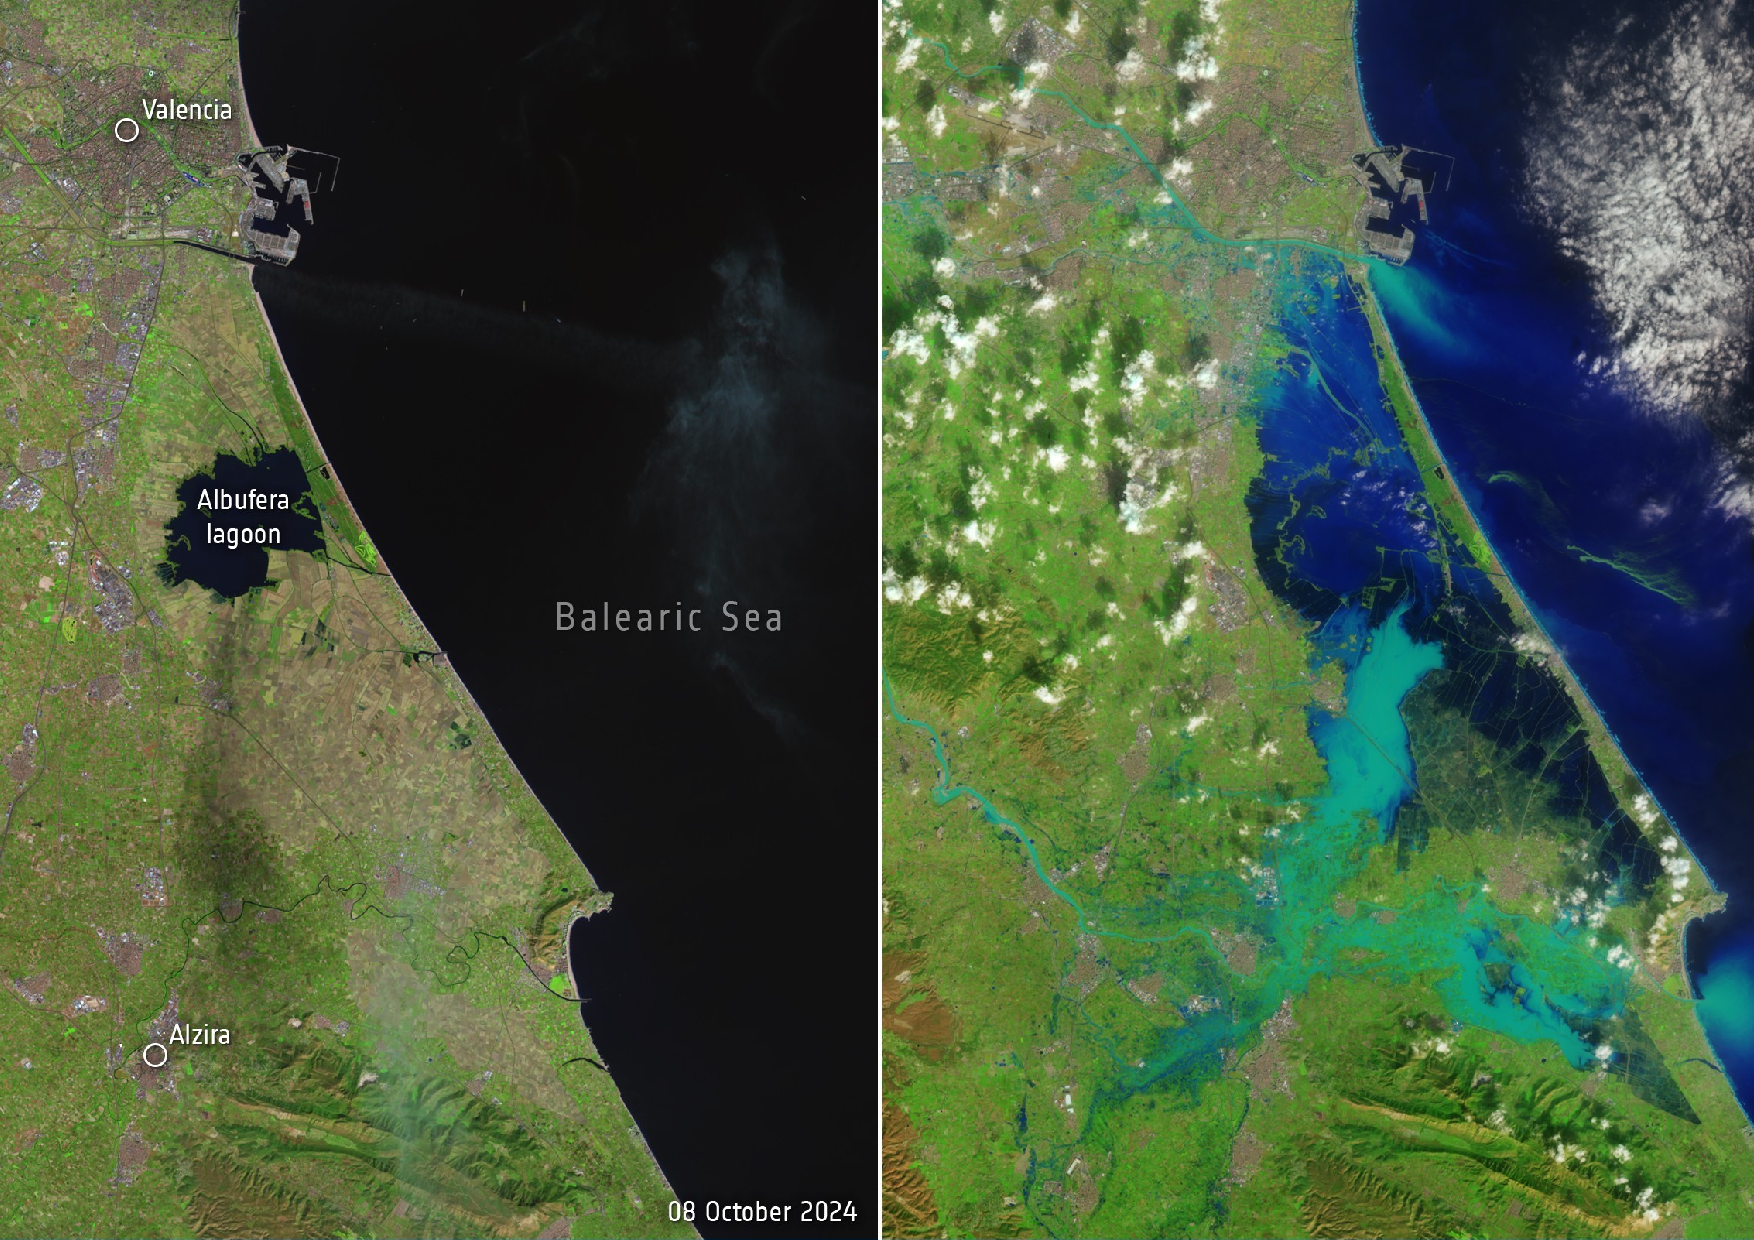
\includegraphics[width=0.7\textwidth]{C:/Users/Matteo/Shallow-Water-Equations/figs/photo_valencia.pdf}
    \caption{Before and after the floods in Valencia, Spain, October 2024.\\
            Source: \url{https://www.esa.int/ESA_Multimedia/Images/2024/10/Valencia_flood_disaster}.}
\end{figure}

\section{Motivation}
The Shallow Water Equations (SWE) are a set of hyperbolic partial differential equations that describe the motion of a fluid in a shallow layer of water.
These equations are crucial for understanding and simulating water dynamics in shallow water regions, such as coastal areas, rivers, and flood-prone regions.
A wide range of problems can be modeled by the shallow water equations, such as flooding, tsunamis and dam break scenarios.
Recent catastrophic events, such as the floods in the Valencia region of Spain in late October 2024, highlight the urgent need for efficient tools to simulate and understand flood behavior.
On October 29, 2024, Valencia received a years worth of rain in just eight hours, leading to flash floods that devastated the area, resulting in significant loss of life and property damage~\cite{valencia_flood_disaster_esa}.

While it is impossible to prevent such disasters from occurring, a robust toolkit to solve the shallow water equations can help us simulate the spreading of floods quickly.
This can aid in emergency response and disaster management.
The ability to rapidly simulate flood scenarios could significantly reduce the time needed for decision-making in critical situations.
Traditional numerical methods already exist to solve the SWE, but their accuracy often comes at the cost of high computational demands.
In many cases, the run time can be too long, meaning simulations may be too slow to provide real-time insight during a flood event.
This motivates the investigation of data-driven approaches to solve the SWE faster while maintaining an acceptable level of accuracy.

By investigating data-driven methods, this project aims to determine whether they can offer a faster and more efficient way to solve the shallow water equations compared to traditional numerical methods, ultimately improving our ability to respond to and manage flooding disasters.
In this work, we will derive the SWE in 1D, 2D, and spherical coordinates to model the flow of water on the Earth's surface.
We will explore the Finite Volume Method (FVM) in 1D and 2D, a numerical technique for solving partial differential equations by dividing the domain into small control volumes and integrating the equations over these volumes.
This method is widely used in computational fluid dynamics to model fluid behavior.
We will implement the FVM and use it to solve the SWE in 1D for several problems, including the dam break problem. We will then extend this approach to 2D and solve the idealized circular dam break problem.
The FVM solvers will be validated by comparing them with known test cases, as this validation is critical for generating the data needed to train the data-driven approaches, such as Convolutional Neural Networks (CNN) and Fourier Neural Operators (FNO).
The data-driven models will be trained and evaluated based on key performance metrics such as run time, accuracy, long-term prediction capabilities (i.e., their ability to generalize to unseen data), grid transferability, and their response to new initial conditions.
These initial conditions could include varying water heights, velocities, and other environmental factors that may change in real-world flood scenarios.
We will analyze the advantages and disadvantages of these data-driven methods and compare their run times with those of traditional numerical methods.
This comparison will allow us to assess whether data-driven approaches offer a practical solution to efficiently solving the shallow water equations, ultimately improving disaster response and flood prediction, even under varying and unforeseen initial conditions.

\section{Literature}
When working in this area it inevitably to mention the work of E. F. Toro, who has written several books on the topic of Riemann solvers and the Finite Volume Method, specifically for the shallow water equations.
In this project, we will use the books \textit{Shock-Capturing Methods for Free-Surface Shallow Flows}~\cite{Toro2001-Shock}, \textit{Riemann Solvers and Numerical Methods for Fluid Dynamics}~\cite{Toro2009-Riemann} and the rather new book from 2024 \textit{Computational Algorithms for Shallow Water Equations}~\cite{Toro2024} as references.
The books have been especially useful when deriving the shallow water equations and the Riemann solvers used in this project, as well as understanding and describing the Finite Volume Method.
The course \textit{Advanced Numerical Methods for Environmental Models} at the University of Trento, has provided a good foundation for the numerical methods used in this project, both in terms of lecture notes and exercises~\cite{trento_course}.

Working with the shallow water equations in spherical coordinates, the papers \textit{Well-balanced methods for the shallow water equations in spherical coordinates} by Castro et al.~\cite{Castro2017} and \textit{Physics-informed neural networks for the shallow-water equations on the sphere} by Bihlo et al.~\cite{Bihlo2022} are key references for deriving the SWE in spherical coordinates.
Additionally, the lecture notes \textit{Shallow water on a sphere} by Raymond from New Mexico Tech~\cite{Raymond} have been valuable in this derivation.
Further, the papers by Gavete~\cite{Gavete_2009} and Galewsky~\cite{Galewsky_2004} also provide important insights into the spherical shallow water equations.
Implementing the FVM to solve the shallow water equations in spherical coordinates is a challenging task, as exact literature on the topic is limited.
However, some sources discussing the Discontinuous Galerkin scheme for solving the spherical shallow water equations have been somewhat useful in this context.

The field of Fourier Neural Operators (FNO) is relatively new, and as a result, there is limited literature on the topic.
However, the paper \textit{Fourier Neural Operator for Parametric Partial Differential Equations}~\cite{FNO_2021}, written by several authors, is a key reference.
In the last years the company Nvidia has done some very interesting work on the topic of FNO, and they have published several blog posts on the topic.
One of the posts consider the use of Spherical Fourier Neural Operators (SFNO) to generate weather forecasts around the globe\cite{Nvidia2023}.
Another paper is~\cite{bonev2023-SFNO}.
These papers suggest that FNOs has shown great potential in being an efficient and resolution independent operator in the field of scientific machine learning.
Suggested, a key reason their success is their ability to make long-term predictions. 
The papers also explains the introduction of Spherical FNOs (SFNOs) for learning operators on spherical geometries.
Convolutional Neural Networks (CNNs) are a well-researched area, with numerous sources available on the topic.
For this project, the sources~\cite{oshea2015introductionconvolutionalneuralnetworks} and~\cite{chollet2017comprehensive} have been particularly helpful in explaining the theoretical foundations of the methods.

\section{Thesis overview}
In \autoref{ch:theory}, we derive the shallow water equations in 1D, 2D, and spherical coordinates.
In \autoref{ch:fvm}, we present the Finite Volume Method (FVM) used to solve the shallow water equations, including the Riemann problem and the numerical fluxes essential for the FVM.
These chapters form the theoretical and methodological foundation for the numerical methods employed in this project, leading into the discussion of data-driven methods.

In \autoref{ch:FNO+NN}, we introduce the concepts of Fourier Neural Operators (FNO) and Convolutional Neural Networks (CNN), explaining how these methods can be applied to solve the shallow water equations.
In \autoref{ch:method}, we describe the process of generating the data required for the data-driven methods, as we produce all the data used in this project ourselves.

Chapter~\ref{ch:numerical_results} focuses on the numerical results for the 1D and 2D shallow water equations using the FVM.
To validate these results, we compare the FVM outputs with test cases from the literature. Validation is crucial since the data-driven models are trained on the FVM data.
In \autoref{ch:data-driven-results}, we present the results for the shallow water equations using the data-driven models, comparing performance in terms of runtime and accuracy.
We analyze the outcomes, discuss the performance of the data-driven models, and compare them to the numerical results.

Finally, in \autoref{ch:discussion}, we discuss the findings, and in \autoref{ch:conclusion}, we conclude the thesis and propose directions for future work.




\newpage
\chapter{The Shallow Water Equations}\label{ch:theory}
In this chapter, we explore the theory behind the shallow water equations (SWE).
We begin by introducing the relevant notation used throughout the report.
Next, we derive the SWE in conservative form and present them in both vector and integral form for both the 1D- and 2D-case in cartesian coordinates.
We extend the derivation to spherical coordinates, where we derive the nonlinear SWE and afterwards linearize the equations.

\section{Notation}
Before deriving the shallow water equations (SWE), we will introduce the notation that will be used throughout this report.
In both the 1D and 2D cases of SWE, we use cartesian coordinates $(x, y, z)$ with time denoted by $t$.
Given that linear algebra is a fundamental tool used in this report, we first establish the relevant notation.
Lowercase bold letters represent vectors, while uppercase bold letters represent matrices.
For instance, $\mathbf{a}$ is a vector of size $1 \times r, r \in \mathbb{R}$, and $\mathbf{A}$ is a matrix of size $m \times n, m,n \in \mathbb{R}$.
The identity matrix, denoted by $\mathbf{I}$, is a square matrix with ones along the diagonal and zeros elsewhere.
For example, the $3 \times 3$ identity matrix is given by:
\begin{align*}
    \mathbf{I} = \begin{bmatrix}
        1 & 0 & 0 \\
        0 & 1 & 0 \\
        0 & 0 & 1
    \end{bmatrix}.
\end{align*}
We use the following notation for partial derivatives:
\begin{align*}
   f_x =  \frac{\partial f}{\partial x}, \quad f_y = \frac{\partial f}{\partial y}, \quad f_z = \frac{\partial f}{\partial z}.
\end{align*}
The gradient operator, denoted by $\nabla$, gives the gradient of a scalar function $f$ as a vector:
\begin{align*}
    \nabla f = \begin{bmatrix}
        \frac{\partial f}{\partial x} &
        \frac{\partial f}{\partial y} &
        \frac{\partial f}{\partial z}
    \end{bmatrix}.
\end{align*}
Given two vectors $\mathbf{a} = \begin{bmatrix}
    a_1 & a_2 & a_3
\end{bmatrix}^\top $ and $\mathbf{b} = \begin{bmatrix}
    b_1 & b_2 & b_3
\end{bmatrix}^\top$, the dot product of $\mathbf{a}$ and $\mathbf{b}$ is given by:
\begin{align*}
    \mathbf{a} \cdot \mathbf{b} = a_1 b_1 + a_2 b_2 + a_3 b_3.
\end{align*}
The dot product can also be written as a matrix product:
\begin{align*}
    \mathbf{a} \cdot \mathbf{b} = \mathbf{a}^\top \mathbf{b}.
\end{align*}
The divergence operator, represented as $\nabla \cdot $, gives the divergence of a vector $\mathbf{a}$ as:
\begin{align*}
    \nabla \cdot \mathbf{a} = \frac{\partial a_1}{\partial x} + \frac{\partial a_2}{\partial y} + \frac{\partial a_3}{\partial z} = {a_1}_x + {a_2}_y + {a_3}_z.
\end{align*}
The tensor product of two vectors $\mathbf{a}$ and $\mathbf{b}$, denoted as $\mathbf{a} \otimes \mathbf{b}$, is a matrix where each element is the product of the elements of $\mathbf{a}$ and $\mathbf{b}$, i.e.,
\begin{align*}
    \mathbf{a} \otimes \mathbf{b} = \begin{bmatrix}
        a_1 b_1 & a_1 b_2 & a_1 b_3 \\
        a_2 b_1 & a_2 b_2 & a_2 b_3 \\
        a_3 b_1 & a_3 b_2 & a_3 b_3
\end{bmatrix}.
\end{align*}






\section{Derivation of the SWE with conservative variables}
The shallow water equations are derived from the conservation laws for mass and momentum, and are fundamental in fluid dynamics.
The derivation follows four steps: First we consider the conservation laws for mass and momentum, and then we consider the boundary conditions for a free surface problem.
Afterwards we make some neccessary assumptions and finally we use the boundary conditions to integrate the conservation laws over depth.
The derivation follows the methods outlined in~\cite{Toro2001-Shock} and~\cite{Vreugdenhil1994}.


\subsubsection*{Conservation laws}
The conservation laws for mass and momentum state that the total mass and momentum are conserved over time.
The conservation laws for mass and momentum can be expressed generally as follows~\cite[eq.'s (2.1) and (2.2)]{Toro2001-Shock}:
\begin{subequations}
    \begin{align}
        \rho_t + \nabla \cdot (\rho \mathbf{v}) = 0, \label{eq:mass_conservation} \\
        {(\rho \mathbf{v})}_t + \nabla \cdot (\rho \mathbf{v} \otimes \mathbf{v} + p \mathbf{I} - \mathbf{T}) = \rho \mathbf{g}, \label{eq:momentum_conservation}
    \end{align}
  \end{subequations}
where $\rho$ is the fluid density, $\mathbf{v} = \begin{bmatrix} u & v & w \end{bmatrix}^\top$ is the fluid velocity in the $x, y$ and $z-$direction respectively,
$p$ is the pressure, $\mathbf{I}$ is the identity matrix, and the vector $\mathbf{g} = \begin{bmatrix}
    g_1 & g_2 & g_3
\end{bmatrix}^\top$ represents body forces including gravity.
In these equations, the density $\rho$ and the pressure $p$ are dependent of $x, y, z$ and $t$, but later we will introduce some assumptions that simplify the equations.
The matrix $\mathbf{T}$ is the viscous stress tensor, given by
\begin{align*}
    \mathbf{T} = \begin{bmatrix}
        \tau_{xx} & \tau_{xy} & \tau_{xz} \\
        \tau_{yx} & \tau_{yy} & \tau_{yz} \\
        \tau_{zx} & \tau_{zy} & \tau_{zz}
    \end{bmatrix},
\end{align*}
which accounts for the viscous forces in the fluid.
However, in this project the viscous stress tensor $\mathbf{T}$ is neglected, since we assume the function $\tau(x,y,z)$ is constant.
The matrix $\mathbf{v} \otimes \mathbf{v}$ represents the tensor product of the velocity vector $\mathbf{v}$ with itself, i.e.,
\begin{align*}
    \mathbf{v} \otimes \mathbf{v} = \begin{bmatrix}
        u^2 & uv & uw \\
        vu & v^2 & vw \\
        wu & wv & w^2
    \end{bmatrix}.
\end{align*}
Note that $\mathbf{v} \otimes \mathbf{v} = \mathbf{v} \mathbf{v}^\top$.
Putting this together, we can rewrite the momentum equation~\eqref{eq:momentum_conservation} as
\begin{align}\label{eq:momentum_conservation_simplified}
    {(\rho \mathbf{v})}_t + \nabla \cdot (\rho \mathbf{v} \mathbf{v}^\top  + p \mathbf{I}) - \rho \mathbf{g} = 0.
\end{align}
Applying the divergence operator and the product rule for differentiation, we can write out the mass equation~\eqref{eq:mass_conservation} as
\begin{align}\label{eq:mass_cons_derive}
    \rho_t + \rho(u_x + v_y + w_z) + u \rho_x + v \rho_y + w \rho_z = 0.
\end{align}
In this project we consider incompressible fluids, meaning that the fluid density $\rho$ is independent of the pressure $p$.
We also assume that the fluid density only depends on temperature and salinity, and thus is independent of $t, x, y$ and $z$.
Additionally, we assume $\rho$ is nonzero.
Hence from~\eqref{eq:mass_cons_derive} we obtain
\begin{align}
    u_x + v_y + w_z = 0, \label{eq:mass_conservation_incompressible}
\end{align}
also referred to as the mass conservation equation.
Applying the divergence operator $\nabla \cdot$, the momentum conservation equation~\eqref{eq:momentum_conservation_simplified} can be written out as:
\begin{align}\label{eq:momentum_conservation_expanded}
    \rho_t \mathbf{v} + \rho \mathbf{v}_t + \rho \begin{bmatrix}
        {(u^2 + p)}_x + {(uv)}_y + {(uw)}_z \\
        {(vu)}_x + {(v^2 + p)}_y + {(vw)}_z \\
        {(wu)}_x + {(wv)}_y + {(w^2 + p)}_z 
    \end{bmatrix}
    - \rho \mathbf{g} = 0.
\end{align}
We neglect all body forces in $\mathbf{g}$, expect the gravitational force in the $z-$direction, i.e., $\mathbf{g} = \begin{bmatrix} 0 & 0 & -g \end{bmatrix}$, where $g$ is the gravity acceleration, which we assume to be constant.
Hence, by using the product rule in~\eqref{eq:momentum_conservation_expanded} and that $\rho_t = 0$ we obtain
\begin{align}\label{eq:momentum_conservation_expanded_final}
    \rho \begin{bmatrix}
        u_t \\ v_t \\ w_t
    \end{bmatrix}
    + \rho \begin{bmatrix}
        p_x + u u_x + v u_y + w u_z + u(u_x + v_y + w_z) \\
        p_y + u v_x + v v_y + w v_z + v(u_x + v_y + w_z) \\
        p_z + u w_x + v w_y + w w_z + w(u_x + v_y + w_z) 
    \end{bmatrix}
    - \rho \begin{bmatrix}
        0 \\ 0 \\ -g
    \end{bmatrix} = 0.
\end{align}
We apply~\eqref{eq:mass_conservation_incompressible} to~\eqref{eq:momentum_conservation_expanded_final} to remove terms, we move the pressure terms to the right hand side, and we divide by $\rho$.
Putting it all together, the mass equation~\eqref{eq:mass_conservation} and the momentum equation~\eqref{eq:momentum_conservation_simplified}, split in $x, y$ and $z-$directions, simplify to 
\begin{equation}\label{eq:momentum_conservation_all}
    \left.
    \begin{aligned}
        u_x + v_y + w_z &= 0, \\
        u_t + u u_x + v u_y + w u_z &= - \frac{1}{\rho} p_x, \\
        v_t + u v_x + v v_y + w v_z &= - \frac{1}{\rho} p_y, \\
        w_t + u w_x + v w_y + w w_z &= - \frac{1}{\rho} p_z - g.
    \end{aligned}
    \right\}
\end{equation}


\subsubsection*{Boundary conditions}
The focus is on the flow of water with a free surface, meaning that the surface is not fixed and can move or change over time.
To solve the SWE, it is essential to impose boundary conditions at both the bottom of the water column and at the free surface.
We assumme the bottom $b$ is defined by a function
\begin{align*}
    z = b(x,y),
\end{align*}
meaning that the bottom is dependent on $x$ and $y$, but not on the time $t$.
Since the bottom is not moving over time, we refer to it as fixed.
The free surface is defined by 
\begin{align*}
    z = s(x,y,t) \equiv b(x,y) + h(x,y,t),
\end{align*}
where $h(x,y,t)$ is the water depth at time $t$.
The following illustration helps to visualize the setup:
\begin{figure}[H]
    \centering
    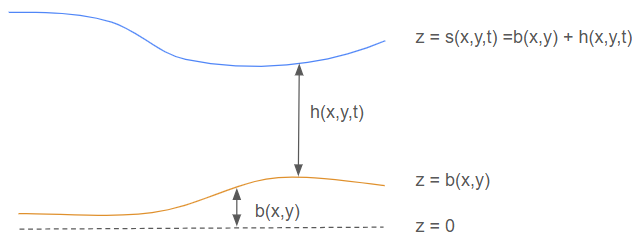
\includegraphics[width=0.6\textwidth]{figs/water-column-bc.png}
    \caption{Illustration of a water column with a free surface.}\label{fig:water_column_bc}
\end{figure}
We impose boundary conditions at the bottom and at the free surface, adressing both kinematic and dynamical conditions.
To describe the boundaries mathematically, we introduce a boundary function $\psi(x,y,z,t)$ that is zero on the boundaries:
\begin{align*}
    \psi(x,y,z,t) = 0.
\end{align*}
For the free surface, this boundary is given by
\begin{align}\label{eq:psi_free_surface}
    \psi|_{z = s} = z - s(x,y,t) = 0,
\end{align}
and for the bottom, it is described by
\begin{align}\label{eq:psi_bottom}
    \psi|_{z = b} = z - b(x,y) = 0.
\end{align}
In deriving a kinematic condition, we assume that fluid particles on the boundary remain on the boundary over time.
Mathematically this is expressed as
\begin{align*}
    \frac{\text{d} }{\text{d} t} \psi(x,y,z,t) = 0.
\end{align*}
Recall, that $\frac{\partial \psi}{\partial t}$ is the partial derivative of $\psi$ with respect to $t$, while the total derivate $\frac{\text{d} \psi}{\text{d} t}$ accounts for both the direct change of $\psi$ with respect to $t$ and the changes due to the movement of the fluid in the $x, y$ and $z$ directions.
Hence, the total derivative of $\psi$ wrt. $t$ is given by
\begin{align*}
    \frac{\text{d} \psi}{\text{d} t} &= \frac{\partial \psi}{\partial t} + \frac{\text{d} x}{\text{d} t} \frac{\partial \psi}{\partial x} + \frac{\text{d} y}{\text{d} t}  \frac{\partial \psi}{\partial y} + \frac{\text{d} z}{\text{d} t}  \frac{\partial \psi}{\partial z}.
\end{align*}
We see that $\frac{\text{d}x}{\text{d}t}$ denotes the velocity in the $x-$direction, i.e., $u$, and correspondingly $\frac{\text{d}y}{\text{d}t}$ and $\frac{\text{d}x}{\text{d}t}$ denotes $v$ and $w$ respectively.
Thus, the kinematic condition is given by
\begin{align}\label{eq:kinematic_condition}
    \frac{\text{d} }{\text{d} t} \psi = \psi_t + u \psi_x + v \psi_y + w \psi_z = 0.
\end{align}
Applying this to the free surface by substituting~\eqref{eq:psi_free_surface} into the kinematic condition~\eqref{eq:kinematic_condition} yields
\begin{align}\label{eq:kinematic_condition_free_surface}
    (s_t + u s_x + v s_y - w)|_{z=s} = 0.
\end{align}
Similarly, for the bottom, substitung~\eqref{eq:psi_bottom} into the kinematic condition~\eqref{eq:kinematic_condition} gives
\begin{align}\label{eq:kinematic_condition_bottom}
    (u b_x + v b_y - w)|_{z=b} = 0.
\end{align}
The dynamical condition is related to the pressure distribution at the free surface.
We assume that the pressure at the free surface is equal to the pressure in the air above the surface, that is, the atmospheric pressure.
Since absolute pressure levels are irrelevant, as we are primarily concerned with pressure differences, we set the pressure at the free surface to zero.
This leads to the following expression for the pressure at the free surface:
\begin{align}\label{eq:pressure_free_surface}
    p(x,y,z,t)|_{z = s} = 0.
\end{align}
This condition, known as the dynamical condition, relates to the forces acting on the boundaries of the fluid.

\subsubsection*{Assumptions}
To derive the SWE it is neccessary to make some physical assumptions. 
The shallow water equations are an approximation to the full free-surface problem and result from the assumption that the vertical compononent of the acceleration is negligible.
Therefore, we begin by assuming that the vertical acceleration, represented by the total derivative of the vertical velocity component $w$ with respect to time, is negligible.
This assumption leads to the condition
\begin{align*}
    \frac{\text{d} w}{\text{d} t} = w_t + uw_x + vw_y + ww_z = 0.
\end{align*}
Applying $\frac{\text{d}w}{\text{d}t} = 0$ in the $z-$momentum conservation equation~\eqref{eq:momentum_conservation_all} simplifies it to
\begin{align*}
    p_z = -\rho g.
\end{align*}
By using properties of an integral, together with~\eqref{eq:pressure_free_surface} we get
\begin{align*}
    \int_{b(x,y)}^z - \rho g \text{ d}t + \int_z^{s(x,y,t)} - \rho g \text{ d}t = \int_{b(x,y)}^{s(x,y,t)} - \rho g \text{ d}t
    = p|_{z = s(x,y,t)} = 0.
\end{align*}
This implies that the pressure distribution follows
\begin{align}\label{eq:pressure_distribution}
    p = \int_{b(x,y)}^z - \rho g \text{ d}t = \int_z^{s(x,y,t)} \rho g \text{ d}t = \rho g (s - z),
\end{align}
where $s$ is the surface height.
Differentiating~\eqref{eq:pressure_distribution} with respect to $x$ and $y$ yields
\begin{align*}%\label{eq:pressure_distribution_x_y}
    p_x = \rho g s_x, \quad p_y = \rho g s_y.
\end{align*}
Substituting these expressions into the $x-$ and $y-$momentum conservation equations~\eqref{eq:momentum_conservation_all} leads to 
\begin{equation}\label{eq:momentum_conservation_xy_simplified}
    \left.
    \begin{aligned}
        u_t + u u_x + v u_y + w u_z &= -g s_x,  \\
        v_t + u v_x + v v_y + w v_z &= -g s_y,
    \end{aligned}
    \right\}
\end{equation}
which can be further simplified.
We realize that both $p_x$ and $p_y$ are independent of $z$, implying that $\frac{\text{d}u}{\text{d}t} $ and $\frac{\text{d}v}{\text{d}t} $are also independent of $z$.
Hence $u_z = v_z = 0$, implying that~\eqref{eq:momentum_conservation_xy_simplified} can be simplified to
\begin{equation}\label{eq:momentum_conservation_xy_final}
    \left.
    \begin{aligned}
        u_t + u u_x + v u_y &= -g s_x,  \\
        v_t + u v_x + v v_y &= -g s_y.
    \end{aligned}
    \right\}
\end{equation}
These are the momentum equations for the shallow water equations in two spatial dimensions.

\subsubsection*{Integration over depth}
The next step in deriving the SWE is to integrate the conservation equations over the vertical direction $z$.
We integrate the mass conservation equation~\eqref{eq:mass_conservation_incompressible} and the momentum conservation equations in~\eqref{eq:momentum_conservation_xy_final}, from the bottom, $z = b(x,y)$ to the free surface, $z = s(x,y,t)$.
Starting with the mass conservation equation~\eqref{eq:mass_conservation_incompressible}, we have
\begin{align*}
    \int_{b}^{s} u_x + v_y + w_z \text{ d} z = 0,
\end{align*}
implying that, using linearity of the integral, we get
\begin{align}\label{eq:mass_conservation_integrated}
    \int_{b}^{s} u_x \text{ d} z + \int_{b}^{s} v_y \text{ d} z  + w|_{z = s} - w|_{z = b} = 0.
\end{align}
We will use Leibniz's integral rule~\cite{Leibniz}, which is stated as follows:
\begin{align}\label{eq:leibniz_rule}
    \frac{\text{d}}{\text{d} x} \int_{a(x)}^{b(x)} f(x,t) \text{ d} t
    = \int_{a(x)}^{b(x)} \frac{\partial }{\partial x} f(x, t) \text{ d} t + f(x, b(x)) \frac{\text{d}}{\text{d} x} b(x) - f(x, a(x)) \frac{\text{d}}{\text{d} x} a(x),
\end{align}
to integrate the first two terms in~\eqref{eq:mass_conservation_integrated}, which yields
\begin{align}\label{eq:leibniz_rule_applied}
    \begin{gathered}
        \left.
        \begin{aligned}
        \int_{b}^{s} u_x \, \text{d} z &=  \frac{\text{d}}{\text{d} x}  \int_{b}^{s} u \, \text{d} z  - u|_{z = s} \frac{\text{d} s}{\text{d} x} + u|_{z = b} \frac{\text{d} b}{\text{d} x}, \\
        \int_{b}^{s} v_y \, \text{d} z &=  \frac{\text{d}}{\text{d} y}  \int_{b}^{s} v \, \text{d} z  - v|_{z = s} \frac{\text{d} s}{\text{d} y} + v|_{z = b} \frac{\text{d} b}{\text{d} y}.
        \end{aligned}
        \right\}
    \end{gathered}
\end{align}
Note that since a change in $x$ does not affect the $y$-component of the bottom or surface, we have that $\frac{\text{d} s}{\text{d} x} = s_x$ and $ \frac{\text{d} b}{\text{d} x} = b_x$, and correspondingly for $s_y$ and $b_y$.
Likewise we can substitute $\frac{\text{d}}{\text{dx}}$ with $\frac{\partial}{\partial x}$ in the integrals, since the integrals are with respect to $z$, and $u$ and $v$ are independent of $z$.
Inserting these results in~\eqref{eq:leibniz_rule_applied} gives
\begin{align}\label{eq:leibniz_rule_applied_final}
    \begin{gathered}
        \left.
            \begin{aligned}
                \int_{b}^{s} u_x \text{ d} z &=  \frac{\partial}{\partial x}  \int_{b}^{s} u \text{ d} z  - u|_{z = s} s_x + u|_{z = b} b_x, \\
                \int_{b}^{s} v_y \text{ d} z &= \frac{\partial}{\partial y}  \int_{b}^{s} v \text{ d} z  - v|_{z = s} s_y + v|_{z = b} b_y.
            \end{aligned}
        \right\}
    \end{gathered}
\end{align}
We can now insert the integrals~\eqref{eq:leibniz_rule_applied_final} into the integrated mass conservation equation~\eqref{eq:mass_conservation_integrated} to get
\begin{align}\label{eq:mass_conservation_integrated_final}
    \frac{\partial}{\partial x}  \int_{b}^{s} u \text{ d} z  - u|_{z = s} s_x + u|_{z = b} b_x
    + \frac{\partial}{\partial y}  \int_{b}^{s} v \text{ d} z  - v|_{z = s} s_y + v|_{z = b} b_y
    + w|_{z = s} - w|_{z = b} = 0.
\end{align}
To simplify this equation further, we consider the boundary conditions.
From~\eqref{eq:kinematic_condition_bottom} we have
\begin{align}
    w|_{z = b} = (u b_x + v b_y)|_{z = b},
\end{align}
and from~\eqref{eq:kinematic_condition_free_surface} we have
\begin{align}
    w|_{z = s} = (s_t + u s_x + v s_y)|_{z = s}.
\end{align}
We note that $s = b + h$ and hence $s_t = h_t$, as the bottom is fixed.
Recall that $u$ and $v$ are independent of $z$, and the water depth is $h = s - b$, meaning we have
\begin{align*}
    \int_{b}^{s} u \text{ d} z = u(s - b) = hu, \quad \int_{b}^{s} v \text{ d} z = v(s - b) = hv.
\end{align*}
Putting it all together the equation~\eqref{eq:mass_conservation_integrated_final} simplifies to
\begin{align}\label{eq:SWE_1}
    h_t + {(hu)}_x + {(hv)}_y = 0,
\end{align}
which is also the first equation in the SWE stated in conservative form.
When integrating the momentum equations~\eqref{eq:momentum_conservation_xy_final} over the vertical direction, we see that since the equations are independent of $z$, the resulting equations are simply
\begin{equation}\label{eq:xy_momentum}
    \left.
    \begin{aligned}
        h(u_t + uu_x + vu_y + g s_x) &= 0,\\
        h(v_t + uv_x + vv_y + g s_y) &= 0.
    \end{aligned}
    \right\}
\end{equation}
We multiply~\eqref{eq:SWE_1} with $u$ and $v$ respectively, and add the resulting two equations to~\eqref{eq:xy_momentum}.
Recall that $s = h + b$. 
By using the product rule for differentiation and collecting terms, we obtain the momentum equations stated in conservative form:
\begin{equation}\label{eq:SWE_2}
    \left.
    \begin{aligned}
        {(hu)}_t + {(hu^2 + \frac{1}{2}gh^2)}_x + {(huv)}_y &= -gh b_x,\\
        {(hv)}_t + {(huv)}_x + {(hv^2 + \frac{1}{2}gh^2)}_y &= -gh b_y.
    \end{aligned}
    \right\}
\end{equation}
The three partial differential equations in~\eqref{eq:SWE_1} and~\eqref{eq:SWE_2} are the shallow water equations stated in conservative form.

\section{The SWE in vector form}
We present the SWE in vector form, which is useful as it allows all three partial differential equations to be combined into a single unified equation.
The SWE can be written in differential conservation law form as the vector equation
\begin{align}\label{eq:vector_form_2D}
    \mathbf{U}_t + \mathbf{F(U)}_x + \mathbf{G(U)}_y = \mathbf{S(U)},
\end{align}
where 
\begin{align*}
    \mathbf{U} = \begin{bmatrix}
        h \\
        hu \\
        hv
    \end{bmatrix},
    \quad 
    \mathbf{F(U)} = \begin{bmatrix}
        hu \\
        hu^2 + \frac{1}{2}gh^2 \\
        huv
    \end{bmatrix},
    \quad
    \mathbf{G(U)} = \begin{bmatrix}
        hv \\
        huv \\
        hv^2 + \frac{1}{2}gh^2
    \end{bmatrix}
    \quad \text{and} \quad
    \mathbf{S(U)} = \begin{bmatrix}
        s_1 \\
        s_2 \\
        s_3
    \end{bmatrix} = 
    \begin{bmatrix}
        0 \\
        -gh b_x \\
        -gh b_y
    \end{bmatrix}
    .
\end{align*}
We call $\mathbf{U}$ the vector of conserved variables, $\mathbf{F(U)}$ and $\mathbf{G(U)}$ the flux vectors in the $x-$ and $y-$direction, and $\mathbf{S(U)}$ the source term vector.
Note that the source term vector $\mathbf{S(U)}$ often includes additional terms, such as friction and other external forces.
However, since only gravity is considered in this case, the source term vector is simplified to the expression shown above.
Moreover, if $\mathbf{S(U)} = 0$, then we consider a homogeneous equation, and if $\mathbf{S(U)} \neq 0$, we consider an inhomogeneous equation.

We also consider the one-dimensional case of the SWE in vector form, where the flow is only in the $x-$direction.
The vector form of the SWE in 1D is given by
\begin{align}\label{eq:vector_form_1D}
    \mathbf{U}_t + \mathbf{F(U)}_x = \mathbf{S(U)},
\end{align}
where
\begin{align}\label{eq:vector_form_1D_variables}
    \mathbf{U} = \begin{bmatrix}
        h \\
        hu
    \end{bmatrix},
    \quad
    \mathbf{F(U)} = \begin{bmatrix}
        hu \\
        hu^2 + \frac{1}{2}gh^2
    \end{bmatrix}
    \quad
    \text{and} \quad
    \mathbf{S(U)} = \begin{bmatrix}
        0 \\
        -gh b_x
    \end{bmatrix}.
\end{align}
When deriving numerical schemes in the finite volume method (FVM), the vector form of the 1D SWE can be used as a foundation.
The 1D formulation is preferred over the 2D version for this purpose because the principles underlying the numerical schemes remain the same in both dimensions.
Using the 1D SWE provides a simpler framework to introduce and analyze core aspects of the method, such as flux evaluation, conservation laws, and the treatment of source terms.
Once these concepts are well-understood in 1D, the method can be extended to 2D by applying similar principles, with modifications to account for the additional spatial dimension and the directional components of fluxes and source terms.

\section{The 1D SWE in integral form}
It is often more convenient to work with the integral form of the SWE, since the integral form of equations of the form~\eqref{eq:vector_form_2D} and~\eqref{eq:vector_form_1D} allows discountinuous solutions.
We derive the integral form of the inhomogenous one-dimensional case of the SWE in vector form~\eqref{eq:vector_form_1D}.
The integral form is obtained by integrating the vector form~\eqref{eq:vector_form_1D} over a control volume $V$ in the $x,t$ plane
\begin{align*}
    V = [x_L, x_R] \times [t_1, t_2].
\end{align*}
The control volume is illustrated in Figure~\ref{fig:control_volume_1D}.
\begin{figure}[H]
    \centering
    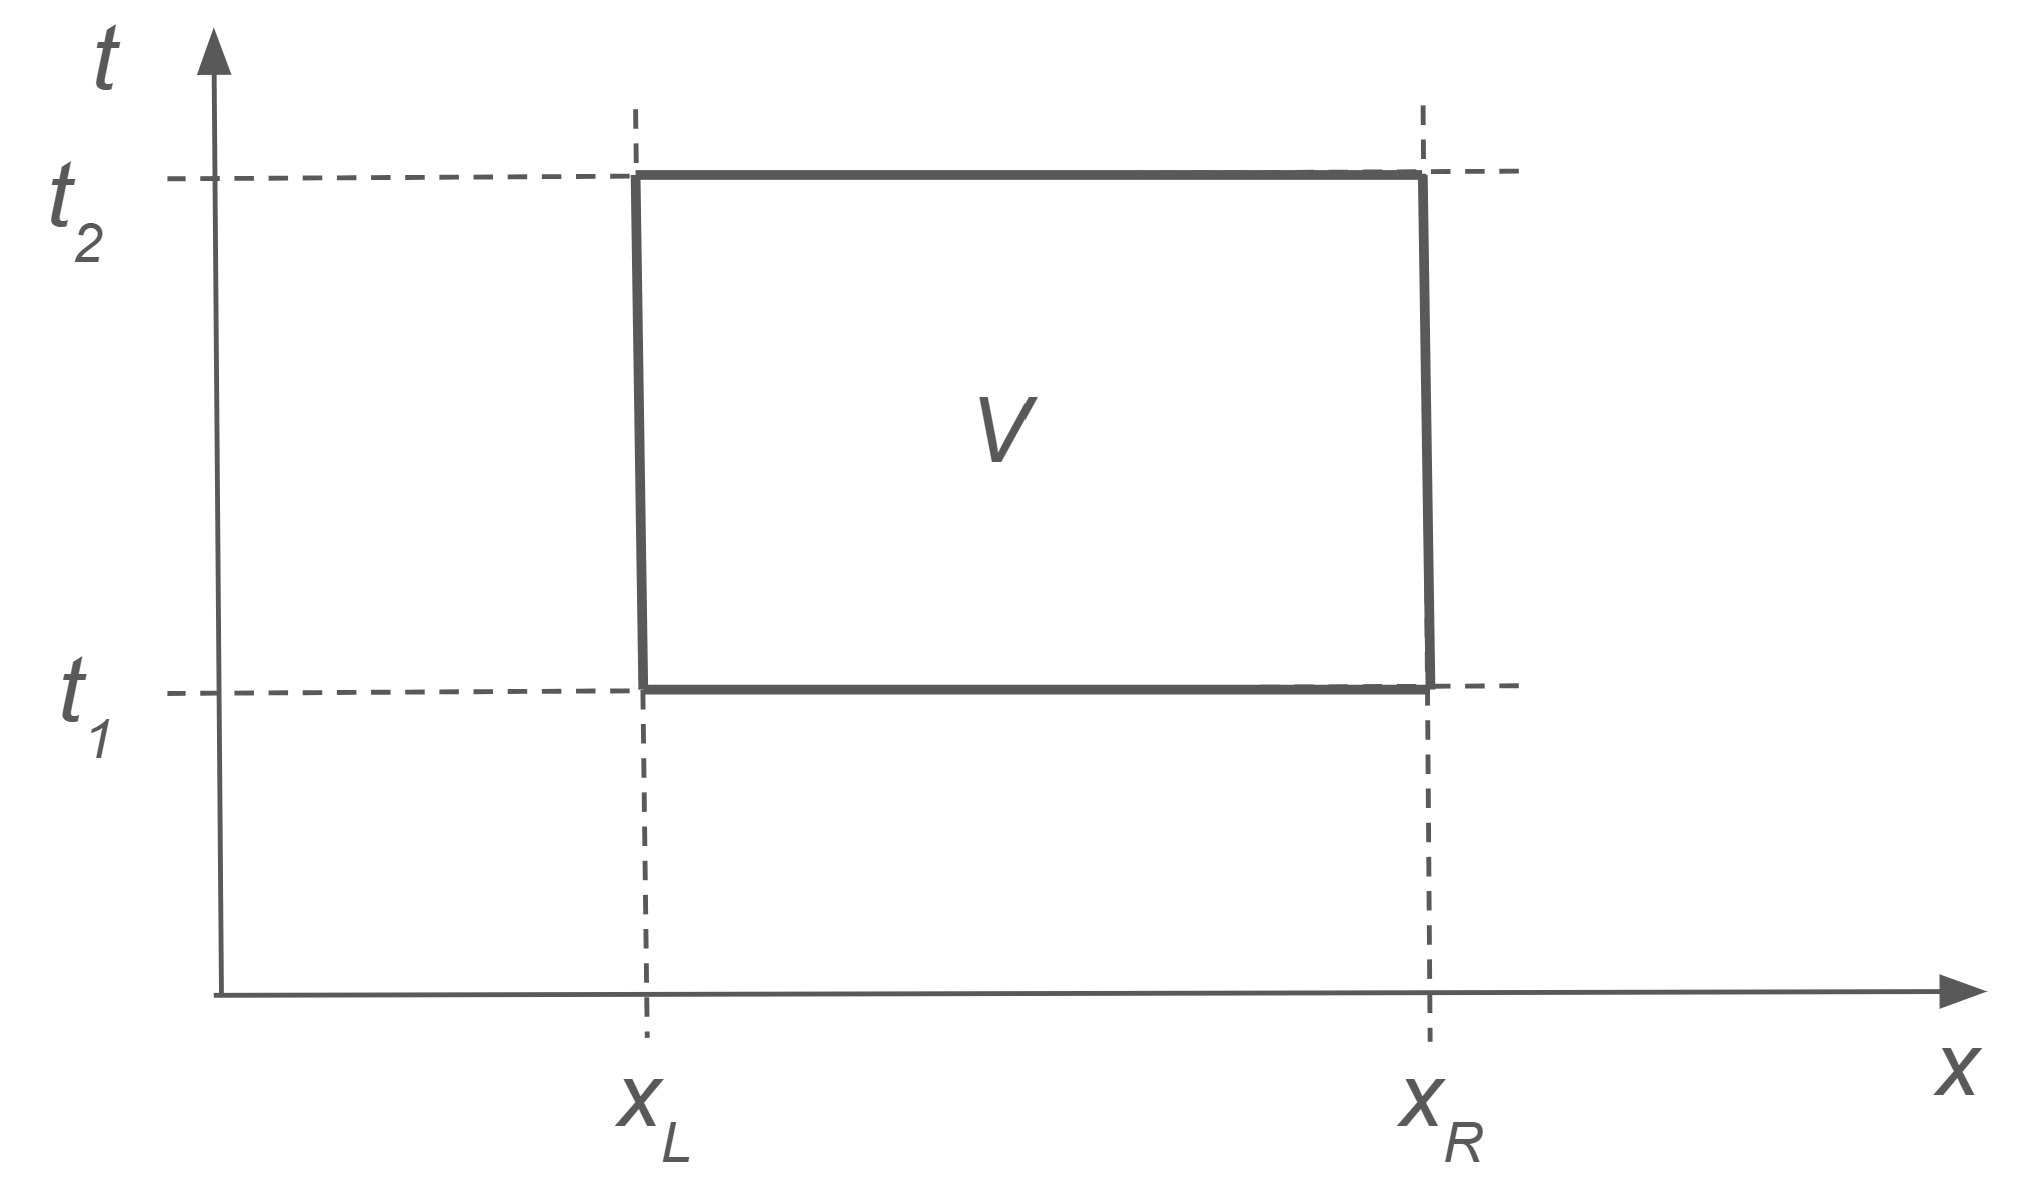
\includegraphics[width=0.5\textwidth]{C:/Users/Matteo/Shallow-Water-Equations/figs/Control_volume_1D.png}
    \caption{Illustration of a control volume $V$ in the $x,t$ plane. Illustration modified from~\cite{Toro2024}.}\label{fig:control_volume_1D}
\end{figure}
First we integrate the vector form of the SWE~\eqref{eq:vector_form_1D} over $x$ from $x_L$ to $x_R$ to obtain
\begin{align}\label{eq:derive_integral_form_1D}
    \int_{x_L}^{x_R} \mathbf{U}_t \text{ d}x + \int_{x_L}^{x_R} \mathbf{F(U)}_x \text{ d}x = \int_{x_L}^{x_R} \mathbf{S(U)} \text{ d}x.
\end{align}
Using the fundamental theorem of calculus, we get that 
\begin{align*}
    \int_{x_L}^{x_R} \mathbf{F}(\mathbf{U}) \text{ d}x = \mathbf{F}(\mathbf{U}(x_R, t)) - \mathbf{F}(\mathbf{U}(x_L, t)),
\end{align*}
which we insert in~\eqref{eq:derive_integral_form_1D}:
\begin{align}\label{eq:derive_integral_form_1D_2}
    \int_{x_L}^{x_R} \mathbf{U}_t \text{ d}x = \mathbf{F}(\mathbf{U}(x_L, t)) - \mathbf{F}(\mathbf{U}(x_R, t)) + \int_{x_L}^{x_R} \mathbf{S(U)} \text{ d}x.
\end{align}
Then we integrate~\eqref{eq:derive_integral_form_1D_2} over time from $t_1$ to $t_2$ to get
\begin{align*}
    \int_{t_1}^{t_2} \int_{x_L}^{x_R} \mathbf{U}_t \text{ d}x \text{d}t = \int_{t_1}^{t_2} \mathbf{F}(\mathbf{U}(x_L, t)) \text{ d}t - \int_{t_1}^{t_2} \mathbf{F}(\mathbf{U}(x_R, t)) \text{ d}t + \int_{t_1}^{t_2} \int_{x_L}^{x_R} \mathbf{S(U)} \text{ d}x \text{d}t.
\end{align*}
Rewriting the left hand side using the fundamental theorem of calculus, we get
\begin{align}\label{eq:integral_form_1D_final}
    \int_{x_L}^{x_R} \mathbf{U}(x, t_2) \text{ d}x =
    \int_{x_L}^{x_R}  \mathbf{U}(x, t_1) \text{ d}x + \int_{t_1}^{t_2} \mathbf{F}(\mathbf{U}(x_L, t)) \text{ d}t - \int_{t_1}^{t_2} \mathbf{F}(\mathbf{U}(x_R, t)) \text{ d}t + \int_{t_1}^{t_2} \int_{x_1}^{x_2} \mathbf{S(U)} \text{ d}x \text{d}t,
\end{align}
which is the integral form of the conservation laws for the SWE in 1D.
An alternative integral form of~\eqref{eq:vector_form_1D} is stated in~\cite{Toro2024}:
\begin{align}\label{eq:integral_form_1D_alternative}
    \frac{\text{d}}{\text{d}t} \int_{x_L}^{x_R} \mathbf{U}(x,t) \text{ d}x = \mathbf{F}(\mathbf{U}(x_L, t)) - \mathbf{F}(\mathbf{U}(x_R, t)) + \int_{x_L}^{x_R} \mathbf{S}(\mathbf{U}) \text{ d}x.
\end{align}
From~\eqref{eq:integral_form_1D_alternative} we get that the integral form of the homogeneous SWE in 1D is given by
\begin{align}\label{eq:integral_form_1D_homogeneous}
    \frac{\text{d}}{\text{d}t} \int_{x_L}^{x_R} \mathbf{U}(x,t) \text{ d}x = \mathbf{F}(\mathbf{U}(x_L, t)) - \mathbf{F}(\mathbf{U}(x_R, t)),
\end{align}
meaning that the rate of change of the integral over a spatial domain is equal to the net flux through the boundaries of the domain.
In \autoref{ch:fvm} we will use the integral form of the conserved quantities in $\mathbf{U}$ over a domain~\eqref{eq:integral_form_1D_final} to derive the FVM for the SWE in 1D.



\section{SWE in Spherical Coordinates}
Until now we have derived the shallow water equations in cartesian coordinates.
In this section, we will derive the shallow water equations in spherical coordinate, which is necessay if we want to model water flow on Earth.
We will follow the methods used in~\cite{Castro2017}~\cite{Bihlo2022},~\cite{Raymond} and~\cite{Gill_1982}.
To illustrate the spherical coordinates, we will use the latitude and longitude system, visualized in~\autoref{fig:lat-long-earth}.
\begin{figure}[H]
    \centering
    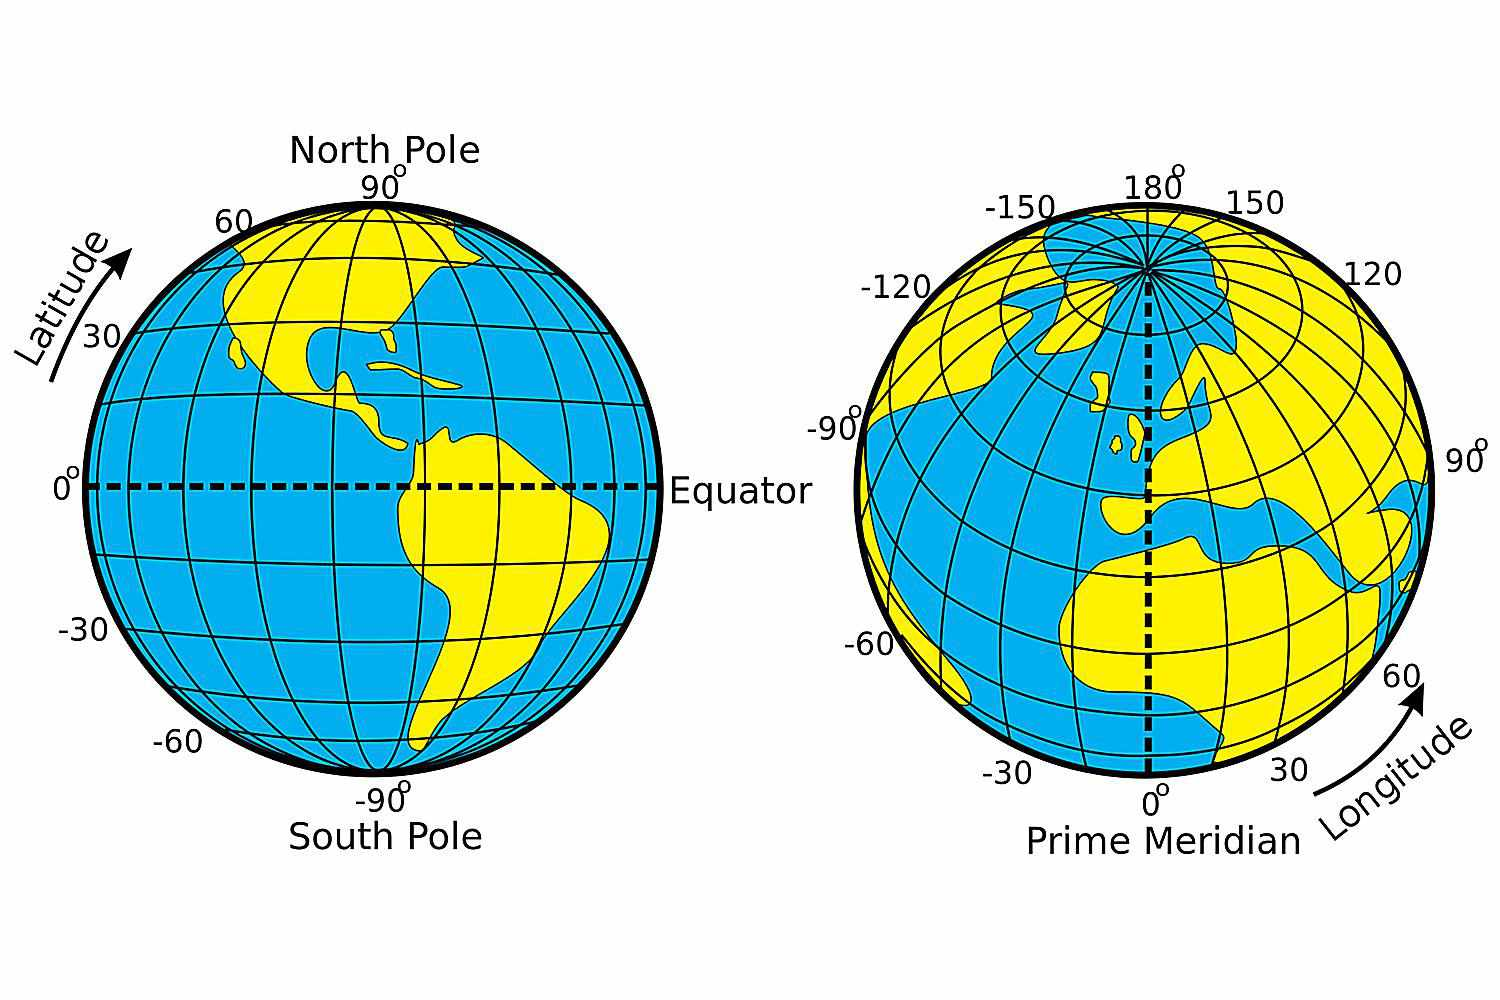
\includegraphics[width=0.5\textwidth]{C:/Users/Matteo/Shallow-Water-Equations/figs/lat-long-earth.jpg}
    \caption{Illustration of latitude and longitude on the planet earth.
    Illustration from~\cite{lat-long-earth}.}\label{fig:lat-long-earth}
\end{figure}
From \autoref{fig:lat-long-earth}, we see that the latitude direction is the north-south component, whereas the longitude direction is the east-west component.
The latitude angle, denoted by $\phi$, goes from $-\frac{\pi}{2}$ radians at the south pole to $\frac{\pi}{2}$ radians at the north pole, and the longitude angle, denoted by $\theta$, goes from $0$ at the prime meridian through Europe and western Africa, increasing to the east, to $2\pi$ radians.
The spherical coordinates we use are ($r$, $\theta$, $\phi$), where $r$ is the radius from the center of the sphere, $\theta$ is the longitude angle, and $\phi$ is the latitude angle. Both angles are measured in radians.
This also means, that any point on the surface of the sphere can be represented by the coordinates ($\theta$, $\phi$), since we assume the radius $r$ is constant.
We consider a small domain of the sphere, as illustrated in \autoref{fig:sphere-small-domain}.
\begin{figure}[H]
    \centering
    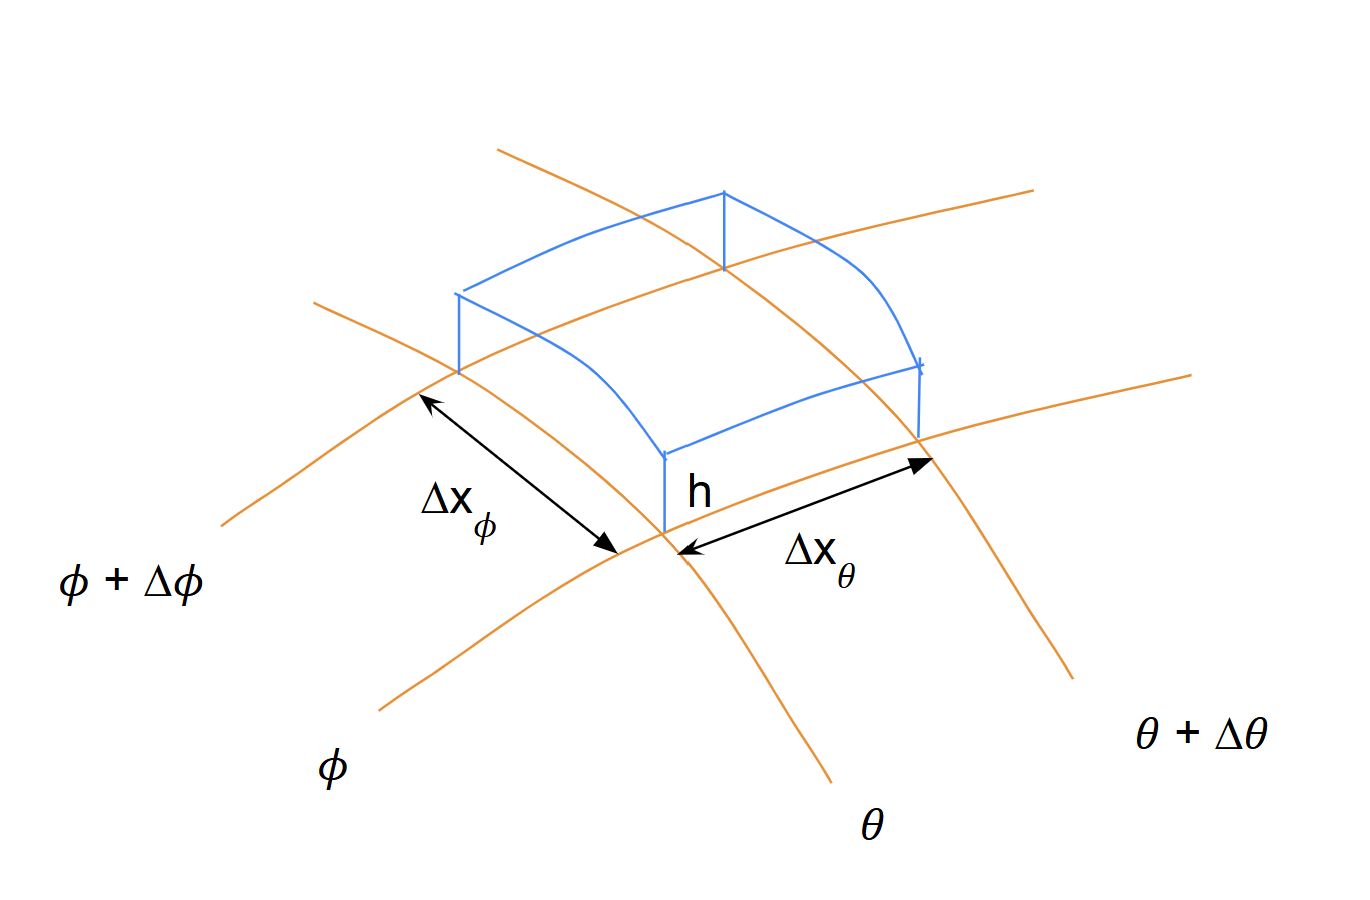
\includegraphics[width=0.5\textwidth]{C:/Users/Matteo/Shallow-Water-Equations/figs/Sphere-small-domain.png}
    \caption{Illustrations of a small domain of the surface of the sphere.}\label{fig:sphere-small-domain}
\end{figure}
The volume of the domain in~\autoref{fig:sphere-small-domain} is denoted by $V$.
We want to find expressions for $\Delta x_{\phi}$ and $\Delta x_{\theta}$, the distances in the $\phi$ and $\theta$ directions, respectively, as illustrated in \autoref{fig:sphere-small-domain}.
We can find these distances by using the arc length formula.
Recall that the circumreference of a full circle is $2\pi r$, where $r$ is the radius of the circle.
The arc length is a fraction of the full circumreference, and it is given by the formula $l = r v$, where $l$ is the arc length, $r$ is the radius, and $v$ is the angle in radians.
Assuming Earth's latitude side is a circle, we can find the distance $\Delta x_{\phi}$ by using the arc length formula, as:
\begin{align*}
    \Delta x_{\phi} = r \Delta \phi,
\end{align*}
where $\Delta \phi$ is the change in the latitude angle and $r$ is the radius of the sphere.
We assume that Earth is a perfect sphere, meaning that the radius is constant.
Considering the distance in the longitude dimension $\Delta x_{\theta}$, we need to make some adjustments, as we can see that the circumreference at equator is larger than at the poles.
That is, we need to consider the radius of the circle at the given latitude $\phi$.
To illustrate this, we consider \autoref{fig:sphere_r_lat}.
\begin{figure}[H]
    \centering
    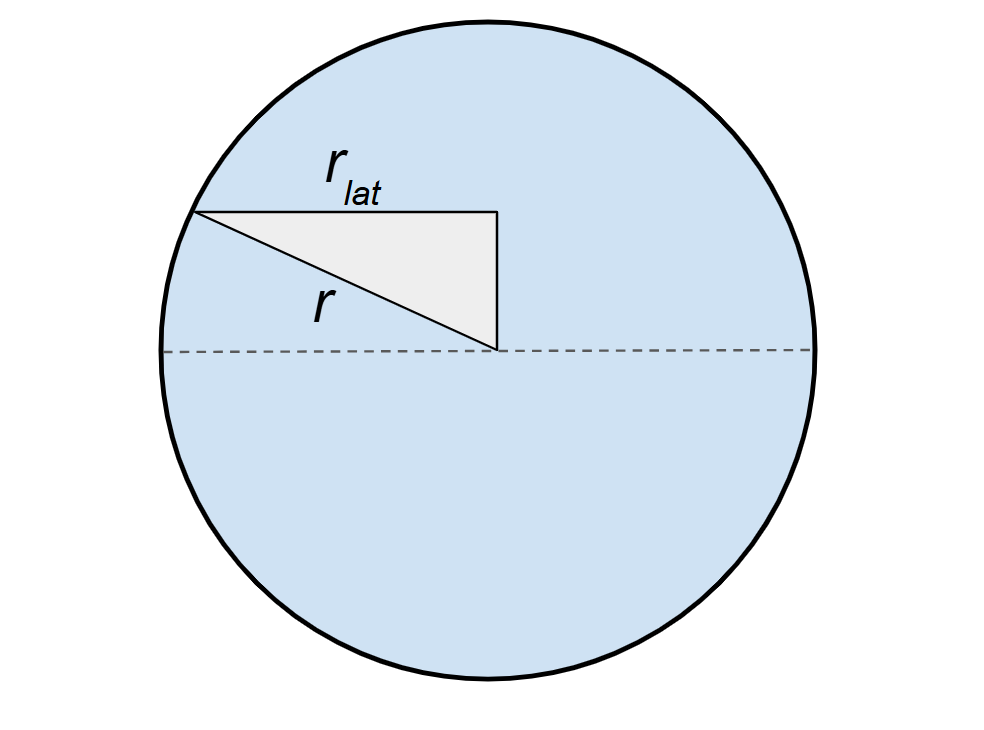
\includegraphics[width=0.4\textwidth]{C:/Users/Matteo/Shallow-Water-Equations/figs/sphere_r_lat.png}
    \caption{Illustration of the radius of the circle at the given latitude $\phi$.}\label{fig:sphere_r_lat}
\end{figure}
In \autoref{fig:sphere_r_lat}, we consider a right triangle where the length of the hypotenuse is equal to the radius of the sphere.
The length of the adjacent side $r_{lat}$ is the radius of the longitude circle at the given latitude $\phi$.
By using trigonometry, we can express the radius of the circle at the given latitude $\phi$ as
\begin{align*}
    r_{lat} = r \cos(\phi).  
\end{align*}
Using that, together with the arc length formula, we can find the distance $\Delta x_{\theta}$ as:
\begin{align*}
    \Delta x_{\theta} = r \cos(\phi) \Delta \theta.
\end{align*}
We can then compute the volume of a small domain of the sphere, as shown in \autoref{fig:sphere-small-domain}.
The volume $V$ is given by 
\begin{align*}
    V &= \Delta x_{\phi} \Delta x_{\theta} h \\
    &= r^2 h \cos(\phi) \Delta \phi \Delta \theta,
\end{align*}
assuming that the height of the domain is $h$, and that the domain is rectangular.
This is a fair assumption for small values of $\Delta x_{\phi}$ and $\Delta x_{\theta}$.
We also assume that $\phi$ is not too close to the poles, as $\cos(\phi)$ will go to zero at the poles.
We are interested in the rate of change of $V$ with respect to time, and we can find this by taking the time derivative of the volume.
That is, we consider the partial derivative with respect to time of the volume $V$:
\begin{align}\label{eq:sphere-volume-time-derivative}
    \frac{\partial V}{\partial t} &= r^2 \cos(\phi) \Delta \phi \Delta \theta \frac{\partial h}{\partial t}.
\end{align}
In~\eqref{eq:sphere-volume-time-derivative} we have utilized that $r$ is constant, and that $\cos(\phi), \Delta \phi$ and $\Delta \theta$ are independent of the time $t$.
We use $u_{\theta}$ and $u_{\phi}$ to denote the velocities in the $\theta-$ and $\phi-$directions.
We are interested in the rate at which fluid volume enters the region from the sides.
We can find this rate by considering the flux of fluid volume through the sides of the domain.
That is, we consider how much fluid volume enters the domain from the $\theta-$direction, and how much fluid volume enters the domain from the $\phi-$direction.
We also consider how much fluid volume leaves the domain in the $\theta-$ and $\phi-$directions.
The net flux of fluid volume into the domain is the difference between the influx and the outflux.
The rate of change of the volume $V$ with respect to time is equal to the net flux of fluid volume into the domain.
That is, we have that
\begin{align}\label{eq:V_t-F_net}
    V_t = F_{net, \theta} + F_{net, \phi},
\end{align}
which combined with~\eqref{eq:sphere-volume-time-derivative} gives us the equation
\begin{align}\label{eq:sphere-volume-time-combined}
    r^2 \cos(\phi) \Delta \phi \Delta \theta \frac{\partial h}{\partial t} = F_{net, \theta} + F_{net, \phi}.
\end{align}
To find the net flux in the $\theta$ and $\phi$ directions, we consider the influx and outflux in these directions.
We calculate the influx at the $\theta-$line and the outflux at $(\theta + \Delta \theta)-$line, see \autoref{fig:sphere-small-domain}, to find the net flux.
The influx is the area of the $\theta$ line times the velocity in the $\theta$ direction at the $\theta$ line.
The influx in the $\theta$-direction is given by
\begin{align*}
    F_{in, \theta} = u_\theta(\theta) h(\theta)  r \Delta \phi,
\end{align*}
where $h(\theta)$ is the height of the water at the $\theta-$line, assumed to be constant along the line, and $u_\theta(\theta)$ is the velocity in the $\theta-$direction at the $\theta-$line.
This way we can compute how much the volume changes due to the influx.
For the outflux we do the same just for the $\theta + \Delta \theta$ line, introducing the notation $\theta ' = \theta + \Delta \theta$.
The outflux is
\begin{align*}
    F_{out, \theta}
    = u_\theta(\theta + \Delta \theta) h(\theta + \Delta \theta)  r \Delta \phi
    = u_\theta(\theta') h(\theta')  r \Delta \phi
    .
\end{align*}
The net flux in the $\theta$ direction is the difference between the influx and the outflux, and is given by
\begin{align}\label{eq:sphere-net-flux-theta}
   F_{net, \theta} = F_{in, \theta} - F_{out, \theta} 
    = \left(  u_\theta(\theta) h(\theta) - u_\theta(\theta ') h(\theta ') \right)  r \Delta \phi.
\end{align}
We can do the same for the $\phi$ direction, also using the notation $\phi ' = \phi + \Delta \phi$.
Hence, we obtain the net flux in the $\phi$ direction as
\begin{align}\label{eq:sphere-net-flux-phi}
    F_{net, \phi} &= F_{in, \phi} - F_{out, \phi} \\
     &= \left( u_\phi(\phi) h(\phi)\cos (\phi) - u_\phi (\phi ')h(\phi ') \cos(\phi')  \right) r \Delta \theta.
\end{align}
By inserting~\eqref{eq:sphere-net-flux-theta} and~\eqref{eq:sphere-net-flux-phi} into~\eqref{eq:sphere-volume-time-combined} we can write:
\begin{align}\label{eq:sphere-volume-time-derivative-flux}
    h_t r^2 \cos(\phi) \Delta \phi \Delta \theta
    = \left( u_\theta(\theta) h(\theta) - u_\theta (\theta ')h(\theta ')  \right) r \Delta \phi
    + \left( u_\phi(\phi) h(\phi)\cos (\phi) - u_\phi (\phi ')h(\phi ') \cos(\phi')  \right) r \Delta \theta.
\end{align}
Since we are interested in $\frac{\partial h}{\partial t} = h_t$, we divide~\eqref{eq:sphere-volume-time-derivative-flux} by the area of the element $r^2 \cos(\phi) \Delta \phi \Delta \theta$.
Hence we get
\begin{align}\label{eq:sphere-derivative-h}
    \frac{\partial h}{\partial t} = \frac{u_\theta(\theta) h(\theta) - u_\theta(\theta ')h(\theta ') }{r \cos(\phi) \Delta \theta} 
    + \frac{u_\phi(\phi) h(\phi)\cos (\phi) - u_\phi (\phi ')h(\phi ') \cos(\phi')}{r \cos (\phi) \Delta \phi},
\end{align}
where $\phi \neq \pm \frac{\phi}{2}$.
By collecting terms to the left hand side and changing the order of the numerators, we can rewrite~\eqref{eq:sphere-derivative-h} as 
\begin{align}\label{eq:sphere-derivative-h-collected}
    \frac{\partial h}{\partial t} + \frac{u_\theta(\theta') h(\theta') - u_\theta(\theta)h(\theta) }{r \cos(\phi) \Delta \theta} 
    + \frac{u_\phi(\phi ')h(\phi ') \cos(\phi') - u_\phi(\phi) h(\phi) \cos(\phi) }{r \cos (\phi) \Delta \phi} = 0.
\end{align}
Next step is to investigate the limit values, as $\Delta \theta$ and $\Delta \phi$ goes to zero.
We can find the limit values by using the definition of the derivative.
The derivative of a function $f$ with respect to $x$ is defined as
\begin{align*}
    f'(x) = \lim_{\Delta x \to 0} \frac{f(x + \Delta x) - f(x)}{\Delta x}.
\end{align*}
We can use this definition to find the limit values in~\eqref{eq:sphere-derivative-h-collected}.
\begin{align*}
    \lim_{\Delta \theta \to 0} \frac{ u_\theta(\theta ')h(\theta ') - u_\theta(\theta) h(\theta) }{\Delta \theta} = \frac{\partial}{\partial \theta} (h u_\theta ),
\end{align*}
and 
\begin{align*}
    \lim_{\Delta \phi \to 0} \frac{ u_\phi(\phi ')h(\phi ') \cos(\phi') - u_\phi(\phi) h(\phi) \cos(\phi) }{\Delta \phi} =  \frac{\partial}{\partial \phi} (h u_\phi \cos(\phi)).
\end{align*}
Inserting these results in~\eqref{eq:sphere-derivative-h-collected} yields
\begin{align*}
    h_t + \frac{1}{r \cos (\phi)} \left( {(h u_\theta)}_{\theta} + {(h u_{\phi} \cos(\phi))}_{\phi}  \right) = 0,
\end{align*}
which is the mass conservation equation in spherical coordinates and is the first equation in the shallow water equations in spherical coordinates.
The next step is to derive the momentum equations in spherical coordinates.
In this case, we focus on the horizontal velocity components, specifically the velocity tangential to the surface of the sphere, i.e., the $\theta$ and $\phi$ velocities.
The vertical velocity is neglected, as the key assumption in the shallow water equations is that the vertical component of the acceleration is negligible.
Additionally, when considering Earth, the water layer is thin compared to the radius of the Earth, referred to as a thin-layer approximation.
We need to express the horizontal velocity $u_h$, which is dependent on the variables $\theta, \phi$ and $t$.
Since $\theta$ and $\phi$ are angles, we introduce the unit vectors $\mathbf{e}_\theta$ and $\mathbf{e}_\phi$ on the surface in the $\theta-$ and $\phi-$directions.
The unit vectors are illustrated in~\autoref{fig:sphere-unit-vectors}.
\begin{figure}[H]
    \centering
    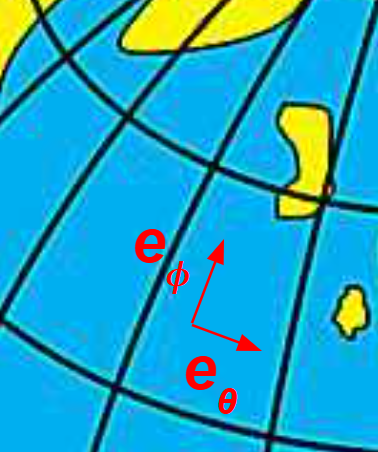
\includegraphics[width=0.2\textwidth]{C:/Users/Matteo/Shallow-Water-Equations/figs/sphere-unit-vectors.png}
    \caption{Illustration of the unit vectors $\mathbf{e}_\theta$ and $\mathbf{e}_\phi$, tangential to the surface.}\label{fig:sphere-unit-vectors}
\end{figure}
We can express the horizontal velocity $u_h$ in terms of the unit vectors as
\begin{align}\label{eq:sphere-horizontal-velocity}
    u_h(\theta, \phi, t) = u_\theta \mathbf{e}_\theta + u_\phi \mathbf{e}_\phi.
\end{align}
We are then interested in the total derivative of the horizontal velocity $u_h$ in~\eqref{eq:sphere-horizontal-velocity} with respect to time.
The total derivative is given by
\begin{align}\label{eq:sphere-total-derivative}
    \frac{\text{d}u_h}{\text{d}t} = \frac{\partial u_h}{\partial t} + \frac{\text{d}\theta}{\text{d}t} \frac{\partial u_h}{\partial \theta} + \frac{\text{d}\phi}{\text{d}t} \frac{\partial u_h}{\partial \phi}.
\end{align}
If we differentiate the longitude angle $\theta$ with respect to time, we get the angular velocity $\omega_\theta$ in the $\theta$ direction, i.e.,
\begin{align*}
    \frac{\text{d}\theta}{\text{d}t} = \omega_\theta,
\end{align*}
meaning that if $\omega_\theta > 0$, the point is moving eastwards, and if $\omega_\theta < 0$, the point is moving westwards.
Similarly, if we differentiate the latitude angle $\phi$ with respect to time, we get the angular velocity $\omega_\phi$ in the $\phi$ direction, i.e.,
\begin{align*}
    \frac{\text{d}\phi}{\text{d}t} = \omega_\phi,
\end{align*}
meaning that if $\omega_\phi > 0$, the point is moving northwards, and if $\omega_\phi < 0$, the point is moving southwards.
By using the  derivative of the arc length formula, we get that 
\begin{align}\label{eq:sphere-arc-length}
    \frac{\text{d}\theta}{\text{d}t} =  \frac{u_\theta}{r \cos(\phi)},
    \quad \frac{\text{d}\phi}{\text{d}t} = \frac{u_\phi}{r}.
\end{align}
We can now insert~\eqref{eq:sphere-arc-length} into~\eqref{eq:sphere-total-derivative} to find the total derivative of the horizontal velocity split into the $\theta$ and $\phi$ directions:
\begin{equation}\label{eq:sphere-total-derivative-split}
    \left.
    \begin{aligned}
        \frac{\text{d}u_\theta}{\text{d}t} = \frac{\partial u_\theta}{\partial t} + \frac{u_\theta}{r \cos(\phi)} \frac{\partial u_\theta}{\partial \theta} + \frac{u_\phi}{r} \frac{\partial u_\theta}{\partial \phi}, \\
        \frac{\text{d}u_\phi}{\text{d}t} = \frac{\partial u_\phi}{\partial t} + \frac{u_\theta}{r \cos(\phi)} \frac{\partial u_\phi}{\partial \theta} + \frac{u_\phi}{r} \frac{\partial u_\phi}{\partial \phi}.
    \end{aligned}
    \right\}
\end{equation}
We know that the right hand side of~\eqref{eq:sphere-total-derivative-split} are the given physical forces acting on the fluid.
Earlier in this project, we focused on the shallow water equations in cartesian coordinates, accounting solely for gravitational forces.
However, in spherical coordinates, additional physical forces must be considered. These include the Coriolis force, centripetal acceleration, and the effects of Earth's curvature.
First we consider the gravitational force acting on the fluid, descibed as $-g \Delta h$, where $g$ is the gravitational constant, and $\Delta h$ is the gradient of the height $h$.
We consider the gradient of $h(\theta, \phi)$:
\begin{align}
    \Delta h  &= \frac{1}{r \cos(\phi)} h_{\theta} \mathbf{e}_{\theta} + \frac{1}{r } h_{\phi} \mathbf{e}_{\phi},
\end{align}
meaning that the gravity force acting on the fluid in the $\theta$ and $\phi$ directions are given by:
\begin{align*}
    &\theta-\text{direction:} \quad -\frac{g}{r \cos(\phi)} h_{\theta},\\
    &\phi-\text{direction:} \quad -\frac{g}{r} h_{\phi}.
\end{align*}
Hence, we obtain the two momentum equations in spherical coordinates as
\begin{equation}
    \begin{aligned}
         {(u_\theta)}_t + \frac{u_\theta}{r \cos(\phi)} {(u_\theta)}_\theta + \frac{u_\phi}{r} {(u_\theta)}_\phi = -\frac{g}{r \cos(\phi)} h_{\theta} + \text{other forces}, \\
        {( u_\phi)}_t + \frac{u_\theta}{r \cos(\phi)} {(u_\phi)}_\theta   + \frac{u_\phi}{r} {(u_\phi)}_\phi = -\frac{g}{r} h_{\phi} + \text{other forces}.
    \end{aligned}
\end{equation}
The next force we consider is the Coriolis force, which is a force that acts on moving objects on the surface of the earth~\cite{Coriolis}.
The Coriolis force is given by $f = 2 \Omega \sin(\phi)$, where $\Omega$ is the angular velocity of the earth.
The Coriolis force in the $\theta$ and $\phi$ directions are then given by:
\begin{align*}
   &\theta-\text{direction:} \quad f u_\phi,\\
    &\phi-\text{direction:} \quad -f u_\theta.
\end{align*}
The last thing we need to take into account when working in the spherical domain is the curvature of the earth.
This adds the following terms:
\begin{align*}
    &\theta-\text{direction:} \quad \frac{u_\theta u_\phi}{r} \tan(\phi),\\
    &\phi-\text{direction:} \quad -\frac{u_\theta^2}{r} \tan(\phi).
\end{align*}

There are several formulations of the SWE in spherical coordinates.
Inserting these forces into the momentum equations, we get the following formulation of the shallow water equations in spherical coordinates:
\begin{equation}
    \left.
    \begin{aligned}
        h_t + \frac{1}{r \cos (\phi)} \left( {(h u_\theta)}_{\theta} + {(h u_{\phi} \cos(\phi))}_{\phi}  \right) &= 0, \\
        {(u_{\theta})}_t  + \frac{u_\theta}{r \cos (\phi)} {(u_\theta)}_\theta + \frac{u_\phi}{r} {(u_\theta)}_{\phi}
        - \frac{u_\theta u_\phi }{r} \tan(\phi) + \frac{g}{r \cos (\phi)} h_\theta - f u_\phi &= 0, \\
        {(u_{\phi})}_t  + \frac{u_\theta}{r \cos (\phi)} {(u_\phi)}_\theta + \frac{u_\phi}{r} {(u_\phi)}_{\phi}
        + \frac{u_\theta^2}{r} \tan(\phi) + \frac{g}{r} h_\phi + f u_\theta &= 0,
    \end{aligned}
    \right\}
\end{equation}
where $r$ is the radius, $(\theta, \phi)$ are the longitude and latitude angles, $h$ is the height of the water, $u_\theta$ and $u_\phi$ are the velocities in the $\theta$ and $\phi$ directions, $g$ is the gravitational constant.

%Obtain in vector form:
%Multiply with $\cos \phi$ and something else. Consider the paper.

%Vector form:
%\begin{align}
%    \cos(\phi) \mathbf{U}_t + \mathbf{F(U)}_\theta + \cos(\phi) \mathbf{G(U)}_\phi = 0,
%\end{align}
%where 
%\begin{align*}
%    \mathbf{U} = \begin{bmatrix} h \\ h u_\theta \\h u_\phi \end{bmatrix},
%    \mathbf{F(U)} = \begin{bmatrix} h u_\theta \\ h u_\theta^2 + g h^2  \\ h u_\theta u_\phi \end{bmatrix},
%    \mathbf{G(U)} = \begin{bmatrix} h u_\phi \\ h u_\theta u_\phi \\ h u_\phi^2 + \ g h^2 \end{bmatrix}.
%\end{align*}



\section{Linearized SWE in Spherical Coordinates}
In this section, we derive the linearized shallow water equations (SWE) in spherical coordinates, focusing on one spatial dimension, the longitude ($\theta$), and time ($t$).
This approach assumes a constant latitude ($\phi$), simplifying the equations to a one-dimensional framework.
The linearized SWE are employed for their simplicity, providing a foundation for understanding wave dynamics in a spherical geometry.
Later in this project, we will apply the finite volume method to solve these equations numerically.
The derivation and methodology presented here are based on the sources~\cite{BONEV_2018} and~\cite{Eskilsson_2005}.
We neglect all body forces other than gravity.
We linearize by assuming that the height of the water $h$ and the velocities $u$ are small perturbations from a state of rest.
We set $h = h_0 + h'$, $u = u_0 + u'$, where $h_0$ and $u_0$ are the equilibrium height and velocity, respectively, and $h'$ and $u'$ are the perturbations.
We also assume that the equilibrium height $h_0$ is constant.
To linearize the equations, we assume small perturbations around a mean state. Let the perturbations in water height and velocity be represented by:

\[
h = h_0 + h', \quad u_\theta = u'_\theta, \quad u_\phi = u'_\phi,
\]
where \( h_0 \) is the mean water height, and \( h' \), \( u'_\theta \), and \( u'_\phi \) represent the perturbations in the water height and velocity components, respectively.
Substituting these perturbed variables into the original equations and neglecting second-order terms (i.e., terms that involve products of perturbations), we obtain the following linearized shallow water equations:
\begin{equation}\label{eq:linearized_swe_spherical}
    \left.
    \begin{aligned}
        h'_t + \frac{h_0}{r \cos(\phi)} u'_\theta &= 0, \\
        u'_t + \frac{g}{r \cos(\phi)} h'_\theta &= 0.
    \end{aligned}
    \right\}
\end{equation}
These equations describe the evolution of small perturbations in water height and velocity on a spherical surface.
%Hence, we obtain the linearized shallow water equations in spherical coordinates with one spatial dimension ($\theta$) and time ($t$) as
We can also write the linearized shallow water equations in spherical coordinates in vector form as
\begin{align}\label{eq:linearized_swe_spherical_vector}
    \mathbf{W}_t + \mathbf{A} \mathbf{W}_\theta = 0,
\end{align}
where $\mathbf{W} =
\begin{bmatrix} h' \\ u' \end{bmatrix}$ and the coefficient matrix $\mathbf{A}$ is constant and given as:
$\mathbf{A} = \begin{bmatrix} 0 & \frac{h_0}{r \cos(\phi)} \\ \frac{g}{r \cos (\phi)} & 0 \end{bmatrix}$.


\subsubsection*{Integral form of the 1D spherical LSWE}
As we consider the longitude $\theta$ as the spatial dimension, the domain is the circle $[0, 2\pi]$, which is divided into $N$ cells or control volumes, each of length $\Delta \theta = \frac{2\pi}{N}$.
Each cell $i$ has a cell center at $\theta_i$ and cell boundaries/interfaces at $\theta_{i-1/2}$ and $\theta_{i+1/2}$.
\begin{figure}[H]
    \centering
    \begin{subfigure}{0.4\textwidth}
        \centering
        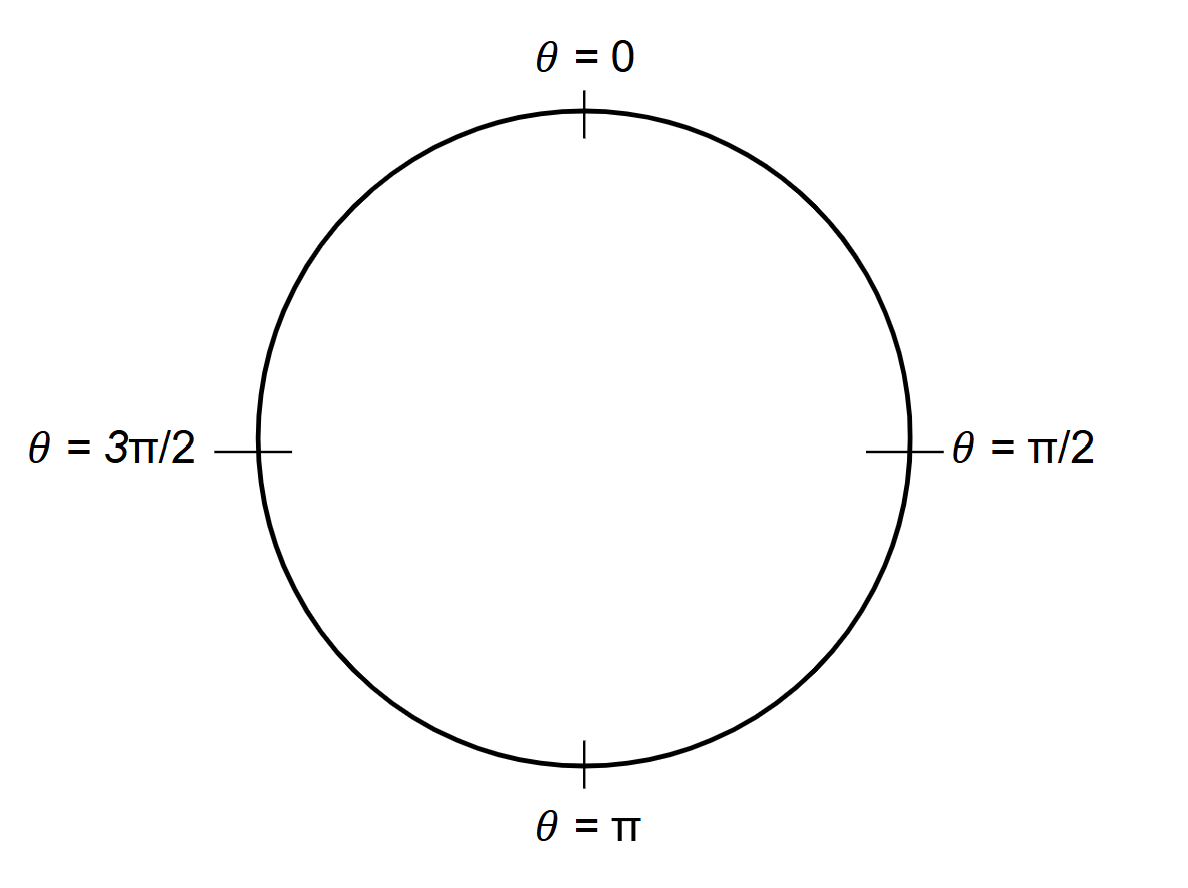
\includegraphics[width=\textwidth]{C:/Users/Matteo/Shallow-Water-Equations/figs/sphere1d_small_cell.png}
        \caption{Illustration of the grid for the 1D SWE with small cells.}\label{fig:sphere1d_small_cell}
    \end{subfigure}%
    \begin{subfigure}{0.35\textwidth}
        \centering
        \raisebox{10mm}{
        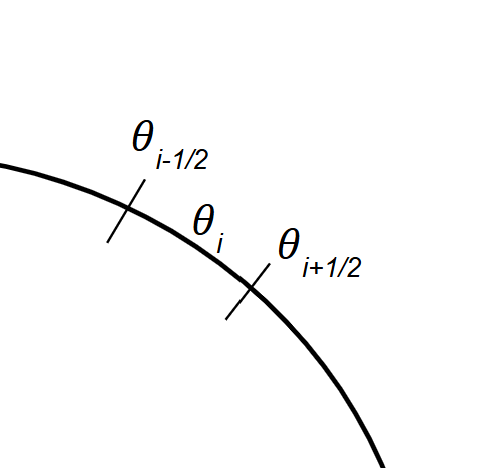
\includegraphics[width=0.9\textwidth]{C:/Users/Matteo/Shallow-Water-Equations/figs/sphere-1d-small-domain.png}
        }
        \caption{Illustration of the grid for the 1D SWE with a small domain.}\label{fig:sphere1d_small_domain}
    \end{subfigure}
    \caption{Grid illustrations for the 1D SWE in spherical coordinates.}\label{fig:sphere1d_combined}
\end{figure}
As when deriving the finite volume scheme for the 1D SWE in cartesian coordinates, we start by integrating the linearized shallow water equations over the control volume, and then divide by the cell length to obtain the finite volume scheme.
We integrate the vector form of the 1D SWE in spherical coordinates without the coriolis force over $\theta$ from $\theta_L := \theta_i - \frac{1}{2} \Delta \theta $ to $\theta_R := \theta_i + \frac{1}{2}\Delta \theta $ to obtain
\begin{align*}
    \int_{\theta_L}^{\theta_R} \mathbf{W}_t \text{ d}\theta + \int_{\theta_L}^{\theta_R} \mathbf{A} \mathbf{W}_\theta \text{ d}\theta = 0.
\end{align*}
Since the matrix $\mathbf{A}$ is constant, we can take it out of the integral:
\begin{align*}
    \int_{\theta_L}^{\theta_R} \mathbf{W}_t \text{ d}\theta + \mathbf{A} \int_{\theta_L}^{\theta_R} \mathbf{W}_\theta \text{ d}\theta = 0.
\end{align*}
We also use the fundamental theorem of calculus to rewrite the integral of the derivative as the difference of the function at the boundaries:
\begin{align}\label{eq:derive_integral_form_1D_spherical}
    \int_{\theta_L}^{\theta_R} \mathbf{W}_t \text{ d}\theta =  \mathbf{A} \left( \mathbf{W}(\theta_L, t) - \mathbf{W}(\theta_R, t) \right).
\end{align}
We can also write the equations out to get a better understanding of the terms:
\begin{equation}\label{eq:integral_form_spherical_1D}
    \left.
    \begin{aligned}
        \frac{\partial}{\partial t} \int_{\theta_L}^{\theta_R} h \text{ d}\theta + \frac{h_0}{r \cos(\phi)} (u_R - u_L) &= 0, \\
        \frac{\partial}{\partial t} \int_{\theta_L}^{\theta_R} u \text{ d}\theta + g(h_R - h_L) + fu_i &= 0.
    \end{aligned}
    \right\}
\end{equation}
Then we integrate~\eqref{eq:derive_integral_form_1D_spherical} over time from $t_1 := t_n$ to $t_2 := t_{n+1}$:
\begin{align*}
    \int_{t_1}^{t_2} \int_{\theta_L}^{\theta_R} \mathbf{W}_t \text{ d}\theta \text{ d}t = \mathbf{A} \left( \int_{t_1}^{t_2} \mathbf{W}(\theta_L, t) \text{ d}t - \int_{t_1}^{t_2} \mathbf{W}(\theta_R, t) \text{ d}t \right).
\end{align*}
Rewriting, using the fundamental theorem of calculus, gives
\begin{align}\label{eq:integral_form_spherical_1D_final}
    \int_{\theta_L}^{\theta_R} \mathbf{W}(\theta, t_2) \text{ d}\theta = \int_{\theta_L}^{\theta_R} \mathbf{W}(\theta, t_1) \text{ d}\theta
    - \mathbf{A} \left( \int_{t_1}^{t_2} \mathbf{W}(\theta_R, t) \text{ d}t - \int_{t_1}^{t_2} \mathbf{W}(\theta_L, t) \text{ d}t \right),
\end{align}
which we refer to as the integral form of the linearized shallow water equations in spherical coordinates with one spatial dimension and time.
The integral form~\eqref{eq:integral_form_spherical_1D_final} is the foundation for the finite volume method, which we will use to solve the linearized shallow water equations in spherical coordinates numerically.




\section{Finite Volume Method for the Shallow Water Equations}
In this section, we present the finite volume method (FVM) for solving nonlinear systems of balance laws, specifically focusing on the shallow water equations (SWE).
Nonlinear problems are more challenging than linear problems, as stability and convergence theory are more difficult.
Our focus is on discountinuous solutions, that can accurately capture shock waves and other discontinuities.
The approach described here is based on the work of LeVeque~\cite{LeVeque2002}.

In finite volume methods, the computational domain is discretized into cells or control volumes.
At the interfaces between these cells, we solve the local Riemann problem to compute the fluxes.
These fluxes are then used to update the solution in each cell.
By solving the Riemann problem at cell interfaces, the FVM can handle discontinuous solutions, making it particularly well suited for hyperbolic balance laws, such as the shallow water equations.

\subsection{Finite Volume Methods for the 1D SWE}
We begin by considering finite volume methods for the SWE in one space dimension.
In the FVM, we discretize the domain into finite control volumes or cells:
\begin{align*}
    V_i = [x_{i-1/2}, x_{i+1/2}] \times [t_n, t_{n+1}],
\end{align*}
where $\Delta x = x_{i+1/2} - x_{i-1/2}$ is the length of the cell and $\Delta t = t_{n+1} - t_n$ is the time step.
The cell $V_i^n$ is illustrated in Figure~\ref{fig:control_volume_V_i_n}.
\begin{figure}[H]
    \centering
    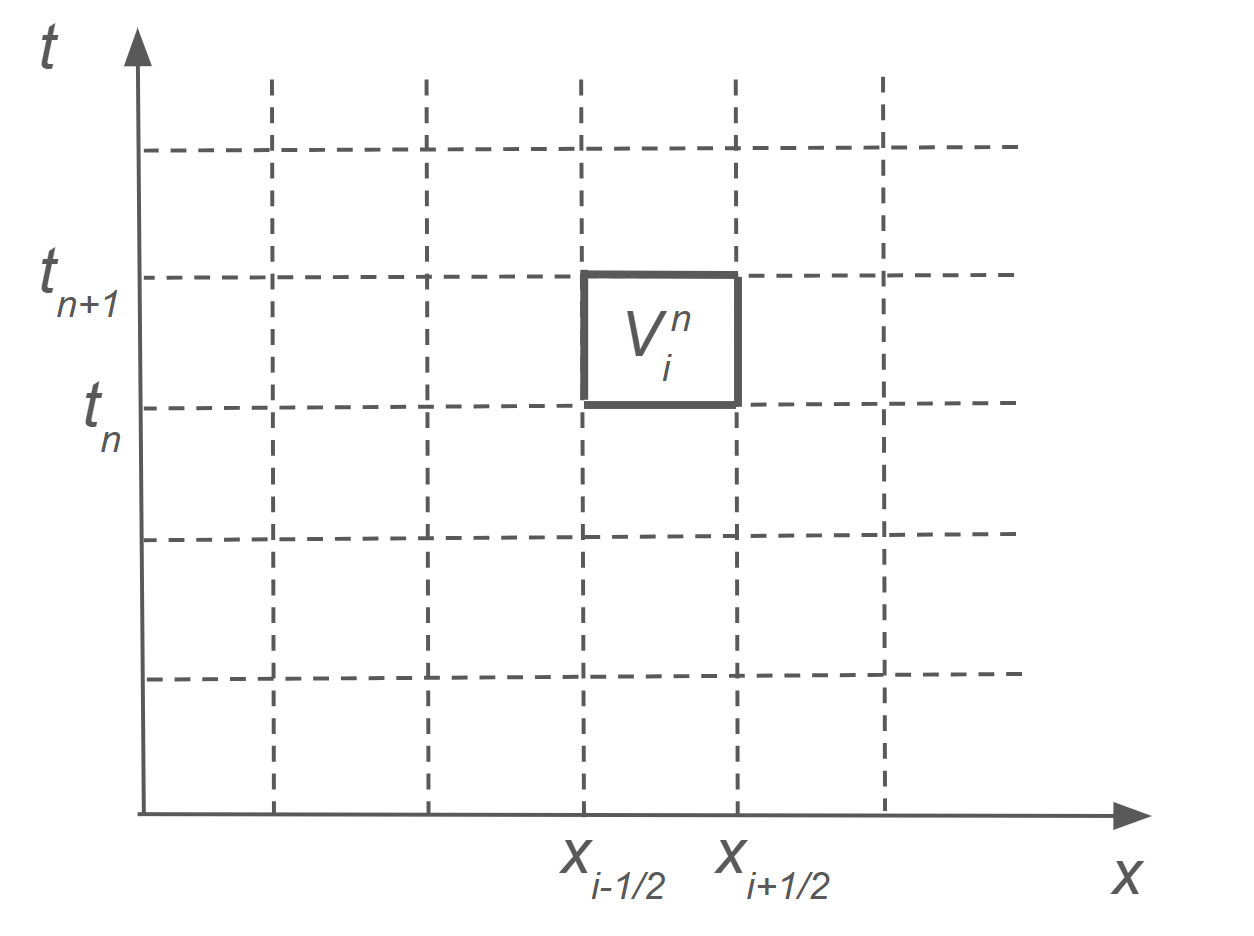
\includegraphics[width=0.4\textwidth]{C:/Users/Matteo/Shallow-Water-Equations/tex/figs/control_volume_V_i_n.png}
    \caption{Illustration of the control volume $V_i^n$ in the $x,t$ plane.}\label{fig:control_volume_V_i_n}
\end{figure}
For now, we will assume a uniform grid for simplicity.
The finite volume formula is derived from the integral form~\eqref{eq:integral_form_1D_final}.
By dividing the integral form of the 1D inhomoegeneous SWE by the cell length $\Delta x$, we espress it in terms of the newly defined cells:
\begin{align*}
    \frac{1}{\Delta x} \int_{x_{i-1/2}}^{x_{i+1/2}} \mathbf{U}(x,t_{n+1}) \text{ d}x &= \frac{1}{\Delta x} \int_{x_{i-1/2}}^{x_{i+1/2}} \mathbf{U}(x,t_n) \text{ d}x\\
    & - \frac{\Delta t}{\Delta x} \left[ \frac{1}{\Delta t} \int_{t_n}^{t_{n+1}} \mathbf{F}(\mathbf{U}(x_{i+1/2}, t)) \text{ d}t
    - \frac{1}{\Delta t} \int_{t_n}^{t_{n+1}} \mathbf{F}(\mathbf{U}(x_{i-1/2}, t)) \text{ d}t \right] \\
    &+ \frac{\Delta t}{\Delta x \Delta t} \int_{x_{i-1/2}}^{x_{i+1/2}} \int_{t_n}^{t_{n+1}} \mathbf{S(U)}(x,t) \text{d}x \text{d}t.
\end{align*}
For a finite volume $V_i^n$, averaging the terms over the volume yields the explicit conservative form
\begin{align}\label{eq:explicit_conservative_1D_SWE}
    \mathbf{U}_i^{n+1} = \mathbf{U}_i^n - \frac{\Delta t}{\Delta x} \left( \mathbf{F}_{i+1/2}^n - \mathbf{F}_{i-1/2}^n \right) + \Delta t \mathbf{S}_i.
\end{align}
The formula~\eqref{eq:explicit_conservative_1D_SWE} is referred to as a finite volume scheme.
The value $\mathbf{U}_i^n$ is the average value over the $i$-th cell at time $t_n$:
\begin{align}
    \mathbf{U}_i^n = \frac{1}{\Delta x} \int_{x_{i-1/2}}^{x_{i+1/2}} \mathbf{U}(x,t_n) \text{ d}x,
\end{align}
also known as the cell average.
The flux $\mathbf{F}_{i-1/2}^n$ is the average flux across the line $x = x_{i-1/2}$ from time $t_n$ to $t_{n+1}$:
\begin{align*}
    \mathbf{F}_{i-1/2}^n = \frac{1}{\Delta t} \int_{t_n}^{t_{n+1}} \mathbf{F}(\mathbf{U}(x_{i-1/2},t)) \text{ d}t,
\end{align*}
and correspondingly the flux $\mathbf{F}_{i+1/2}^n$ is the average flux across the line $x = x_{i+1/2}$ from time $t_n$ to $t_{n+1}$:
\begin{align*}
    \mathbf{F}_{i+1/2}^n = \frac{1}{\Delta t} \int_{t_n}^{t_{n+1}} \mathbf{F}(\mathbf{U}(x_{i+1/2},t)) \text{ d}t.
\end{align*}
The source term $\mathbf{S}_i$ is the average source term over the $i$-th cell at time $t_n$:
\begin{align*}
    \mathbf{S}_i &= \frac{1}{\Delta t \Delta x} \int_{t_n}^{t_{n+1}} \int_{x_{i-1/2}}^{x_{i+1/2}} \mathbf{S}(x,t) \text{ d}x\text{d}t.
\end{align*}
The values are illustrated in Figure~\ref{fig:10_3}.
\begin{figure}[H]
    \centering
    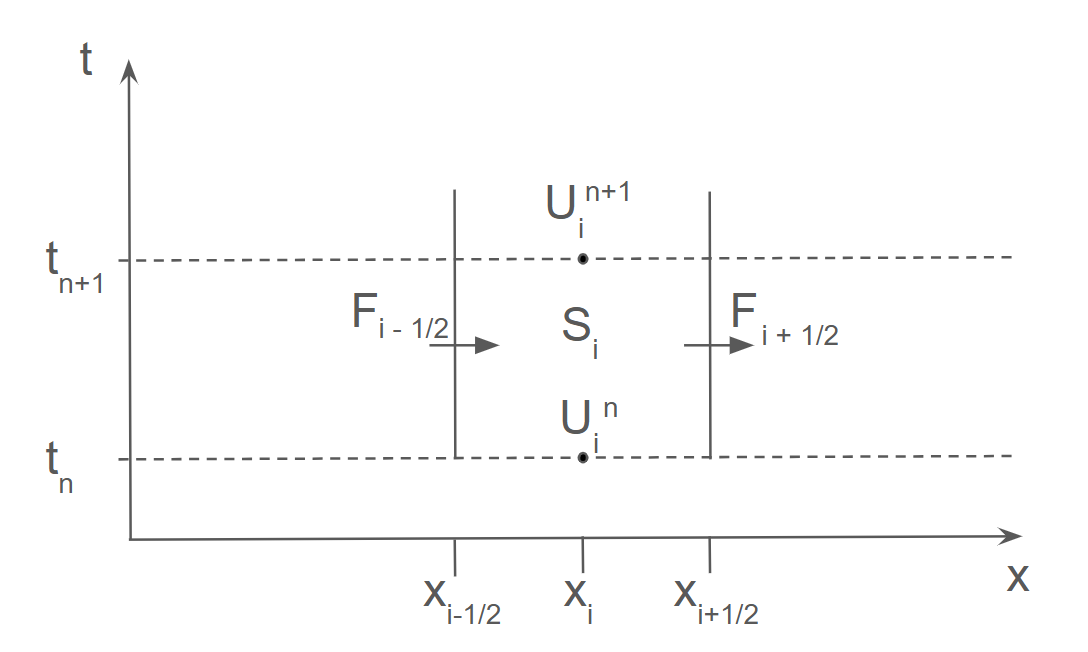
\includegraphics[width=0.5\textwidth]{C:/Users/Matteo/Shallow-Water-Equations/tex/figs/fvm_grid_new.png}
    \caption{Illustration of the grid for the 1D SWE.}\label{fig:10_3}
\end{figure}
The central idea of the FVM is to define the numerical flux $\mathbf{F}_{i+1/2}^n$, at the cell interface, as a function of the cell averages $\mathbf{U}_i^n$ and $\mathbf{U}_{i+1}^n$, since the solution is known only in terms of these cell averages.
Consequently, the FVM does not provide pointwise values of the solution, i.e., $\mathbf{U}(x,t)$, but instead gives cell-averaged values, $\mathbf{U}_i^n$, over the control volume.
One of the main challenges in the FVM is to determine appropiate numerical flux functions that, based on the available cell averages, can reasonably approximate the fluxes at the cell interfaces. 
Later in the thesis, we will consider several numerical flux functions that can be used to solve the local Riemann problem at the cell interfaces.

Finite volume methods are closely related to Finite Difference Methods (FDM), but they differs as they are based on the integral form of the conservation laws.
Where finite difference methods tend to break down near discontinuities in the solution, finite volume methods are more suited, since they are based on the integral form of the conservation laws.
The key distinction between the FVM and the FDM lies in their formulation: while the FVM is based on the integral conservation over finite volumes, the FDM is based on the differential conservation over finite differences.

\subsection{Finite Volume Method for the 2D SWE}
We now extend the FVM to two space dimensions.
Consider the 2D SWE in vector form~\eqref{eq:vector_form_2D} with $\mathbf{S(U)} = 0$:
\begin{align}\label{eq:2D_SWE}
    \mathbf{U}_t + \mathbf{F(U)}_x + \mathbf{G(U)}_y = 0.
\end{align}
Following the methods outlined in~\cite{Toro2009-Riemann}, an explicit finite volume scheme to solve~\eqref{eq:2D_SWE} is given by
\begin{align}
    \mathbf{U}_{i,j}^{n+1} = \mathbf{U}_{i,j}^n + \frac{\Delta t}{\Delta x}(\mathbf{F}_{i-1/2,j} - \mathbf{F}_{i+1/2,j}) + \frac{\Delta t}{\Delta y}(\mathbf{G}_{i,j-1/2} - \mathbf{G}_{i,j+1/2}).
\end{align}
This is the unsplit finite volume method, meaning that, in a single step, the cell average $\mathbf{U}_{i,j}^n$ is updated using the fluxes from all intercell boundaries.


\subsection{Finite Volume Method for the 1D SWE in spherical coordinates}
Simplified linearized shallow water equations on a circle. 
We consider the linearized shallow water equations in cartesian coordinates with one spatial dimension ($x$) and time ($t$).
\begin{equation}
    \left.
    \begin{aligned}
        h_t + H u_x = 0, \\
        u_t + g h_x = 0,
    \end{aligned}
    \right\}
\end{equation}
where $h$ is the height of the water, $u$ is the velocity of the water, $H$ is the average height of the water, and $g$ is the acceleration due to gravity.
We now consider the linearized shallow water equations in spherical coordinates with one spatial dimension, the longitude ($\theta$), and time ($t$).
That is, we assume constant latitude $\phi$. 
As we consider the longitude $\theta$ as the spatial dimension, the domain is the circle $[0, 2\pi]$, which is divided into $N$ cells or control volumes, each of length $\Delta \theta = \frac{2\pi}{N}$.
Each celle $i$ has a cell center at $\theta_i$ and cell boundaries/interfaces at $\theta_{i-1/2}$ and $\theta_{i+1/2}$.
\begin{figure}[H]
    \centering
    \begin{subfigure}{0.4\textwidth}
        \centering
        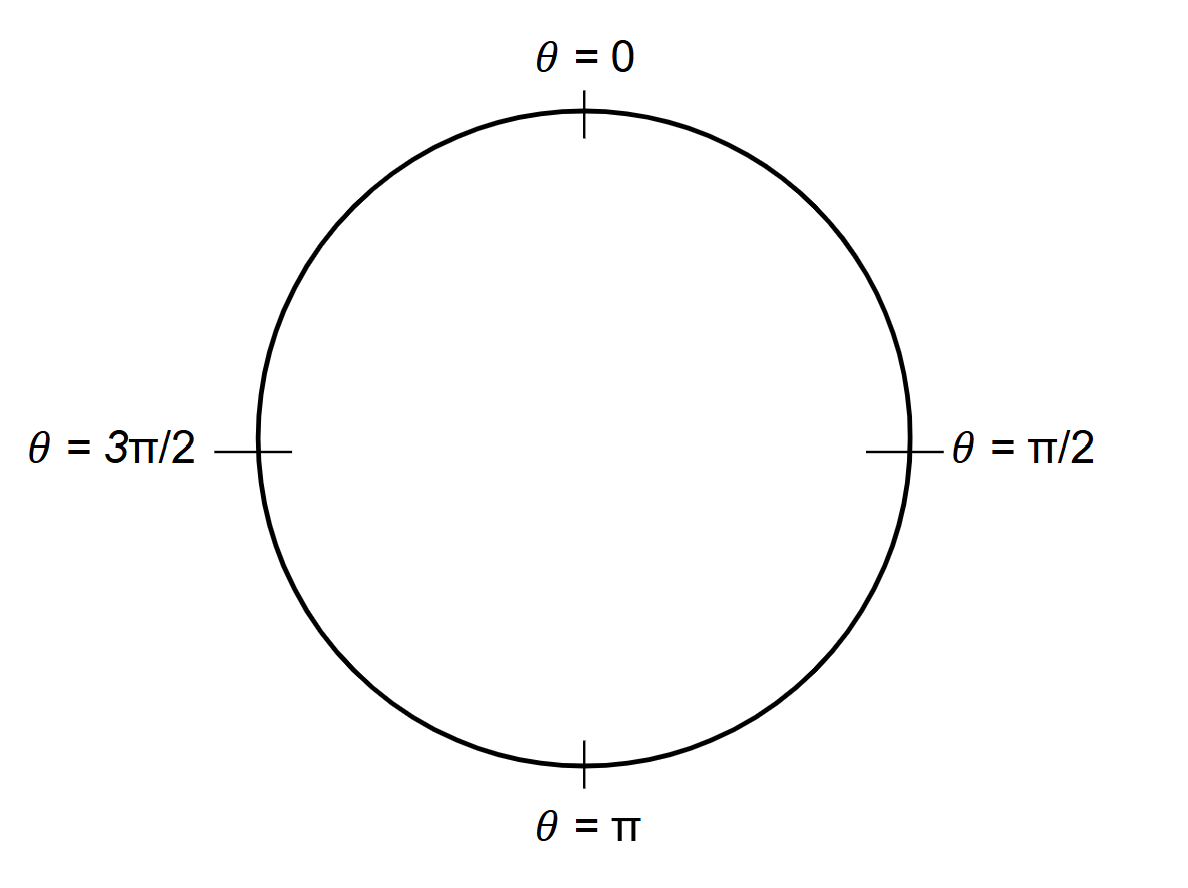
\includegraphics[width=\textwidth]{C:/Users/Matteo/Shallow-Water-Equations/figs/sphere1d_small_cell.png}
        \caption{Illustration of the grid for the 1D SWE with small cells.}\label{fig:sphere1d_small_cell}
    \end{subfigure}%
    \begin{subfigure}{0.35\textwidth}
        \centering
        \raisebox{10mm}{
        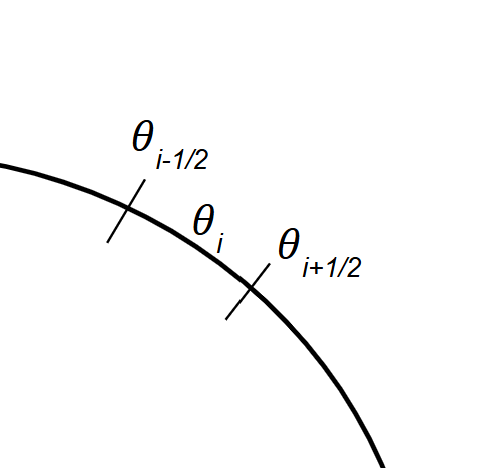
\includegraphics[width=0.9\textwidth]{C:/Users/Matteo/Shallow-Water-Equations/figs/sphere-1d-small-domain.png}
        }
        \caption{Illustration of the grid for the 1D SWE with a small domain.}\label{fig:sphere1d_small_domain}
    \end{subfigure}
    \caption{Grid illustrations for the 1D SWE in spherical coordinates.}\label{fig:sphere1d_combined}
\end{figure}

The linearized shallow water equations in spherical coordinates with one spatial dimension ($\theta$) and time ($t$) are given by
\begin{equation}\label{eq:linearized_swe_spherical}
    \left.
    \begin{aligned}
        h_t + \frac{H}{r \cos(\phi)} u_\theta = 0, \\
        u_t + g h_\theta + fu = 0,
    \end{aligned}
    \right\}
\end{equation}
where $r$ is the radius of the Earth, $\phi$ is the latitude, and $f$ is the Coriolis parameter.
We still refer to the equations as the mass and momentum equations, respectively.
We can also write the linearized shallow water equations in spherical coordinates in vector form, without the coriolis force, as
\begin{align}\label{eq:linearized_swe_spherical_vector}
    \mathbf{W}_t + \mathbf{A} \mathbf{W}_\theta = 0,
\end{align}
where $\mathbf{W} =
\begin{bmatrix} h \\ u \end{bmatrix}$ and the coefficient matrix $\mathbf{A}$ is constant and given as:
$\mathbf{A} = \begin{bmatrix} 0 & \frac{H}{r \cos(\phi)} \\ g & 0 \end{bmatrix}$.
We integrate the height equation in~\eqref{eq:linearized_swe_spherical} over $\theta$ from $\theta_L := \theta_i - \frac{1}{2} \Delta \theta $ to $\theta_R := \theta_i + \frac{1}{2}\Delta \theta $ to obtain
\begin{align*}
    \int_{\theta_L}^{\theta_R} h_t \text{ d}\theta + \int_{\theta_L}^{\theta_R} \frac{H}{r \cos(\phi)} u_\theta \text{ d}\theta = 0.
\end{align*}
The first term is 
\begin{align*}
    \frac{\partial}{\partial t} \int_{\theta_L}^{\theta_R} h \text{ d}\theta =  \Delta \theta h_t,
\end{align*}
meaning that the first term is the rate of change of the water height $h$ in the control volume.
The second term is
\begin{align*}
    \int_{\theta_L}^{\theta_R} \frac{H}{r \cos(\phi)} u_\theta \text{ d}\theta = \frac{H}{r \cos(\phi)} (u_R - u_L),
\end{align*}
where $u_R$ and $u_L$ are the velocities at the right and left boundaries of the control volume, respectively.
Then we integrate the momentum equation in~\eqref{eq:linearized_swe_spherical} over $\theta$ from $\theta_L$ to $\theta_R$ to obtain
\begin{align*}
    \int_{\theta_L}^{\theta_R} u_t \text{ d}\theta + \int_{\theta_L}^{\theta_R} g h_\theta \text{ d}\theta + \int_{\theta_L}^{\theta_R} fu \text{ d} \theta = 0.
\end{align*}
The first term gives the time rate of change in the velocity $u$ in the control volume:
\begin{align*}
    \frac{\partial}{\partial t} \int_{\theta_L}^{\theta_R} u \text{ d}\theta = \Delta \theta u_t.
\end{align*}
The second term gives 
\begin{align*}
    \int_{\theta_L}^{\theta_R} g h_\theta \text{ d}\theta = g(h_R - h_L),
\end{align*}
where $h_R$ and $h_L$ are the heights at the right and left boundaries of the control volume, respectively.
The third term with the Coriolis force gives
\begin{align*}
    \int_{\theta_L}^{\theta_R} fu \text{ d}\theta = f(u_R - u_L) \Delta \theta.
\end{align*} 
Hence, the integral form of the linearized shallow water equations in spherical coordinates with one spatial dimension and time is
\begin{equation}\label{eq:integral_form_spherical_1D}
    \left.
    \begin{aligned}
        \frac{\partial}{\partial t} \int_{\theta_L}^{\theta_R} h \text{ d}\theta + \frac{H}{r \cos(\phi)} (u_R - u_L) &= 0, \\
        \frac{\partial}{\partial t} \int_{\theta_L}^{\theta_R} u \text{ d}\theta + g(h_R - h_L) + fu_i &= 0.
    \end{aligned}
    \right\}
\end{equation}
Then we integrate~\eqref{eq:integral_form_spherical_1D} over time from $t_1:= t_n$ to $t_2:= t_{n+1}$:
\begin{equation}
    \begin{aligned}
        \int_{t_1}^{t_2} \int_{\theta_L}^{\theta_R} h_t \text{ d}\theta \text{d}t + \int_{t_1}^{t_2} \frac{H}{r \cos(\phi)} (u_R - u_L) \text{ d}t &= 0, \\
        \int_{t_1}^{t_2} \int_{\theta_L}^{\theta_R} u_t \text{ d}\theta \text{d}t + \int_{t_1}^{t_2} g(h_R - h_L) \text{ d}t + \int_{t_1}^{t_2} f(u_R - u_L) \Delta \theta &= 0.
    \end{aligned}
\end{equation}
which equals
\begin{equation}\label{eq:integral_form_spherical_1D_2}
    \begin{aligned}
        \int_{\theta_L}^{\theta_R} h(\theta, t_2) \text{ d}\theta &= \int_{\theta_L}^{\theta_R} h(\theta, t_1) \text{ d}\theta - \frac{H}{r \cos(\phi)} (u_R - u_L) \Delta t, \\
        \int_{\theta_L}^{\theta_R} u(\theta, t_2) \text{ d}\theta &= \int_{\theta_L}^{\theta_R} u(\theta, t_1) \text{ d}\theta - g(h_R - h_L) \Delta t - f(u_R - u_L) \Delta \theta \Delta t.
    \end{aligned}
\end{equation}
We divide~\eqref{eq:derive_integral_form_1D_2} with the cell length $\Delta \theta$ to obtain 
\begin{equation}\label{eq:derive_integral_form_spherical}
    \begin{aligned}
        \frac{1}{\Delta \theta} \int_{\theta_L}^{\theta_R} h(\theta, t_2) \text{ d}\theta &= \frac{1}{\Delta \theta} \int_{\theta_L}^{\theta_R} h(\theta, t_1) \text{ d}\theta -  \frac{\Delta t}{\Delta \theta} \frac{H}{r \cos(\phi)} (u_R - u_L), \\
        \frac{1}{\Delta \theta} \int_{\theta_L}^{\theta_R} u(\theta, t_2) \text{ d}\theta &= \frac{1}{\Delta \theta} \int_{\theta_L}^{\theta_R} u(\theta, t_1) \text{ d}\theta - \frac{\Delta t}{\Delta \theta} g(h_R - h_L)  - f(u_R - u_L) \Delta t.
    \end{aligned}
\end{equation}
By inserting the cell averages in~\eqref{eq:derive_integral_form_spherical}, we obtain the finite volume scheme for the linearized shallow water equations in spherical coordinates with one spatial dimension and time:
\begin{equation}
    \left.
    \begin{aligned}
        h_i^{n+1} &= h_i^n - \frac{\Delta t}{\Delta \theta} (F_{h, i + \frac{1}{2}} - F_{h, i - \frac{1}{2}}),  \\
        u_i^{n+1} &=  u_i^n - \frac{\Delta t}{\Delta \theta} (F_{u, i + \frac{1}{2}} - F_{u, i - \frac{1}{2}}) - \Delta t f(u_{i}^n).
    \end{aligned}
    \right\}
\end{equation}
Where:
\begin{equation}
    \begin{aligned}
        h_i^n &= \frac{1}{\Delta \theta} \int_{\theta_{i-1/2}}^{\theta_{i+1/2}} h(\theta, t_n) \text{ d}\theta, \\
        u_i^n &= \frac{1}{\Delta \theta} \int_{\theta_{i-1/2}}^{\theta_{i+1/2}} u(\theta, t_n) \text{ d}\theta, \\
        F_{h, i + \frac{1}{2}} &= \frac{H}{r \cos(\phi)} (u_{i+1} - u_i), \\
        F_{h, i - \frac{1}{2}} &= \frac{H}{r \cos(\phi)} (u_{i} - u_{i-1}), \\
        F_{u, i + \frac{1}{2}} &= g(h_{i+1} - h_i).
    \end{aligned}
\end{equation}


Now that we have the integral form, we will obtain the finite volume scheme for the linearized shallow water equations in spherical coordinates, by dividing the integral form~\eqref{eq:integral_form_spherical_1D} by the cell length $\Delta \theta$:
\begin{equation}
    \left.
    \begin{aligned}
        h_t + \frac{H}{r \cos(\phi)} \frac{(u_R - u_L)}{\Delta \theta} &= 0, \\
        u_t +  \frac{g (h_R - h_L)}{\Delta \theta} + f(u_R - u_L) &= 0.
    \end{aligned}
    \right\}
\end{equation}


Putting it all together we thus have:
\begin{equation}
    \begin{aligned}
        \Delta \theta h_t + \frac{H}{r \cos(\phi)} (u_R - u_L) &= 0, \\
        \Delta \theta u_t + g(h_R - h_L) + f(u_R - u_L) \Delta \theta &= 0.
    \end{aligned}
\end{equation}
Rewritten as the discretized equations:
\begin{equation}
    \left.
    \begin{aligned}
        h_t &= - \frac{H}{r \cos(\phi)} \frac{(u_R - u_L)}{\Delta \theta}, \\
        u_t &= - \frac{g (h_R - h_L)}{\Delta \theta}  - f(u_R - u_L).
    \end{aligned}
    \right\}
\end{equation}    
Then we calculate the fluxes at the boundaries of the control volume.
In this case we use the most simple fluxes, the average of the velocities at the boundaries, i.e., for cell $i$:
\begin{equation}
    \begin{aligned}
        h_R &= \frac{1}{2} (h_{i+1} + h_i), \\
        h_L &= \frac{1}{2} (h_i + h_{i-1}), \\
        u_R &= \frac{1}{2} (u_{i+1} + u_i), \\
        u_L &= \frac{1}{2} (u_i + u_{i-1}).
    \end{aligned}
\end{equation}
Finally we integrate with respect to time to obtain the finite volume scheme for the linearized shallow water equations in spherical coordinates:
When discretizing the equations, we define the cell averages $h_i^n$ and $u_i^n$ as the average values of the height and velocity in the $i$-th cell at time $t_n$:

Numerical flux\ldots

Time integration.

Derive FVM scheme. 
The FVM scheme can be writtes as 
\begin{align*}
    \mathbf{W}_i^{n+1} = \mathbf{W}_i^n - \frac{\Delta t}{\Delta \theta} (\mathbf{A}_{i+1/2}^n - \mathbf{A}_{i-1/2}^n) + \Delta t \mathbf{S}_i,
\end{align*}
where $\mathbf{W} = \begin{bmatrix} h \\ u \end{bmatrix}$, $\mathbf{A}_{i+1/2}^n$ is the numerical flux at the cell interface $\theta_{i+1/2}$, and $\mathbf{S} = \begin{bmatrix} 0 \\ fu \end{bmatrix}.$ 



\section{Numerical Scheme for 1D Linearized Shallow Water Equations}

The following scheme numerically solves the linearized 1D shallow water equations in spherical coordinates:
\begin{align}
    \frac{\partial h'}{\partial t} &= -\frac{h_0}{a \cos\phi} \frac{\partial v}{\partial \theta}, \\
    \frac{\partial v}{\partial t} &= -g \frac{\partial h'}{\partial \theta} - f v,
\end{align}
where \(h'\) is the perturbation in water height, \(v\) is the velocity, \(h_0\) is the mean water depth, \(g\) is the gravitational acceleration, \(f\) is the Coriolis parameter, \(a\) is the Earth's radius, and \(\phi\) is the fixed latitude. 

The method employs a finite volume approach with a four-stage Runge-Kutta (RK4) time-stepping scheme to update \(h'\) and \(v\).

\subsection{Finite Volume Fluxes}
At each time step, the fluxes of \(h'\) and \(v\) between neighboring cells are computed using:
\[
\text{Flux} = \frac{1}{2}(q_\text{left} + q_\text{right}),
\]
where \(q_\text{left}\) and \(q_\text{right}\) represent the state variables at adjacent cell edges.

\subsection{Runge-Kutta Stages}
The RK4 scheme approximates the time derivatives of \(h'\) and \(v\) using four intermediate stages:

\paragraph{Stage 1 (Initial Flux Evaluation):}
\begin{align}
    k_{h1} &= -\frac{h_0}{a \cos\phi} \frac{v_\text{flux} - \text{circshift}(v_\text{flux}, 1)}{\Delta \theta}, \\
    k_{v1} &= -g \frac{h'_\text{flux} - \text{circshift}(h'_\text{flux}, 1)}{\Delta \theta} - f v.
\end{align}

\paragraph{Stages 2--4 (Predictor Steps):}
Each stage recalculates the fluxes and updates the intermediate derivatives:

\subsection{Updating the State Variables}
The final values of \(h'\) and \(v\) are computed by combining the contributions from all four stages:
\begin{align}
    h' &\gets h' + \Delta t \left( \frac{1}{6} k_{h1} + \frac{1}{3} k_{h2} + \frac{1}{3} k_{h3} + \frac{1}{6} k_{h4} \right), \\
    v &\gets v + \Delta t \left( \frac{1}{6} k_{v1} + \frac{1}{3} k_{v2} + \frac{1}{3} k_{v3} + \frac{1}{6} k_{v4} \right).
\end{align}

\subsection{Visualization}
The perturbation in water height (\(h'\)) is stored at each time step and visualized as a wave propagating around a great circle on a sphere.

This scheme effectively combines finite volume flux computation with the high accuracy of the RK4 method to solve the 1D shallow water equations on a spherical domain.

The initial conditions can be seen in \autoref{fig:swe_spherical_1d_initial_conditions}.
\begin{figure}[H]
    \centering
    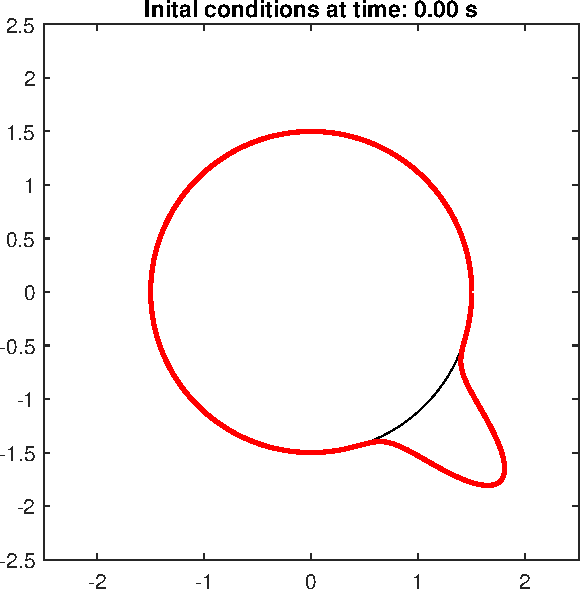
\includegraphics[width=0.4\textwidth]{C:/Users/Matteo/Shallow-Water-Equations/plots/SWE-spherical-1d-initial_conditions.pdf}
    \caption{Initial conditions for the 1D linearized shallow water equations in spherical coordinates.}\label{fig:swe_spherical_1d_initial_conditions}
\end{figure}




\section{The Riemann problem}
We will now define the Riemann problem, since it plays a crucial role in the finite volume method.
In the Riemann problem we distinguish between what we call a wet bed and a dry bed. 
A wet bed is the case where the water depth is positive everywhere, whereas a dry bed is the case where the water depth is zero in some cells.
The special Riemann problem where parts of the bed are dry is dealing with the so-called dry fronts or wet/dry fronts, which are challenging to handle numerically.
We will leave these cases for now, and only consider wet bed problems.
The Riemann problem for the shallow water equations in 1D with a zero source term is defined as the initial-value problem (IVP)~\cite{Toro2024}:
\begin{equation}\label{eq:Riemann_problem}
    \begin{aligned}
        \text{PDEs: } &\mathbf{U}_t + {\mathbf{F(U)}}_x = 0, \\
        \text{ICs: } &\mathbf{U}(x, 0) = \begin{cases}
            \mathbf{U_L}, & \text{if  } x < 0, \\
            \mathbf{U_R}, & \text{if  } x > 0.
        \end{cases}
    \end{aligned}
    \end{equation}
The vectors $\mathbf{U}$ and $\mathbf{F(U)}$ in~\eqref{eq:Riemann_problem} are given by
\begin{align}
    \mathbf{U} = \begin{bmatrix}
        h \\ hu \\ hv
    \end{bmatrix}, \quad
    \mathbf{F(U)} = \begin{bmatrix}
        hu \\ hu^2 + \frac{1}{2}gh^2 \\ hvu
    \end{bmatrix},
\end{align}
and the initial conditions $\mathbf{U_L}$ and $\mathbf{U_R}$ are
\begin{align*}
    \mathbf{U_L} = \begin{bmatrix}
        h_L \\ h_L u_L \\ h_L v_L
    \end{bmatrix}, \quad 
    \mathbf{U_R} = \begin{bmatrix}
        h_R \\ h_R u_R \\ h_R v_R
    \end{bmatrix},
\end{align*}
which represents the conditions at time $t = 0$ s in the left and right states of $x = 0$ m.
The function $\mathbf{U}$ is piecewise constant, with a discontinuity at $x = 0$ m.
The Riemann problem can be solved either exactly or approximately.
However, in this project we will focus on approximate Riemann solvers, which are able to solve the Riemann problem with high accuracy and efficiency.
Various approximate Riemann solvers exist, based on finding an approximate solution to the Riemann problem.
Some of these solvers will be considered in the next section.
An interesting example of a Riemann problem is the so-called dam break problem, which is presented next.

\subsection{The Dam-Break problem}
We now introduce the dam-break problem, a scenario of significant physical interest.
This problem models the sudden release of water following the collapse of a dam, making it highly relevant for studying natural disasters such as floods and tsunamis.
As a classic test case for numerical methods, the dam-break problem is commonly used to test the ability of a method to capture discontinuities in the solution.
The dam-break problem is a special case of the Riemann problem~\eqref{eq:Riemann_problem}.
The difference is that in the dam-break problem, the initial velocity components, $u_L, u_R, v_L$ and $v_R$, are zero, whereas in the Riemann problem they are allowed to be distinct from zero.
The initial setup is visualized in \autoref{fig:dam-break-problem}.
\begin{figure}[H]
    \centering
    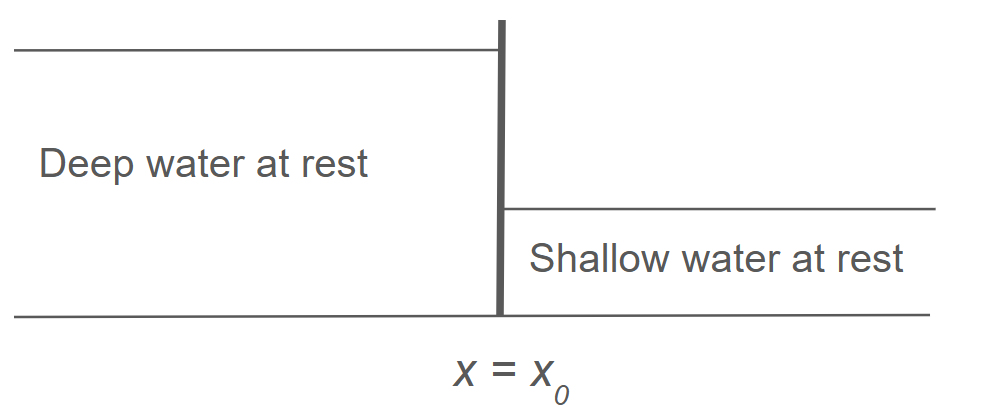
\includegraphics[width=0.5\textwidth]{C:/Users/Matteo/Shallow-Water-Equations/figs/dam-break-problem.png}
    \caption{Initial conditions for the dam-break problem. An infinitely thin wall at $x=x_0$ divides two sections of water with different water levels.}\label{fig:dam-break-problem}
\end{figure}
We can use the shallow water equations to model the flow of water in the dam-break problem, approximately, if we assume that the wall collapses instantaneously at $t=0$ s.
In this project we solve both the dam-break problem and cases of the Riemann problem, where the inital fluid velocity is nonzero.
The results are presented in \autoref{ch:numerical_results}.

\subsection{Solving the Riemann problem exactly by wave decomposition}
To get a better understanding of the flow in shallow water, we provide some very short background information about the wave structures in the solution of the Riemann problem.
In general, the wave structure in the solution of the Riemann problem~\eqref{eq:Riemann_problem} consists of three wave families separating four regions.
The wave families are denoted $W_1, W_2, W_3$ and the regions are the spaces between the wave families, denoted by $R_0, R_1, R_2$ and $R_3$.
The wave structure is illustrated in \autoref{fig:riemann_sol_general}.
\begin{figure}[H]
    \centering
    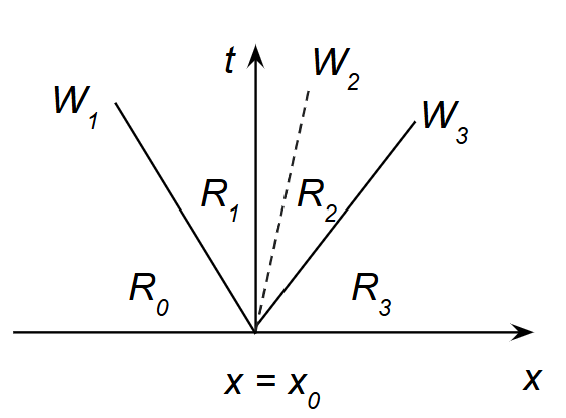
\includegraphics[width=0.5\textwidth]{C:/Users/Matteo/Shallow-Water-Equations/figs/riemann_sol_general.png}
    \caption{General wave structure in the solution of the Riemann problem.}\label{fig:riemann_sol_general}
\end{figure}
From \autoref{fig:riemann_sol_general} we see how the solution consists of three waves.
The left and right waves are either shock waves or rarefaction waves, and correspond to the one-dimensional shallow water equations.
The middle wave arises from the $y-$momentum equation in~\eqref{eq:Riemann_problem} and is always a shear wave.
The region between the left and right wave is called the star region and is interesting, since we do not know the solution in this region.
The star region is divided into two subregions $R_1$ and $R_2$.
The states in the regions are (from left to right) $U_L, U_{*L}, U_{*R}$ and $U_R$, where $U_L$ and $U_R$ are known, as these are the initial conditions.
The states $U_{*L}$ and $U_{*R}$ are in the regions $R_1$ and $R_2$, i.e., the star region and are unknown.
In the star region, we use $h_*$ to denote the water depth and $u_*$ to denote the velocity.
We can use $h_*$ to determine whether the left and right waves are shock waves or rarefaction waves.
Since we are considering the wet bed case, we can use the following characteristic:
\begin{equation*}
    \begin{cases}
        \text{The left wave is a shock wave} & \text{if } h_* > h_L, \\
        \text{The left wave is a rarefaction wave} & \text{if } h_* \leq h_L, \\        
    \end{cases} 
\end{equation*}
and similarly for the right wave:
\begin{equation*}
    \begin{cases}
        \text{The right wave is a shock wave} & \text{if } h_* > h_R, \\
        \text{The right wave is a rarefaction wave} & \text{if } h_* \leq h_R. \\        
    \end{cases} 
\end{equation*}
A shock wave is characterized by a discontinuity in the solution.
On each side of the shock wave, the water properties, such as height and velocity, differ significantly.
In contrast, a rarefaction wave represents a smooth transition in the solution.
The water height and velocity change gradually across the wave, and the properties are more similar on each side of the wave, without the sharp edges seen in a shock wave.
In the solution of the Riemann problem~\eqref{eq:Riemann_problem} there are four possible wave patterns outcomes, which are combinations of shock waves and rarefaction waves.
The left and right waves are either shock waves or rarefaction waves.
The four possible wave patterns are as follows:
\begin{enumerate}[label= (\alph*)]
    \item Left rarefaction, right shock,
    \item Left shock, right rarefaction,
    \item Both left and right rarefaction,
    \item Both left and right shock.
\end{enumerate}
In the example of the dam-break problem, with inital conditions as in Figure~\ref{fig:dam-break-problem}, the solution consists of a left rarefaction wave and a right shock wave.
This means that the shock wave moves to the right and is characterized by a discontinuity in the solution and a high speed.
Whereas, the rarefaction wave moves to the left and is characterized by a more smooth transition in the solution and a lower speed.
The Riemann solver computes the flux across the interface between two cells, considering the left and right states.
The numerical fluxes calculated by the Riemann solver allow for the determination of the state in the star region, which represents the solution at the interface between the two regions.
This is essential for determining whether the wave is a shock or a rarefaction wave, ensuring both the stability and accuracy of the numerical scheme.
In summary, Riemann solvers and numerical fluxes are crucial for solving for the states in the star region, which are then used to update the solution at each timestep.

%Hence the structure of the solution in general is shown in the figure below.
%From the figure we see that the solution consists of three waves, a left wave, a middle wave and a right wave, which together seperate four regions, described by the vector
%\begin{align*}
%\mathbf{W} = \begin{bmatrix}
%    h \\ hu \\ hv
%    \end{bmatrix}.
%\end{align*}
%The four regions are describes by $\mathbf{W}_L$ (left data), $\mathbf{W}_R$ (right data), $\mathbf{W}_{*L}$ and $\mathbf{W}_{*R}$, which both denote star region data.
%We are interested in the star region data, since these are the unknowns.
%Based on the given initial conditions, we must determine the types of waves.
%Second, it is known that across the left and right waves, both $h$ and $u$ change but $v$ remains constant.
%Whereas across the middle wave, $v$ changes but $h$ and $u$ remain constant.
%That is, $h$ and $u$ remain constant in the star region.
%Thus the water depth and particle velocity are constant in the star region and are denoted by $h_*$ and $u_*$, respectively.

%The exact Riemann solver is a method that solves the Riemann problem exactly, and it is based on the solution of the Riemann problem~\eqref{eq:Riemann_problem}.
%There exist exact Riemann solvers which are very efficient and leads to Gudonov methods, that are only slightly more expensive than those based on approximate Riemann solvers~\cite{Toro2001-Shock}.

%But for now, we will consider the case where the solution consists of a single non-trivial wave and all other waves are assumed to have zero strenght.
%This is enough to solve the Riemann problem as it is always possible to solve the Riemann problem by considering one wave at a time.
%We denote the constant values of the water depth and particle velocity in the star region by $h_*$ and $u_*$, respectively.


\section{Numerical fluxes}
In this section we will study the numerical fluxes used to solve the SWE.
At each cell interface, we need to solve the Riemann problem~\eqref{eq:Riemann_problem} to find the numerical flux.
There are several numerical fluxes that can be used to solve the local Riemann problem, and we will consider some of them in this section.
The fluxes we consider are the Godunov method with an exact Riemann solver, the HLL, HLLC, Rusanov, Lax-Friedrichs, Lax-Wendroff and FORCE fluxes.
They are later implemented and tested in the numerical experiments in \autoref{ch:numerical_results}.

\subsection*{Godunov method with exact Riemann solver}
%\addcontentsline{toc}{subsection}{Godunov method with exact Riemann solver}
We consider the Godunov upwind method, which is a first-order accurate metod to solve non-linear systems of hyperbolic conservation laws~\cite{Toro2024}.
In the method we solve the non-linear Riemann problem at each cell interface.
The Godunov flux is given by
\begin{align*}
    \mathbf{F}_{i + \frac{1}{2}} = \mathbf{F}(\mathbf{U}_{i + \frac{1}{2}}),
\end{align*}
meaning that we solve the Riemann problem exactly to find $h^*$ and $u^*$, and then use these values to compute the flux as 
\begin{align*}
    \mathbf{F}_{i + \frac{1}{2}} = \begin{bmatrix}
        h^* u^* \\ h^* {(u^{*})}^2 + \frac{1}{2} g {(h^{*})}^2
    \end{bmatrix}.
\end{align*}

\subsection*{HLL}
%\addcontentsline{toc}{subsection}{HLL}
The HLL (Harten, Lax and van Leer) approach assumes a two-wave structure of the Riemann problem.
The solver is based on the data $\mathbf{U}_L := \mathbf{U}_i^n, \mathbf{U}_R := \mathbf{U}_{i+1}^n$ and fluxes $\mathbf{F}_L := \mathbf{F}(\mathbf{U}_L), \mathbf{F}_R := \mathbf{F}(\mathbf{U}_R)$.
The HLL flux is given by
\begin{align}\label{eq:HLL_flux}
    \mathbf{F}_{i + \frac{1}{2}} = \begin{cases}
        \mathbf{F}_L & \text{if } S_L \geq 0, \\
        \mathbf{F}^{HLL} \equiv \frac{S_R \mathbf{F}_L - S_L \mathbf{F}_R + S_L S_R (\mathbf{U}_R - \mathbf{U}_L)}{S_R - S_L} & \text{if } S_L \leq 0 \leq S_R, \\
        \mathbf{F}_R & \text{if } S_R \leq 0.
    \end{cases}
\end{align}
The wave speeds $S_L$ and $S_R$ must be estimated in some way, and one possibility is to use 
\begin{align*}
    S_L = u_L - a_L q_L, \quad S_R = u_R + a_R q_R,
\end{align*}
where $a_L = \sqrt{g h_L}, a_R = \sqrt{g h_R}$ and  $q_K (K=L, R)$ is given by 
\begin{align*}
    q_K = 
    \begin{cases}
        \sqrt{\frac{1}{2}\left( \frac{(\hat{h} + h_K) \hat{h}}{h_K^2} \right) } & \text{if } \hat{h} > h_K, \\
        1 & \text{if } \hat{h} \leq h_K.
    \end{cases}
\end{align*}
Here $\hat{h}$ is an estimate for the water depth in the star region, $h_*$.
In the two-rarefaction Riemann solver, the water depth $h$ in the star region is given by
\begin{align}\label{eq:two_rarefaction_hstar}
    h_* = \frac{1}{g} {\left( \frac{1}{2} (a_L + a_R) + \frac{1}{4} (u_L - u_R)  \right)}^2,
\end{align}
which is what we use in this project for $\hat{h}$ in the HLL solver.
Since this is a two-wave model, it is complete for one dimensional problems, but for the augmented system of equations in two dimensions, the HLL solver is not complete, as it ignores the middle wave, the shear wave.
This motivates the use of the HLLC solver, which is a modification of the HLL solver.

\subsection*{HLLC}
%\addcontentsline{toc}{subsection}{HLLC}
The HLLC (Harten, Lax, van Leer, Contact) solver is an extension of the HLL solver, which includes the middle wave, i.e., it is a three-wave model.
In addition to the wave speeds $S_L$ and $S_R$, the HLLC solver also requires the speed of the middle wave $S^*$.
We can write the HLLC numerical flux as
\begin{align*}
    \mathbf{F}_{i+\frac{1}{2}}^{HLLC} = \begin{cases}
        \mathbf{F}_L & \text{if } 0 \leq S_L, \\
        \mathbf{F}_{*L} & \text{if } S_L \leq 0 \leq S^*, \\
        \mathbf{F}_{*R} & \text{if } S^* \leq 0 \leq S_R, \\
        \mathbf{F}_R & \text{if } S_R \leq 0.
    \end{cases}
\end{align*}
The fluxes $\mathbf{F}_{*L}$ and $\mathbf{F}_{*R}$ are given by
\begin{align*}
    &\mathbf{F}_{*L} = \mathbf{F}_L + S_L (\mathbf{U}_L - \mathbf{U}_{*L}),\\
    &\mathbf{F}_{*R} = \mathbf{F}_R + S_R (\mathbf{U}_R - \mathbf{U}_{*R}),
\end{align*}
and the middle states $\mathbf{U}_{*L}$ and $\mathbf{U}_{*R}$ are given by
\begin{align*}
    U_{*K} = h_K \left( \frac{S_K - u_K}{S_K - S_*}  \right)
    \begin{bmatrix}
        1 \\ S_* \\ \psi_K
    \end{bmatrix}.
\end{align*}
The function $\psi_K$ can represent either a passive scalar $\psi(x,t)$ or the velocity component $v(x,t)$ if we consider the two-dimensional shallow water equations.
Mathematically $\psi(x,t)$ and $v(x,t)$ behave identically.
An estimate for the middle wave speed $S^*$ can be calculated as
\begin{align*}
    S^* = \frac{S_L h_R(u_R - S_R) - S_R h_L (u_L - S_L)}{h_R (u_R - S_R) - h_L (u_L - S_L)},
\end{align*}
where $S_L$ and $S_R$ are the wave speeds of the left and right waves, respectively.

\subsection*{Rusanov}
%\addcontentsline{toc}{subsection}{Rusanov}
The Rusanov flux uses the HLL framework, but with a different choice of wave speeds.
To obtain the flux, we assume that an estimate $S^+$ for the positive wave speed is available.
Then we set 
\begin{align}\label{eq:Rusanov_flux_part1}
    S_L = -S^+, \quad S_R = S^+.
\end{align}
By substituting~\eqref{eq:Rusanov_flux_part1} into the $\mathbf{F}^{HLL}$ in~\eqref{eq:HLL_flux}, we obtain the Rusanov flux as
\begin{align}\label{eq:Rusanov_flux}
    \mathbf{F}_{i+\frac{1}{2}}^{Rus} = \frac{1}{2} \left( \mathbf{F}_{L} + \mathbf{F}_{R}  \right)
    - \frac{1}{2} S^+ \left( \mathbf{U}_R - \mathbf{U}_L \right),
\end{align}
where a simple estimate for the wave speed $S^+$ is given by
\begin{align*}
    S^+ = \max ( |S_L|, |S_R|).
\end{align*}
There are some requirement for $S^+$ in~\eqref{eq:Rusanov_flux} to ensure stability.
It must hold that 
\begin{align*}
    S^+ \leq \frac{\Delta x}{\Delta t},
\end{align*}
where $\frac{\Delta x}{\Delta t}$ is called the mesh speed.
%This Rusanov sheme is upwind and based on a one-wave model.
%Therefore it is an incomplete Riemann solver.

\subsection*{Lax-Friedrichs}
%\addcontentsline{toc}{subsection}{Lax-Friedrichs}
In the Lax-Friedrichs method, we use the Rusanov flux, but with a different choice of wave speed.
That is, we set the wave speed $S^+$ as the largest possible speed, while still ensuring stability, i.e.,
\begin{align}\label{eq:Lax-Friedrichs_wave_speed}
    S^+ = \frac{\Delta x}{\Delta t}.
\end{align}
By inserting the wave speed~\eqref{eq:Lax-Friedrichs_wave_speed} into the Rusanov flux~\eqref{eq:Rusanov_flux}, we obtain the Lax-Friedrichs flux as
\begin{align*}
    \mathbf{F}_{i+\frac{1}{2}}^{LF} = \frac{1}{2} \left( {\mathbf{F}}_{L} + {\mathbf{F}}_{R} \right) - \frac{1}{2} \frac{\Delta x}{\Delta t} \left( \mathbf{U}_R - \mathbf{U}_L \right),
\end{align*}
where $\mathbf{F}_L = \mathbf{F}(\mathbf{U}_L)$ and $\mathbf{F}_R = \mathbf{F}(\mathbf{U}_R)$.
The Lax-Friedrichs method is a centred method, which is first-order accurate.

\subsection*{Lax-Wendroff}
%\addcontentsline{toc}{subsection}{Lax-Wendroff}
There are several versions of the Lax-Wendroff flux, but in this thesis we will use the following flux:
\begin{equation}
    \begin{aligned}
        \mathbf{U}_{i+ \frac{1}{2}}^{LW} &= \frac{1}{2} \left( \mathbf{U}_{L} + \mathbf{U}_{R}  \right) - \frac{1}{2} \frac{\Delta t}{\Delta x} \left( {\mathbf{F}}_{R} - {\mathbf{F}}_{L} \right), \\
        \mathbf{F}_{i+\frac{1}{2}}^{LW} &= {{}\mathbf{F}{(\mathbf{U})}_{i+ \frac{1}{2}}^{LW}}.
    \end{aligned}
\end{equation}
The Lax-Wendroff method is a centred method, which is second-order accurate in space and time.

\subsection*{FORCE}
%\addcontentsline{toc}{subsection}{FORCE}
The FORCE scheme (First-Order Centred) is a combination of Lax-Friedrichs and Lax-Wendroffs fluxes.
The numerical flux is given by
\begin{align*}
    \mathbf{F}_{i+ \frac{1}{2}}^{FO} = \frac{1}{2} \left( \mathbf{F}_{i+ \frac{1}{2}}^{LF} + \mathbf{F}_{i + \frac{1}{2}}^{LW}  \right),
\end{align*}
where $\mathbf{F}_{i+ \frac{1}{2}}^{LF}$ is the Lax-Friedrichs flux and $\mathbf{F}_{i+ \frac{1}{2}}^{LW}$ is the Lax-Wendroff flux.
The FORCE scheme is first-order accurate.
It is possible to extend the FORCE scheme to multiple dimensions on structured meshes by using dimensional splitting.

\chapter{Neural Networks and Fourier Neural Operators}\label{ch:FNO+NN}
So far, we have studied numerical methods for solving partial differential equations (PDEs).
The finite volume method (FVM), along with other numerical solvers such as the finite difference method (FDM) and finite element method (FEM), solves PDEs by discretizing the domain into a grid.
A finer grid improves the accuracy of the solution but also increases the computational cost, creating a trade-off between accuracy and efficiency.
Complex PDEs often require a fine grid to accurately capture the solution, which can be computationally expensive.

In this chapter, we introduce the use of data-driven methods for solving PDEs.
%The hope of these methods is that they are able to reduce computational costs while maintaining high accuracy by learning the underlying dynamics of the solution.
%The primary goal of these methods is to reduce computational costs while preserving high accuracy by learning the underlying dynamics of the solution.
We will introduce the concepts of convolutional neural networks (CNNs) and Fourier neural operators (FNOs).

\section{Convolutional Neural Networks}
Convolutional neural networks (CNNs) are a specialized class of artificial neural networks designed to process and analyze data with a grid-like topology, such as images or time-series data represented by 2D grids.
CNNs excel at extracting spatial featues from data through the use of convolutional layers, which apply learnable filters to detect patterns such as edges, shapes or textures.
These layers are typically followed by pooling layers for dimensionality reduction and fully connected layers for classification or regression tasks.
A key advantage of CNNs is their ability to reduce the number of parameters compared to fully connected networks by sharing weights across spatial regions, making them computationally efficient and less prone to overfitting when working with large inputs.
Although CNNs are traditionally used for image recognition tasks, their architecture is adaptable for time-series analysis, especially when the data is structured spatially or sequentially.

In this project, CNNs are used to solve the shallow water equations, by training on the solution data generated by the FVM solver.
We aim to learn the underlying dynamics of the system by training the CNN on sequences of input-output pairs, where the input is the state of the system at time $t$ and the output is the state at time $t + \Delta t$.
The network is trained to construct a flow map. % which predicts the state of the system at the next time step based on sequences of input data.
The flow map $\Phi^t: \mathbb{R}^n \rightarrow \mathbb{R}^n$ is defined such that, for all $x \in X$ and all $t \in \mathbb{R}$:
\begin{align*}
    \Phi^t(x_0) =  x(t),
\end{align*}
where $x(t)$ is the solution of the PDEs with initial condition $x(0) = x_0$.
The flow map satisfies
\begin{align*}
    \Phi(\Phi (x, t), s) = \Phi(x, s + t),
\end{align*}
A CNN can approximate the flow map $\Phi$ by training on data that pairs an initial state $x_0$ with its state at later times $x(t)$.
The goal is to learn the mapping:
\begin{align*}
    x(t) = \Phi_{CNN} (x_0), 
\end{align*}
where $\Phi_{CNN}$ is the CNNS' approximation of the flow map.
The CNN model is trained on input-output pairs of sequences of data, with a sequence length of $N$.
\begin{align*}
    \begin{bmatrix}
        x_0 \\ x_1 \\ \vdots \\ x_{N-1}
    \end{bmatrix}
    \to
    \begin{bmatrix}
        x_1 \\ x_2 \\ \vdots \\ x_{N}
    \end{bmatrix}
\end{align*}


Meaning the network takes sequences of input data, and predicts the corresponding output data.
The output of the CNN is the solution at the next time step, effectively learning the dynamics of the SWE through the time-series data.
This setup allows the model to capture both spatial and temporal dependencies in the data, leveraging the CNN's ability to learn localized featires while processing sequential information.
A pro of CNN's is that they are efficient. By processing data in parallel using convolutional layers, the CNN efficiently handles large datasets without requiring excessive computational resources.
Another pro is the adaptability. 
The model's ability to learn from sequential data makes it adaptable for time-series predictions in dynamic systems like the shallow water equations.
A con is the data representation. Representing time-series data as sequences may require preprocessing, which can introduce complexity or a potential loss of information.
There can also be temporal limitations, as CNNs lack explicit mechanisms to model long-term temporal dependencies (unless extended with additional architechtures like RNNs or Transformers).
We will test and evaluate the performance of the CNN model in \autoref{ch:data-driven-results}.

%A classical neural network (NN) learns a mapping from input to output, i.e., a mapping between finite-dimensional spaces.
%Convolutional Neural Networks (CNNs) are a type of neural network that is particularly well-suited for image processing tasks.
%CNNs are designed to recognize patterns in spatial data, such as images, by using convolutional layers.
%A convolutional layer applies a set of filters to the input data, which allows the network to learn spatial hierarchies of patterns.
%The filters are learned during the training process, enabling the network to automatically extract features from the input data.
%CNNs have been widely used in image classification, object detection, and image segmentation tasks, among others.

%While CNNs have shown promise for solving PDEs, they have limitations when it comes to capturing long-range dependencies in the data.
%PDEs often involve interactions between distant points in the domain, which can be challenging for CNNs to capture.
%Another issue we are facing in this project is non-linearities.
%Standard neural networks uses combinations of linear multiplications and non-linear activation functions to approximate non-linear functions.



\section{Fourier Neural Operators}
In this section, we introduce the concept of Fourier Neural Operators (FNOs), a method for approximating mappings between infinite-dimensional function spaces.
The theory and method described here are based on the paper~\cite{FNO_2021}.
The goal is to learn a mapping between two infinite dimensional spaces from a finite collection of input-output pairs. 
Consider the operator $G: A \to U$, which maps from an infinite-dimensional function space $A$ to another infinite-dimensional function space $U$.
We aim to approximate the exact operator $G$ by constructing the map
\begin{align*}
    G_{\theta}: A \mapsto U, \quad \theta \in \Theta,
\end{align*} 
where $\Theta$ is a finite-dimensional parameter space.
Consider the functions $a \in A$ and $u \in U$.
We assume access to data in the form of pointwise evaluations of these functions, i.e., we have access to the observations ${\{a_j, u_j \}}_{j=0}^N$, in a domain $D \subset \mathbb{R}^d$, which is bounded open set.
The first step is to create $v_0(x) = P(a(x))$ by the input layer $P$, which is typically a shallow fully-connected neural network.
The neural operator is iterative, meaning we apply several iterations of updates to obtain $v_1, v_2, \ldots$ up to $v_T$.
An update $v_t \mapsto v_{t+1}$ is defined as
\begin{align}
    v_{t+1}(x) := \sigma \left( W v_t(x) + \left( \mathcal{K}(a;\phi)v_t \right) (x) \right), \quad \forall x \in D,
\end{align}
where $W: \mathbb{R}^{d_v} \to \mathbb{R}^{d_v}$ is a linear transformation, and $\sigma: \mathbb{R} \to \mathbb{R}$ is a non-linear activation function.
The output $u(x) = Q(v_T(x))$ is the final update $v_T$ transformed by the output layer $Q$.
There are various types of operators, but the core of the Fourier neural operator lies in its kernel function $\mathcal{K}$.
We define the Fourier integral operator $\mathcal{K}$ as 
\begin{align}
    \left( \mathcal{K}(\phi)v_t \right) (x) := \mathcal{F}^{-1} \left( R_{\phi} \cdot (\mathcal{F}v_t ) \right)(x), \quad \forall x \in D,
\end{align}
where $\mathcal{F}$ is the Fourier transform, $\mathcal{F}^{-1}$ is the inverse Fourier transform, and $R$ is the linear transformation applied on the lower Fourier modes. 
By transforming the data into the Fourier domain, FNOs can take advantage of the periodicity and smoothness properties of the Fourier basis, which simplifies the learning process for functions defined over continuous domains.
This approach leverages the fact that differentiation with respect to time is equivalent to multiplication in the Fourier domain, distinct from the convolution theorem. CITE.
The network architechture for the FNO model is illustrated in \autoref{fig:fourier_neural_network}.
\begin{figure}[H]
    \centering
    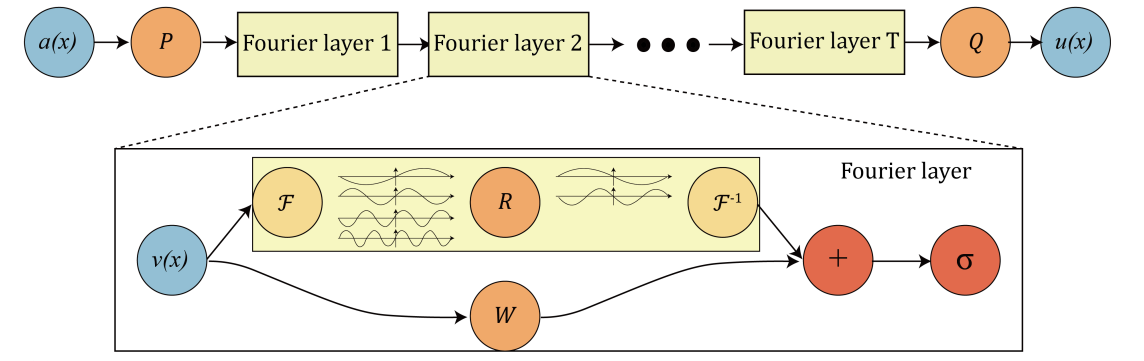
\includegraphics[width=0.7\textwidth]{C:/Users/Matteo/Shallow-Water-Equations/figs/fourier_neural_network.png}
    \caption{An overview of the network architecture with several Fourier layers. Illustration from~\cite{FNO_2021}.
            Top: Overall structure with input function $a$, input layer $P$, several Fourier layers, output layer $Q$ and output function $u$.\\
            Bottom: A Fourier layer consists of two parallel paths. Top is a Fourier transformation $\mathcal{F}$, a linear transformation $R$ and an inverse Fourier transformation $\mathcal{F}^{-1}$.
            The bottom path consists of a linear transformation $W$. The parts meet and undertake an activation function $\sigma$.}\label{fig:fourier_neural_network}
\end{figure}
From the top in \autoref{fig:fourier_neural_network} we see that the network consists of an input function $a(x)$, an input layer $P$, several Fourier layers, an output layer $Q$ and some output function $u(x)$.
As we only have access to pointwise evaluations of $a(x)$ and $u(x)$ these are what we will use. 
That is, our goal is to approximate the input-output mapping: 
\begin{align*}
    \begin{bmatrix}
        a_0 \\
        a_1 \\
        \vdots \\
        a_{N-1}
    \end{bmatrix}
    \to
    \begin{bmatrix}
        u_0 \\
        u_1 \\
        \vdots \\
        u_{N-1}
    \end{bmatrix}.
\end{align*}
In the context of this project we have that $a(x) = v_t(x)$ and $u(x) = v_{t+1}(x)$.

In the bottom of \autoref{fig:fourier_neural_network} we see the structure of a Fourier layer, which consists of two parallel paths.
In the top path, the data undergoes a Fourier transform $\mathcal{F}$, decomposing it into a sum of Fourier basis functions (sines and cosines) with varying frequencies, amplitudes and phases.
A linear transformation $R$ it the applied to filter out the higher Fourier modes, as illustrated in the figure, where high-frequency components are removed.
When implementing the model, we choose the number of Fourier modes to retain, depending on how much information we want to preserve.
Retaining more modes keeps more information, but may also introduce more noise and oscillations.
After filtering, the inverse Fourier transform $\mathcal{F}^{-1}$ is applied to reconstruct the data in its original form.
The bottom path involves a linear transformation $W$, and the two paths merge before applying a non-linear activation function $\sigma$.

A key advantage of FNOs is that since they learn mapping between function spaces, they are not constrained by a specific grid or mesh.
This allows them to transfor solutions across different grids, a process known as zero-show super-resolution.
The learned operator can generalize from the coarse grid to the fine grid without needing to be retrained, making it grid-independent.
This is a major advantage because it reduces the computational cost associated with fine-grid simulations.
In \autoref{ch:data-driven-results}, we will evaluate the performance of the implemented FNO model in this context, testing its ability to maintain high accuracy when making predictions on finer grids.

\subsection*{Multistep prediction}
We aim to develop a multi-step prediction model that can predict a specified number of time steps ahead.
The input-output pairs are given as $\{a_j, u_j\}_{j=0}^N$, where the points $\{u\}_{j=0}^N$ represent the values one time step after $\{a\}_{j=0}^N$.
We collect state pairs $\{v_t, v_{t+1}\}_{j=0}^N$ for training a flowmap.
Feeding this data into the model allows it to learn the flow map for the system.
We are dealing with time series data, and the original form of the FNO can predict one time step ahead.
However, for many applications, predicting multiple time steps ahead is more useful.
To enable multi-step predictions, we organize the input data into sequences.
The model is trained to predict the output state based on data from several previous time steps, with a specified sequence length.
That is, the input data is given as
\begin{align*}
    \{v_{t-n}, v_{t-n+1}, \dots, v_{t+1}\}_{j=0}^N,
\end{align*}
where $n$ is the sequence length.

We will conduct experiments to determine the optimal sequence length for our model.

During prediction, the model's output is added to the input as the newest data point, replacing the oldest data.
This process is repeated until predictions for the desired number of future time steps are made.
The process is illustrated in \autoref{fig:multistep_pred_flowchart}.
\begin{figure}[H]
    \centering
    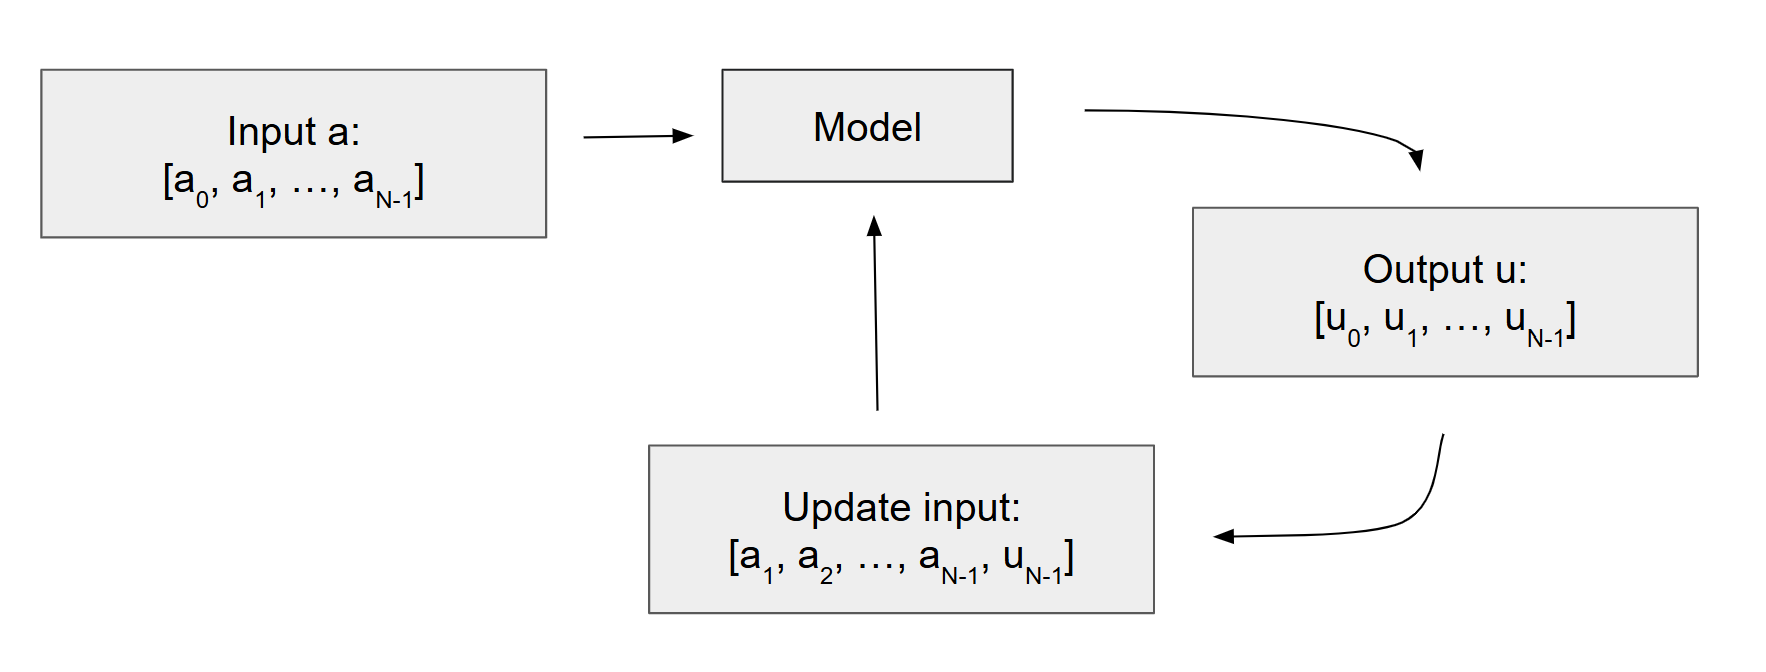
\includegraphics[width=0.7\textwidth]{C:/Users/Matteo/Shallow-Water-Equations/figs/multistep_pred_flowchart.png}
    \caption{Flowchart of the multi-step prediction process.}\label{fig:multistep_pred_flowchart}
\end{figure}
The results of the multi-step prediction model will be presented in \autoref{ch:data-driven-results}.



%Another issue we are facing in this project is non-linearities.
%Whereas, neural operators approximate non-linear operators, by combining linear functions and non-linear activation functions with global integral operators. 

%Both methods require only data, not the PDE itself, which is a significant advantage when the governing PDE is unknown.


\newpage
\chapter{Data generation}\label{ch:method}
In this chapter, we outline the process of generating the data required for the data-driven methods.
This step is critical, as the quality and relevance of the data directly impact the training and performance of the models.
We begin by detailing the data generation process for the 1D SWE using the exact Riemann solver.
Next, we describe the approach for generating data for the 1D SWE in spherical coordinates.
Finally, we present the methodology for data generation in the context of the 2D SWE.

%We will also present the mesh generation for the sphere, which is used to solve the SWE in spherical coordinates.

\section{Data generation using the FVM}\label{sec:data_generation_fvm}
In this section we clarify the data generation using our numerical solver based on the Finite Volume Method (FVM).
The FVM is used to solve the SWE in 1D, in 1D with spherical coordinates, and in 2D.
We specify the initial conditions, the domain, and the parameters used in the data generation process.

\subsection*{1D SWE with exact Riemann solver}
In this section, we present how the so-called true solution is found in the code by solving the Riemann problem exactly.
The true solution is found by solving the Riemann problem exact, with 200 cells, and distinguishing between the wetbed or drybed case, and also identifying the shock and rarefaction waves.
First we caculate the wave speeds for the left and right states, respectively, as
\begin{align*}
    c_L = \sqrt{g h_L}, \quad c_R = \sqrt{g h_R},
\end{align*}
which are used to determine the critical water height $h_{\text{crit}}$ as
\begin{align*}
    h_{\text{crit}} = (u_R - u_L) - 2(c_L + c_R).
\end{align*}
If either $h_L \leq 0$ or $h_R \leq 0$, we are in a drybed case.
If $h_{\text{crit}} \geq 0$ it means the water depth is somehow critical, and we are in a drybed case,
If none of the above conditions are met, we are in a wetbed case.
Summarized:
\begin{align*}
    \begin{cases}
        \text{Dry-bed case} & \text{if }  h_L \leq 0, \quad  h_R \leq 0 \text{ or } h_{\text{crit}} \geq 0, \\
        \text{Wet-bed case} & \text{otherwise}.
    \end{cases}
\end{align*}
For a dry bed case, we then identify where the dry is located, i.e., if the left side is dry, the right side is dry, or the middle is dry, and calculate the wave speeds accordingly.
For a wet bed case, we compute the characteristics $h_*$ and $u_*$ for the star region.
We then identify the shock and rarefaction waves, and calculate the wave speeds for the left and right states, respectively.
The process is illustrated in \autoref{fig:flowchart_true_solution}.
\begin{figure}[H]
    \centering
    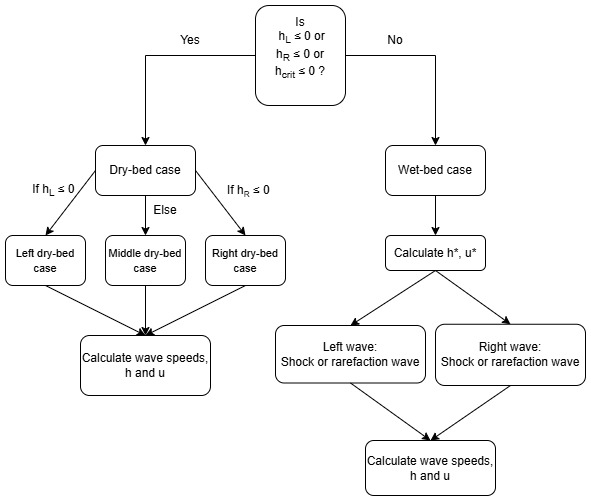
\includegraphics[width=0.8\textwidth]{C:/Users/Matteo/Shallow-Water-Equations/figs/flowchart_true_solution.jpg}
    \caption{Flowchart for generating the solution.}\label{fig:flowchart_true_solution}
\end{figure}
When generating the data, we need an initial condition for the water height $h$ and the velocity $u$.
In this study, we use the Gaussian function as the initial condition for the water height $h$, that is, we use the function
\begin{align}\label{eq:1D_swe_ic_gaussian}
    h(x,0) &= a \exp{\left(\frac{-{(x-\mu)}^2}{2\sigma^2}\right)},
\end{align}
where $a$ is the amplitude of the Gaussian, $\mu$ is the mean value, and $\sigma$ is the standard deviation.
We are working on the domain $x \in [0,1]$ and the parameters are set to $g = 9.81$ and $\sigma = 0.1$.
The value of $\mu$ is varied to generate different initial conditions, as seen in \autoref{fig:data_generation_initial}.
\begin{figure}[H]
    \centering
    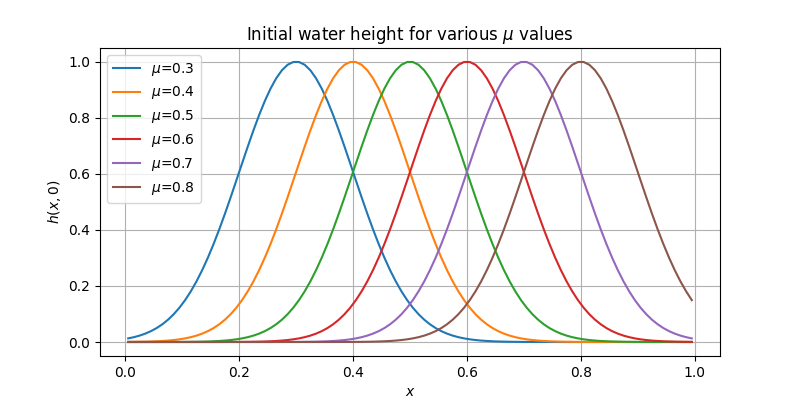
\includegraphics[width=0.8\textwidth]{C:/Users/Matteo/Shallow-Water-Equations/plots/data_generation_initial.png}
    \caption{Initial conditions for the data generation.}\label{fig:data_generation_initial}
\end{figure}
For the initial velocity $u$, we set it to zero, i.e., $u(x,0) = 0$. This means that the water is initially at rest.
The solver is validated by comparing the results with known test cases, such as the dam break problem.
We use a CFL number of $0.9$ and variable time steps.
We generate the data from $t = 0.0$ to $t_{\text{end}} = 1.0$.

\subsection*{Truncation error}
When generating data, it is essential to be aware of the truncation error.
Truncation error arises from the approximation of the solution of the differential equation by the numerical method.
Specifically, it is the difference between the exact solution and the numerical approximation.
The critical question is: after a certain number of time steps, how significant is this error?
If the error becomes too large, it raises concerms about the reliability of the generated data.
Excessive truncation error could compromise the accuracy of the model trained on this data.
Therefore, we must carefully evaluate and mitigate these risks to ensure the data's quality.
To assess the truncation error, we generate a more accurate solution using a finer grid.
This high-resolution solution serves as a reference for evaluating the numerical approximation.
By comparing the high-resolution solution with the numerical solution, we gain insights into the error introduces by the approximation.

In this study, we generate a reference solution for $N = 1000$ and compare it with the solution for $N = 100$ at the final time step, $t = 1.0$.
The results are shown in \autoref{fig:1D_SWE_truncation_error}.
\begin{figure}[H]
    \centering
    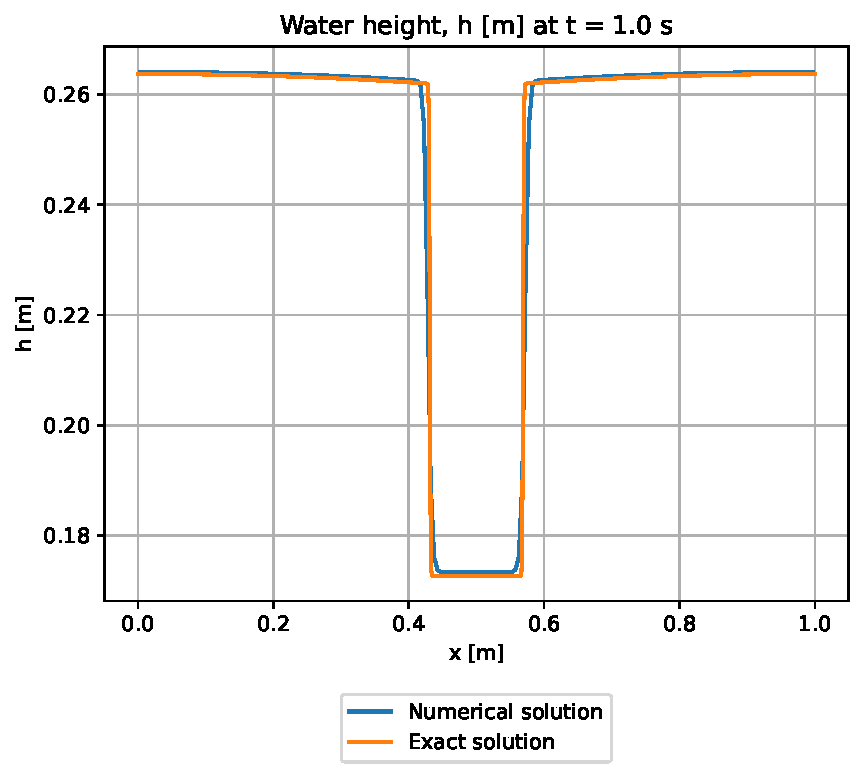
\includegraphics[width=0.5\textwidth]{C:/Users/Matteo/Shallow-Water-Equations/plots/truncation_error.pdf}
    \caption{Truncation error for the 1D SWE.}\label{fig:1D_SWE_truncation_error}
\end{figure}
From \autoref{fig:1D_SWE_truncation_error}, we observe that there is a small difference between the high-resolution solution and the numerical solution, as the high-resolution solution has a more discontinuous behavior.
However, overall the two solutions are almost identical, indicating that the truncation error is negligible.
This suggests that the data generated using the numerical solver is of high quality and can be used for training the data-driven models.

\subsection*{1D SWE in spherical coordinates}
We also consider the spherical shallow water equations in a 1D setting, focusing on the linearized SWE on a circular domain.
The length of the domain corresponds to the circumreference of the circle, $L = 2\pi$, and is discretized into $N = 500$ points.
The initial condition for the water height $h$ is specified as a Gaussian function wrapped around the circle, expressed as:
\begin{align}\label{eq:1D_swe_spherical_ic}
    h(\theta, 0) &= a \exp \left( \frac{-{(\theta-\mu)}^2}{2 \sigma^2} \right) ,\\
\end{align}
where the parameters are $a = 1$ and $\mu = \frac{\pi}{4}$.
We generate data for varying values of $\sigma$ to investigate the effect of the standard deviation on the model performance.
The data is generated for $\sigma = \frac{\pi}{8}, \sigma = \frac{\pi}{16}$ and $\sigma = \frac{\pi}{32}$.
The initial velocity $u$ is set to zero, i.e., $u(\theta,0) = 0$.
The time step size is fixed and set to $\Delta t = 0.0025$.
The initial conditions can be seen in \autoref{fig:swe_spherical_1d_initial_conditions_sigmas}.
\begin{figure}[H]
    \centering
    \begin{subfigure}[b]{0.3\textwidth}
        \centering
        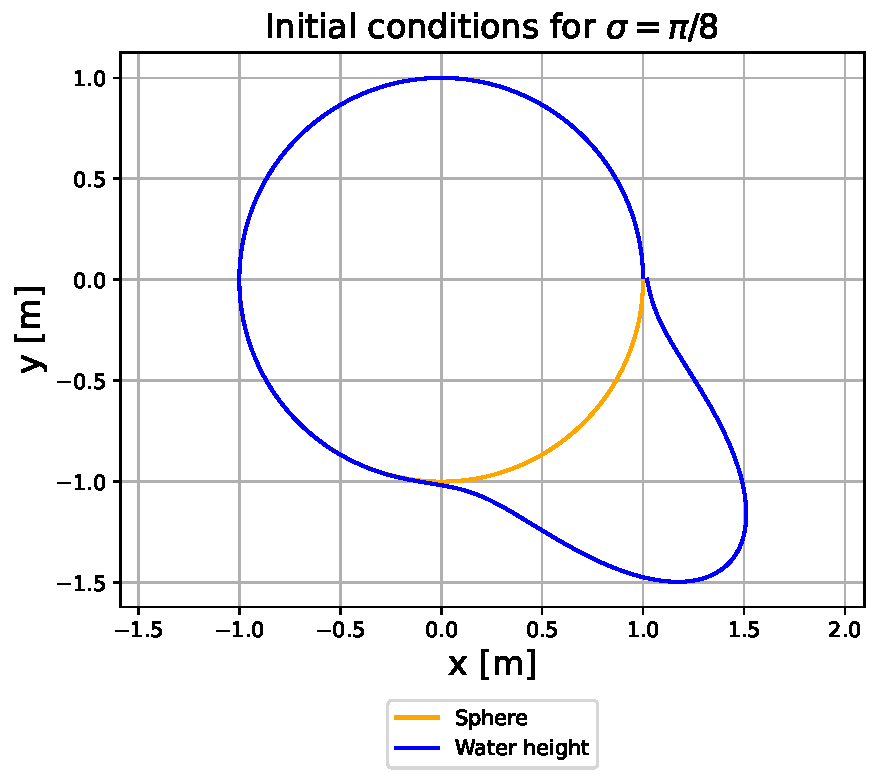
\includegraphics[width=\textwidth]{C:/Users/Matteo/Shallow-Water-Equations/plots/SWE-spherical-1d-initial_conditions_sigma1.pdf}
        \caption{$\sigma = \frac{\pi}{8}$.}\label{fig:swe_spherical_1d_sigma1}
    \end{subfigure}
    \hfill
    \begin{subfigure}[b]{0.3\textwidth}
        \centering
        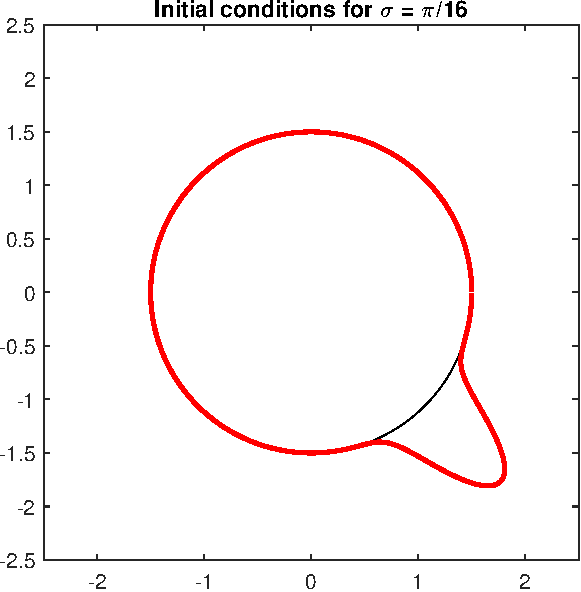
\includegraphics[width=\textwidth]{C:/Users/Matteo/Shallow-Water-Equations/plots/SWE-spherical-1d-initial_conditions_sigma2.pdf}
        \caption{$\sigma = \frac{\pi}{16}$.}\label{fig:swe_spherical_1d_sigma2}
    \end{subfigure}
    \hfill
    \begin{subfigure}[b]{0.3\textwidth}
        \centering
        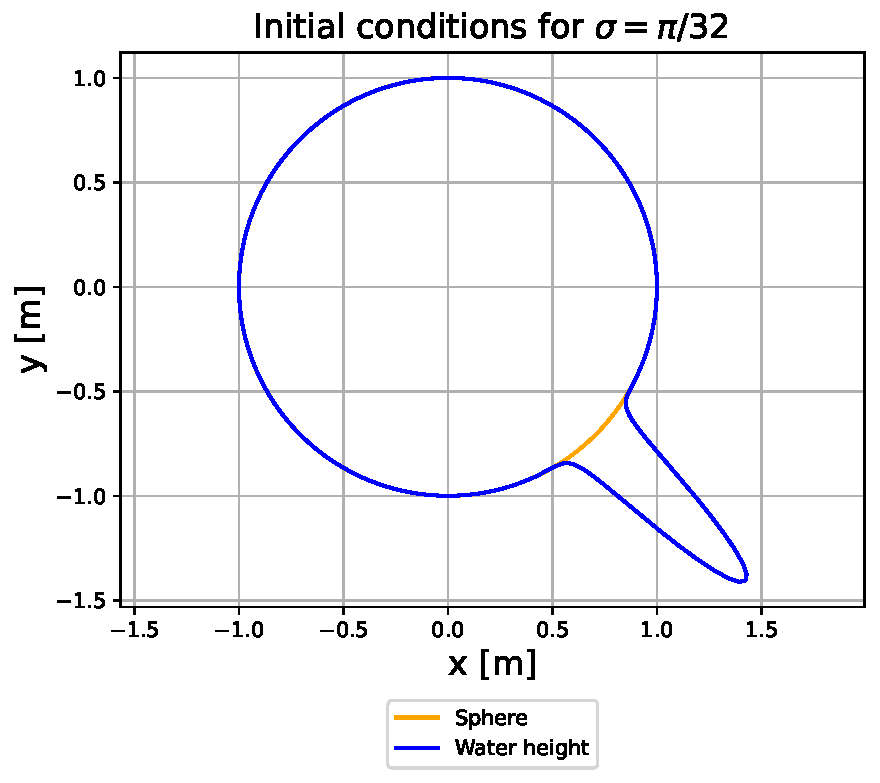
\includegraphics[width=\textwidth]{C:/Users/Matteo/Shallow-Water-Equations/plots/SWE-spherical-1d-initial_conditions_sigma3.pdf}
        \caption{$\sigma = \frac{\pi}{32}$.}\label{fig:swe_spherical_1d_sigma3}
    \end{subfigure}
    \caption{Initial conditions for the 1D linearized shallow water equations in spherical coordinates for different \(\sigma\) values.}\label{fig:swe_spherical_1d_initial_conditions_sigmas}
\end{figure}
From \autoref{fig:swe_spherical_1d_initial_conditions_sigmas}, we observe that the standard deviation \(\sigma\) affects the width of the Gaussian function.
The smaller the $\sigma$, the narrower the Gaussian function, meaning the curves are steeper.
This is to test the different models abilities to handle steep gradients.
The data is generated from $t = 0.0$ to $t_{\text{end}} = 1.0$.

\subsection*{2D SWE}
%For the 2D SWE, we also use Gaussian functions with parametric extension~\cite{Gaussian} to generate the initial conditions.
For the 2D SWE, we also use the Gaussian function as initial condition for the water height $h$, but now in two dimensions:
\begin{align*}
    h(x,y,0) &= h_0 + a \cdot \exp \left( -\frac{{(x-x_c)}^2 + {(y-y_c)}^2}{2\sigma^2} \right), 
\end{align*}
where $h_0$ is the initial water height outside of the Gaussian, $a$ is the amplitude of the Gaussian, $(x_c, y_c)$ is the center of the Gaussian, and $\sigma$ is the standard deviation.
The domain is $x,y \in [0,40]$ m and is discretized into $N$ points in each direction.
We use the parameters $h_0 = 1$, $a = 2$, $(x_c, y_c) = (20, 20)$, and $\sigma = 2$.
The initial velocity $u$ is set to zero, i.e., $u(x,y,0) = 0$.
The data is generated for different values of $N$ to investigate the effect of the grid resolution on the model performance.
To generate data like this also makes it possible to test the models abilities to transfer solutions to different grid resolutions.
The values of $N$ are $N = 64, N = 128$, and $N = 256$.
The time step size is variable and is set to satisfy the CFL condition, where the CFL number is set to $0.9$.
The initial conditions can be seen in \autoref{fig:2D_gauss_initial_condition}.
\begin{figure}[H]
    \centering
    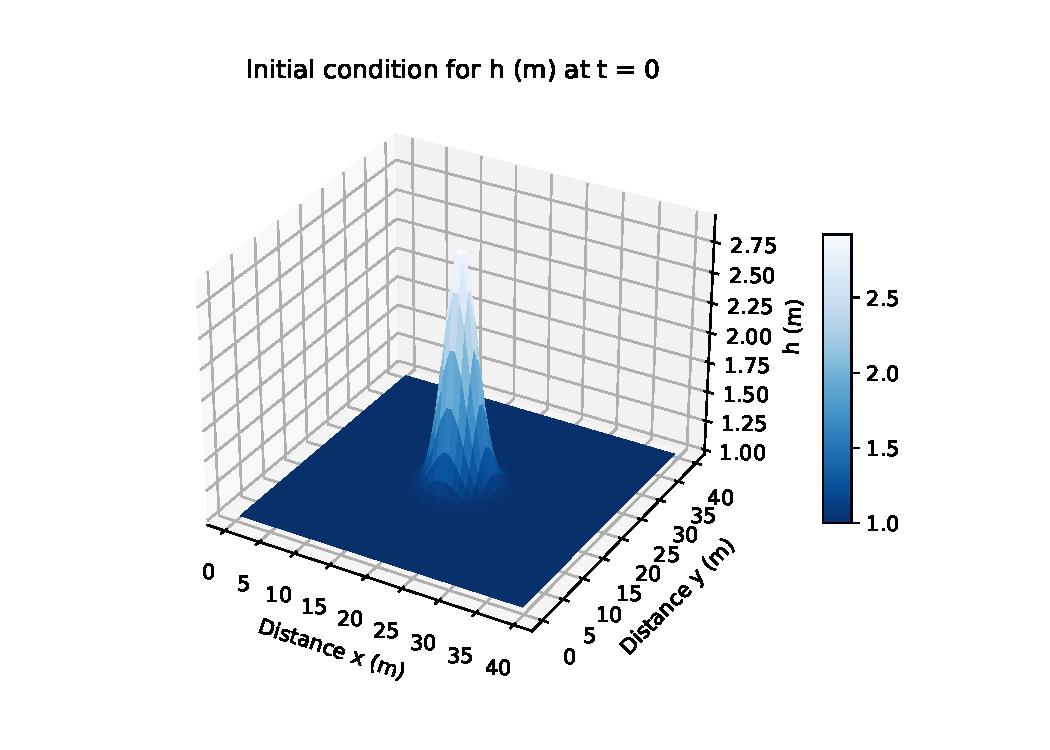
\includegraphics[width=0.8\textwidth]{C:/Users/Matteo/Shallow-Water-Equations/plots/2D_gauss_initial_condition.pdf}
    \caption{Initial condition for the 2D problem.}\label{fig:2D_gauss_initial_condition}
\end{figure}
To generate the data we use our FVM solver to solve the 2D SWE with the initial conditions given above, which is validated by comparing the results with known test cases.
The data is generated from $t = 0.0$ to $t_{\text{end}} = 10.0$.
In most of our test cases the models are using the data from $t = 0.0$ to $t_{\text{end}} = 5.0$, but we need the data to be generated for a longer time period to test the models ability to make long-term predictions.
Since we are making predictions beyond the data, the time step size is unknown, and we must work with a fixed time step size.
For generating data for long-term predictions, we employed a constant time step size of $\Delta t = 0.025$ s.
To ensure stability, the time step size must be sufficiently small.
To determine $\Delta t$, we analyzed the time step sizes used in the variable step data generation. 
By halving the smallest observed tme step size, we obtained $\Delta t = 0.025$ s.



\section{Data generation for the sphere}
A significant challenge in this project has been obtaining high-quality data for training data-driven methods on a sphere.
To tackle this, we are exploring various approaches for data generation, including the potential to create our own data and utilize external data sources.


\subsection*{Projecting 2D data to the sphere}
Our initial approach involved projecting the solution data from the 2D SWE onto the sphere.
To ensure stability and generate high-quality data, we set the CFL number to 0.8.
The coordinates $\theta$ (longitude) and $\phi$ (latitude) are treated similarly to $x$ and $y$ in the 2D case.
The grid is configured with $N_{\theta} = 200$ grid points in the $\theta-$direction and $N_{\phi} = 100$ grid points in the $\phi-$direction.
The higher resolution in the $\theta-$direction accounts for its double distance compared to the $\phi-$direction.
We use a Gaussian function as initial condition
\begin{align*}
    h(\theta, \phi, 0) = h_0 + a \cdot \exp\left( -\frac{{(\theta - \theta_c)}^2 + {(\phi - \phi_c)}^2}{{(2\sigma)}^2} \right),
\end{align*}
where $h_0 = 1$ m, $a = 3$, $\theta_c = \frac{3 \pi}{2}, \phi_c = \frac{\pi}{3}$, and $\sigma = \frac{\pi}{16}$.
The SWE are solved from $t = 0$ s to $t_{\text{end}} = 0.5$ s, using a variable step size $\Delta t$.
The simulation takes 199 time steps, resulting in an average time step size of $\Delta t \approx 0.0025$ s.
This value is significantly smaller than in the 2D case, likely due to the higher number of grid points, another domain and lower CFL number.
The results after some given time steps are presented in~\autoref{fig:sphere_projected_water_height_timesteps}.
\begin{figure}[H]
    \centering
    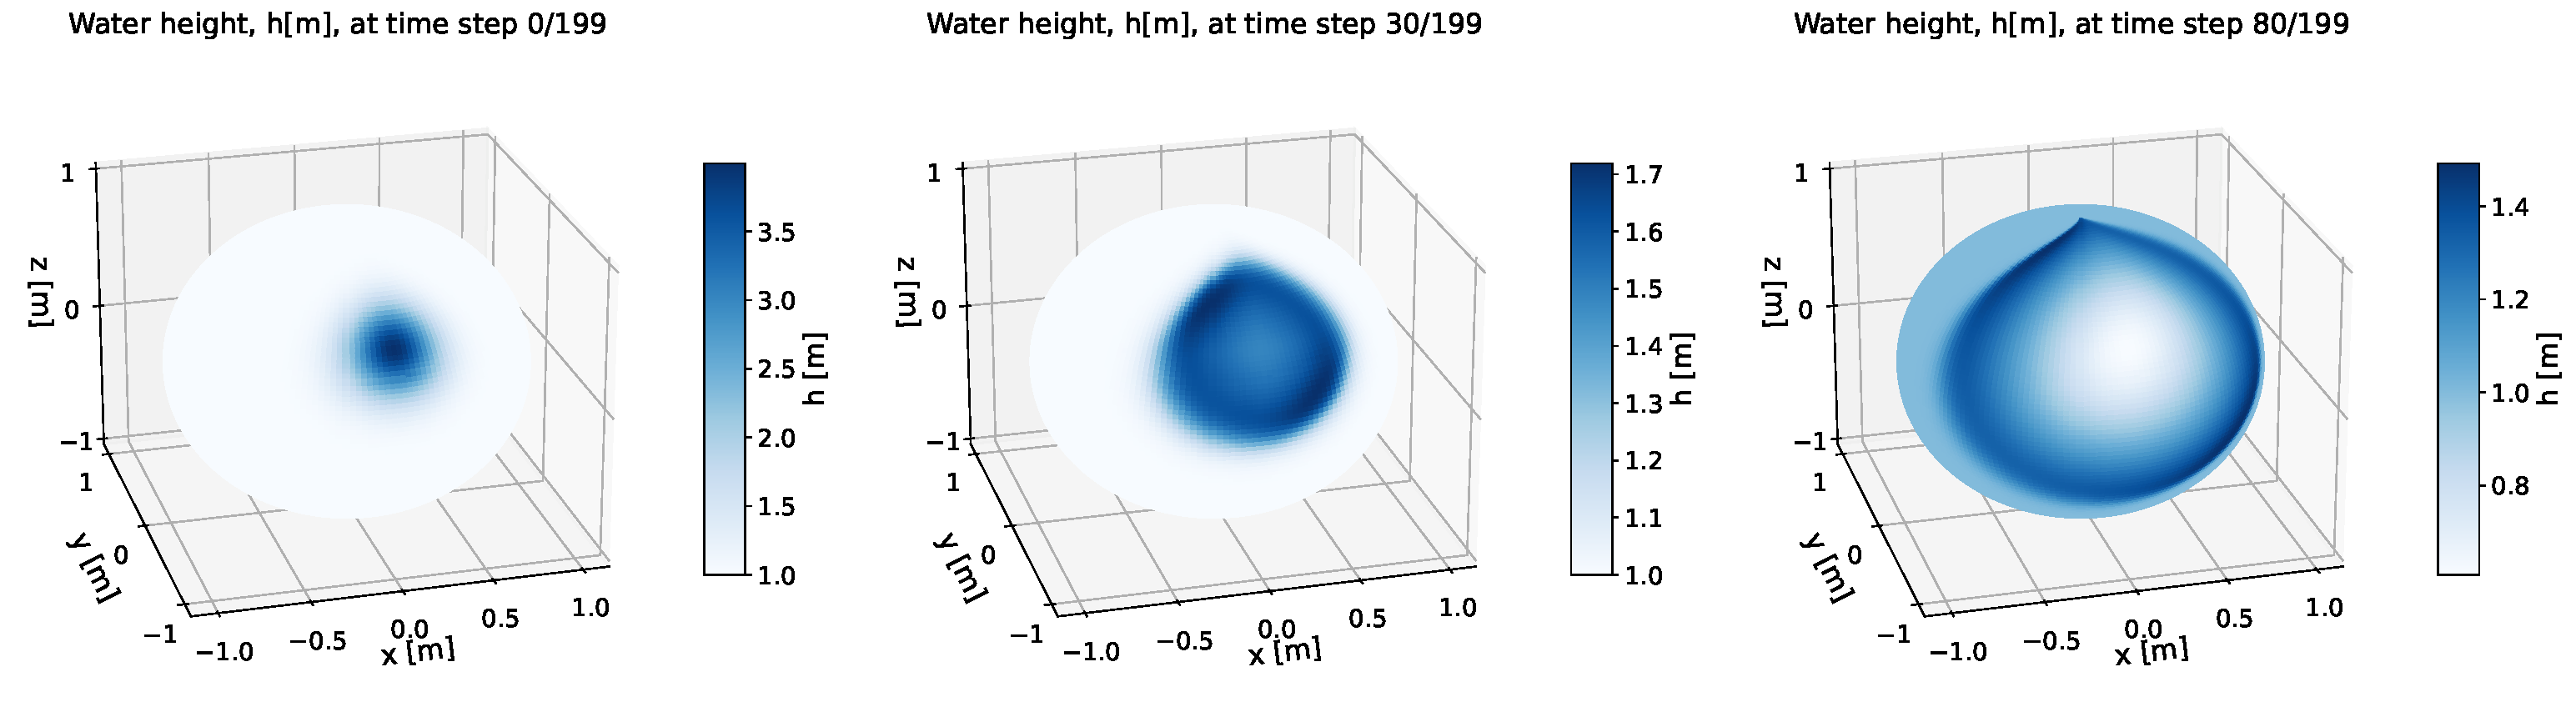
\includegraphics[width=0.95\textwidth]{C:/Users/Matteo/Shallow-Water-Equations/plots/sphere_projected_water_height_timesteps.pdf}
    \caption{Water height on the sphere for different timesteps.}\label{fig:sphere_projected_water_height_timesteps}
\end{figure}
In~\autoref{fig:sphere_projected_water_height_timesteps}we observe the evolution of the water height over time on the sphere.
The initial Gaussian bump propagates across the sphere, but singularities are present, especially at the poles.
These issues arise, amont other things, from neglecting the curvature of the sphere. 
While this approach might be acceptable for some applications, for instance when focusing on a small region near the equator, where the projection is more accurate, it is not suitable for our project.
Since our aim is to model the entire sphere, accounting for its curvature is essential.
Consequently, we cannot use this data.

\subsection*{Mesh generation for the sphere}
To solve the SWE on the sphere, we must use a different grid than the regular grid used in the 2D case.
One approach is to use an icosahedral grid, which approximates the sphere with triangles.
The grid structure allows for various levels of refinement, depending on the desired level of accuracy.
At each refinement level, the number of triangles increases by a factor of four, as each triangle is divided into four smaller triangles, meaning that the number of triangles increases drastically with each level of refinement.
The grid is generated using Matlab code from the Github repository~\cite{sphere_mesh_triangles} and then rewritten to Python.
The first four levels of refinement are shown in~\autoref{fig:icosahedral_grid}.
\begin{figure}[H]
    \centering
    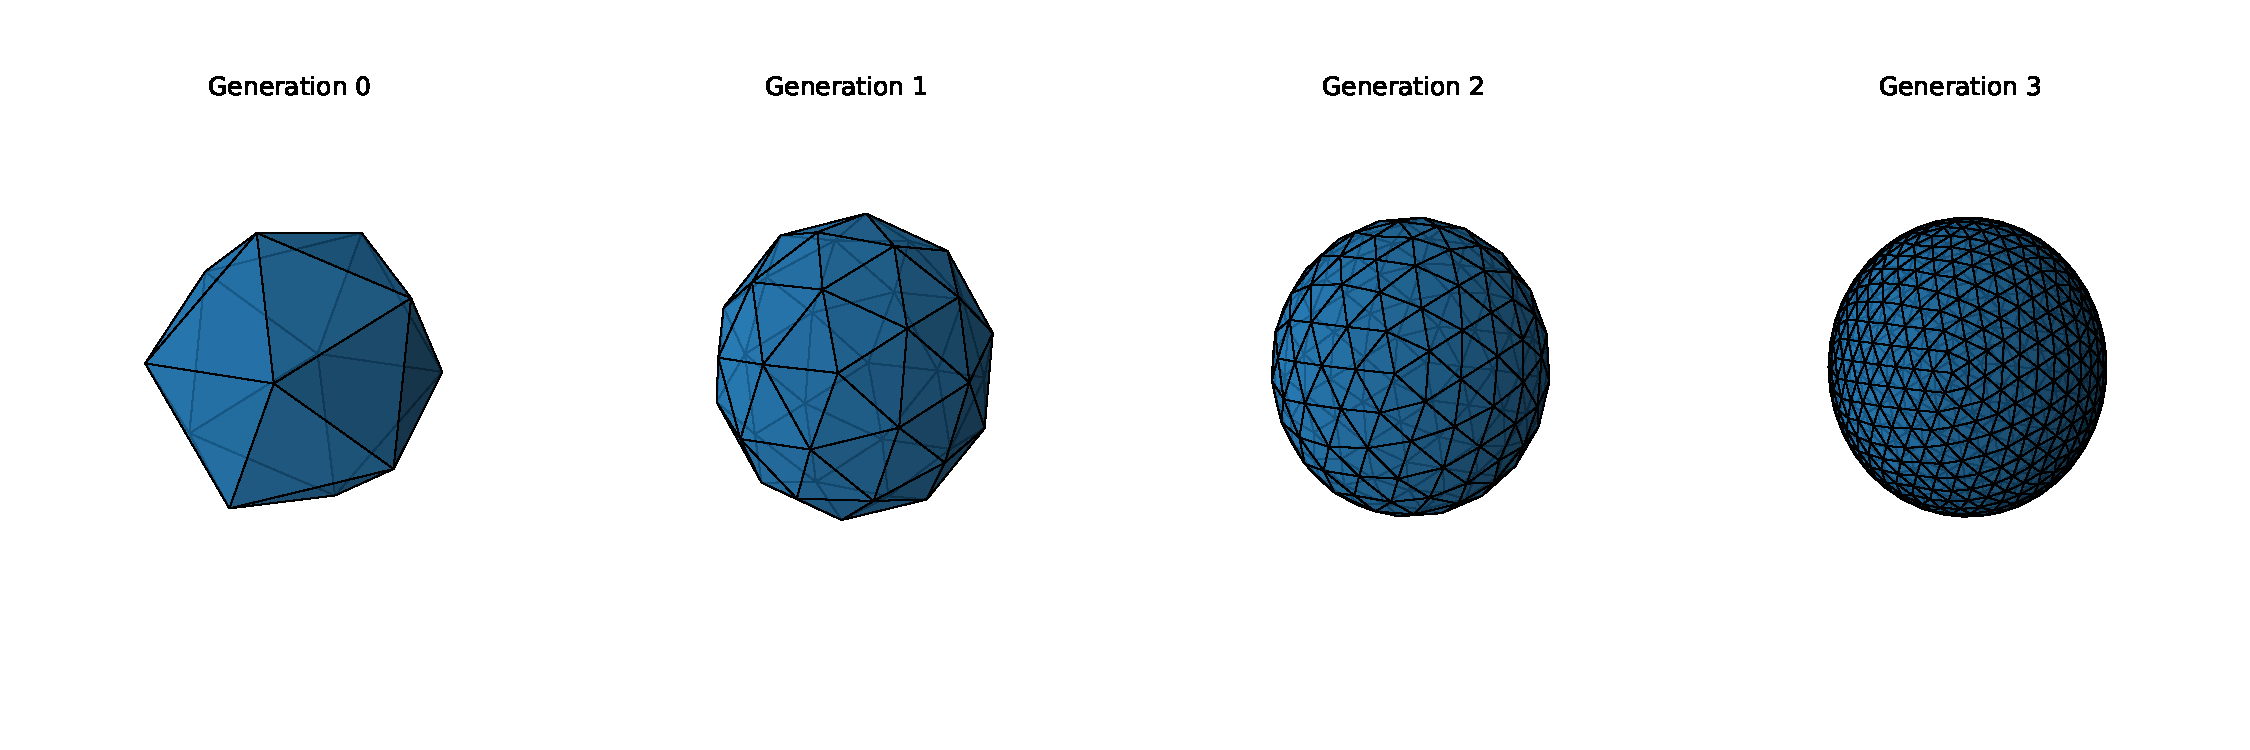
\includegraphics[width=\textwidth]{C:/Users/Matteo/Shallow-Water-Equations/plots/icosahedral_mesh_refinement.pdf}
    \caption{Icosahedral grid for the first 4 levels of refinement.}\label{fig:icosahedral_grid}
\end{figure}
In~\autoref{fig:icosahedral_grid} we see how the grid is refined at each level, resulting in a progressively more accurate representation of the sphere.
We will brieftly outline the process of solving the SWE on this grid structure, inspired by the finite element method (FEM).


We will shortly outline the process of solving the SWE on this grid structure, inspired by the finite element method (FEM).
The main idea is that for each triangle we keep track of which the neighboring triangles are. 
We also keep track of which interfaces the neighboring triangles share. 
This information is stored in various tables, known as the Element-to-Vertex, Element-to-Face, and Element-to-Element tables.
Each triangle is numbered, as well as each vertex.
The Element-to-Vertex (EToV) table stores the vertices of each triangle, meaning that each row corresponds to a triangle and the three columns correspond to the three vertices of the triangle.
The Element-to-Element (EToE) table can be made based on the EToV table.
The EToE table stores the neighboring triangles of each triangle, meaning that each row corresponds to a triangle and the three columns correspond to the three neighboring triangles, using the given labeling.
The Element-to-Face (EToF) table keeps track of which faces (edges) that are shared between two triangles, meaning for each triangle for each neighbor we must know which face the two triangles share.

The idea is then that for each interface we compute the fluxes between the triangles.
That is, we calcualte the fluxes the goes out of one triangle and into the neighbor.
This is to make sure the total flux overall is zero, meaning that the total volume of water is conserved.
However, we must be aware of the fact that the triangles are not on straigt lines, like the case in 2D. 
Meaning for each flux on each interface we must compute the contribution in the $\theta-$ and the $\phi-$direction.
Where previous we could more or less view the overall problem as two 1D problems, now they are interchanged.




\subsection*{External data sources}


\begin{figure}[H]
    \centering
    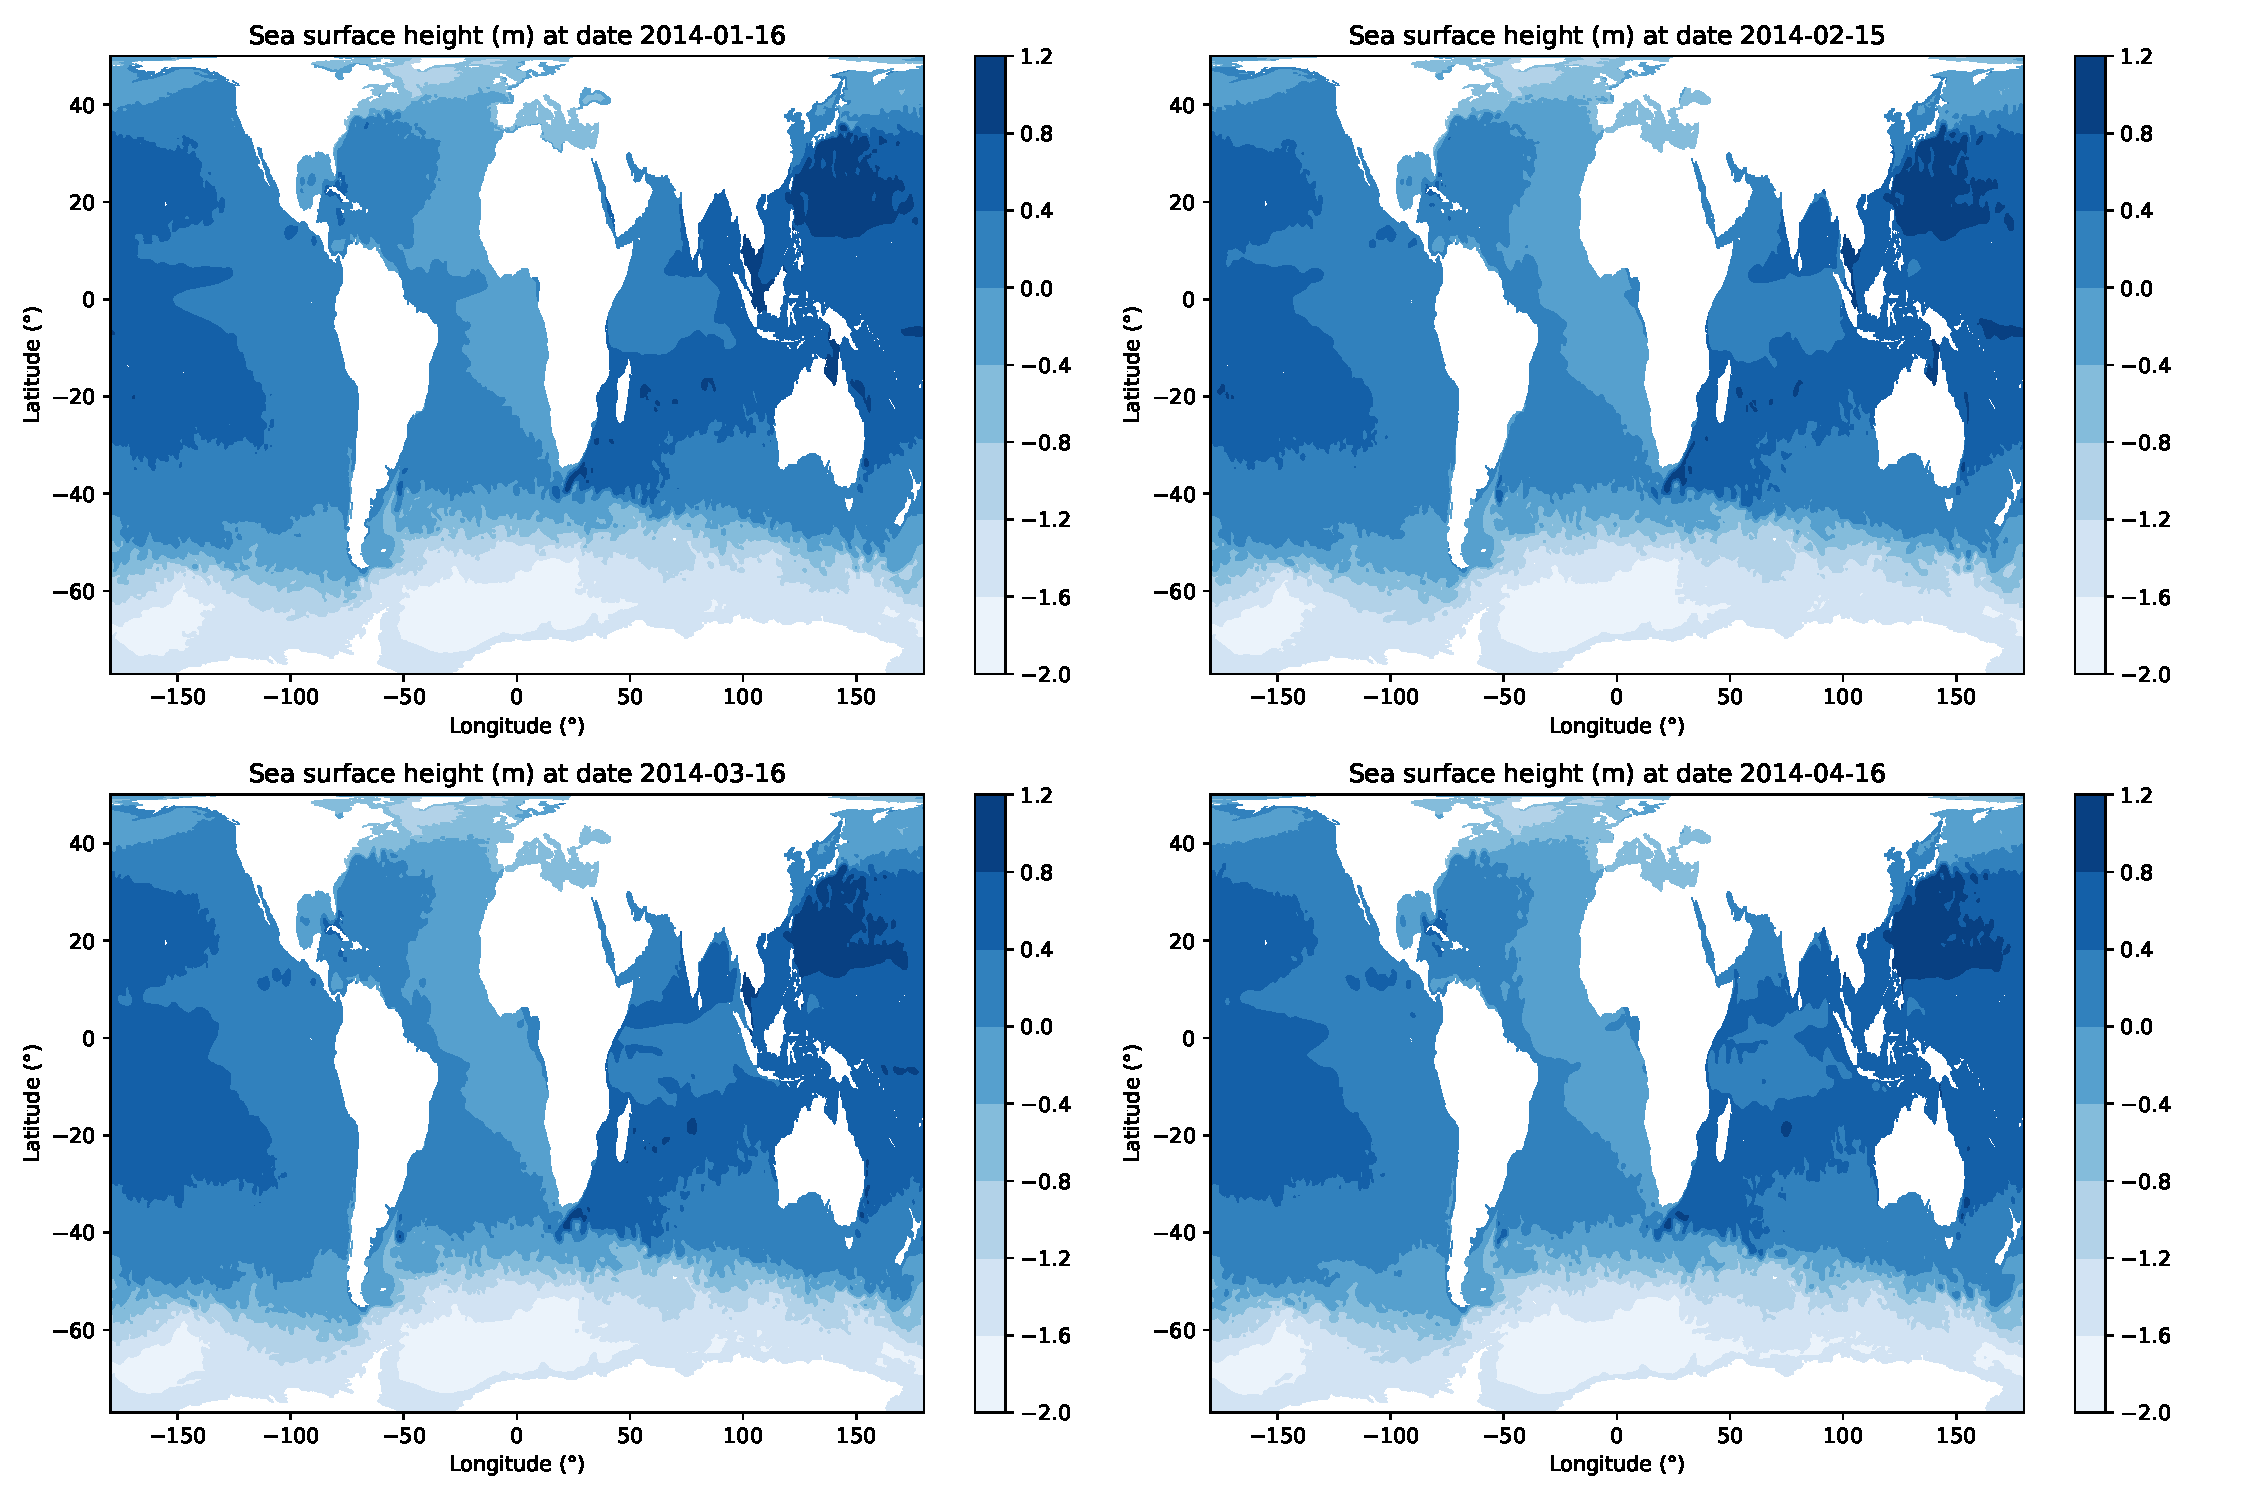
\includegraphics[width=0.95\textwidth]{C:/Users/Matteo/Shallow-Water-Equations/plots/ssh_field.pdf}
    \caption{Sea surface height as the diffference from reference sea surface height for the months Jan-Apr 2014.}\label{fig:copernices-ssh}
\end{figure}




\newpage
\input{chapters/05_Results.tex}
\section{Data-driven results}
In this section we present the results of the data-driven models.
We start by showing the numerical solution of the shallow water equations, then we present the predictions of the NN and FNO models.
Until now, we have mostly considered discountinuous initial conditions, but we will also consider smooth initial conditions in this section.
We solve the SWE with the following initial conditions:
\begin{equation}\label{eq:data-driven-initial-conditions-gauss}
    \begin{aligned}
        h(x, 0) &= h_0 \exp \left( \frac{-{(x-\mu)}^2}{2 \sigma^2} \right) ,\\
        u(x, 0) &= 0 , \\
    \end{aligned}
\end{equation}
where $h_0 = 1, \mu = 0.5, \sigma = 0.1$. 
The function $h(x, 0)$ is a Gaussian function, illustrated in Figure~\ref{fig:NN_initial_1D}.
\begin{figure}[H]
    \centering
    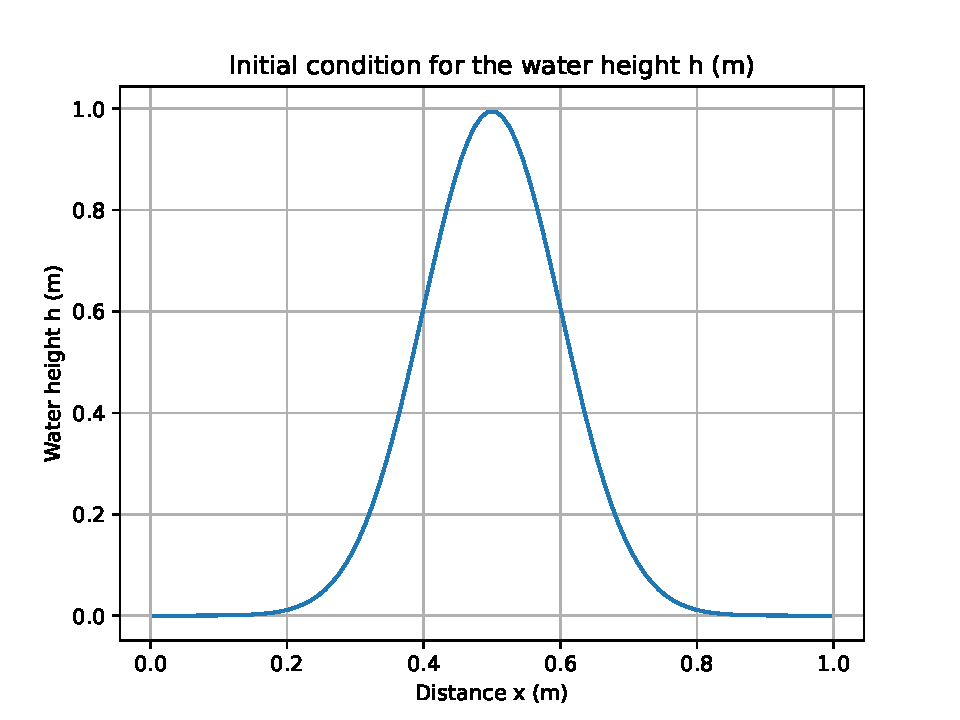
\includegraphics[width=0.5\textwidth]{C:/Users/Matteo/Shallow-Water-Equations/plots/NN_initial_1D.pdf}
    \caption{Initial conditions~\eqref{eq:data-driven-initial-conditions-gauss}.} \label{fig:NN_initial_1D}
\end{figure}
The domain is $ x \in [0, 1]$ with $N = 200$ points and the final time is $t = 1.0$.
We use a CFL number of $0.9$ and variable time steps.
The numerical solution is shown in Figure~\ref{fig:NN_initial}, in both a contour plot and a 3D plot.
\begin{figure}[H]
    \centering
    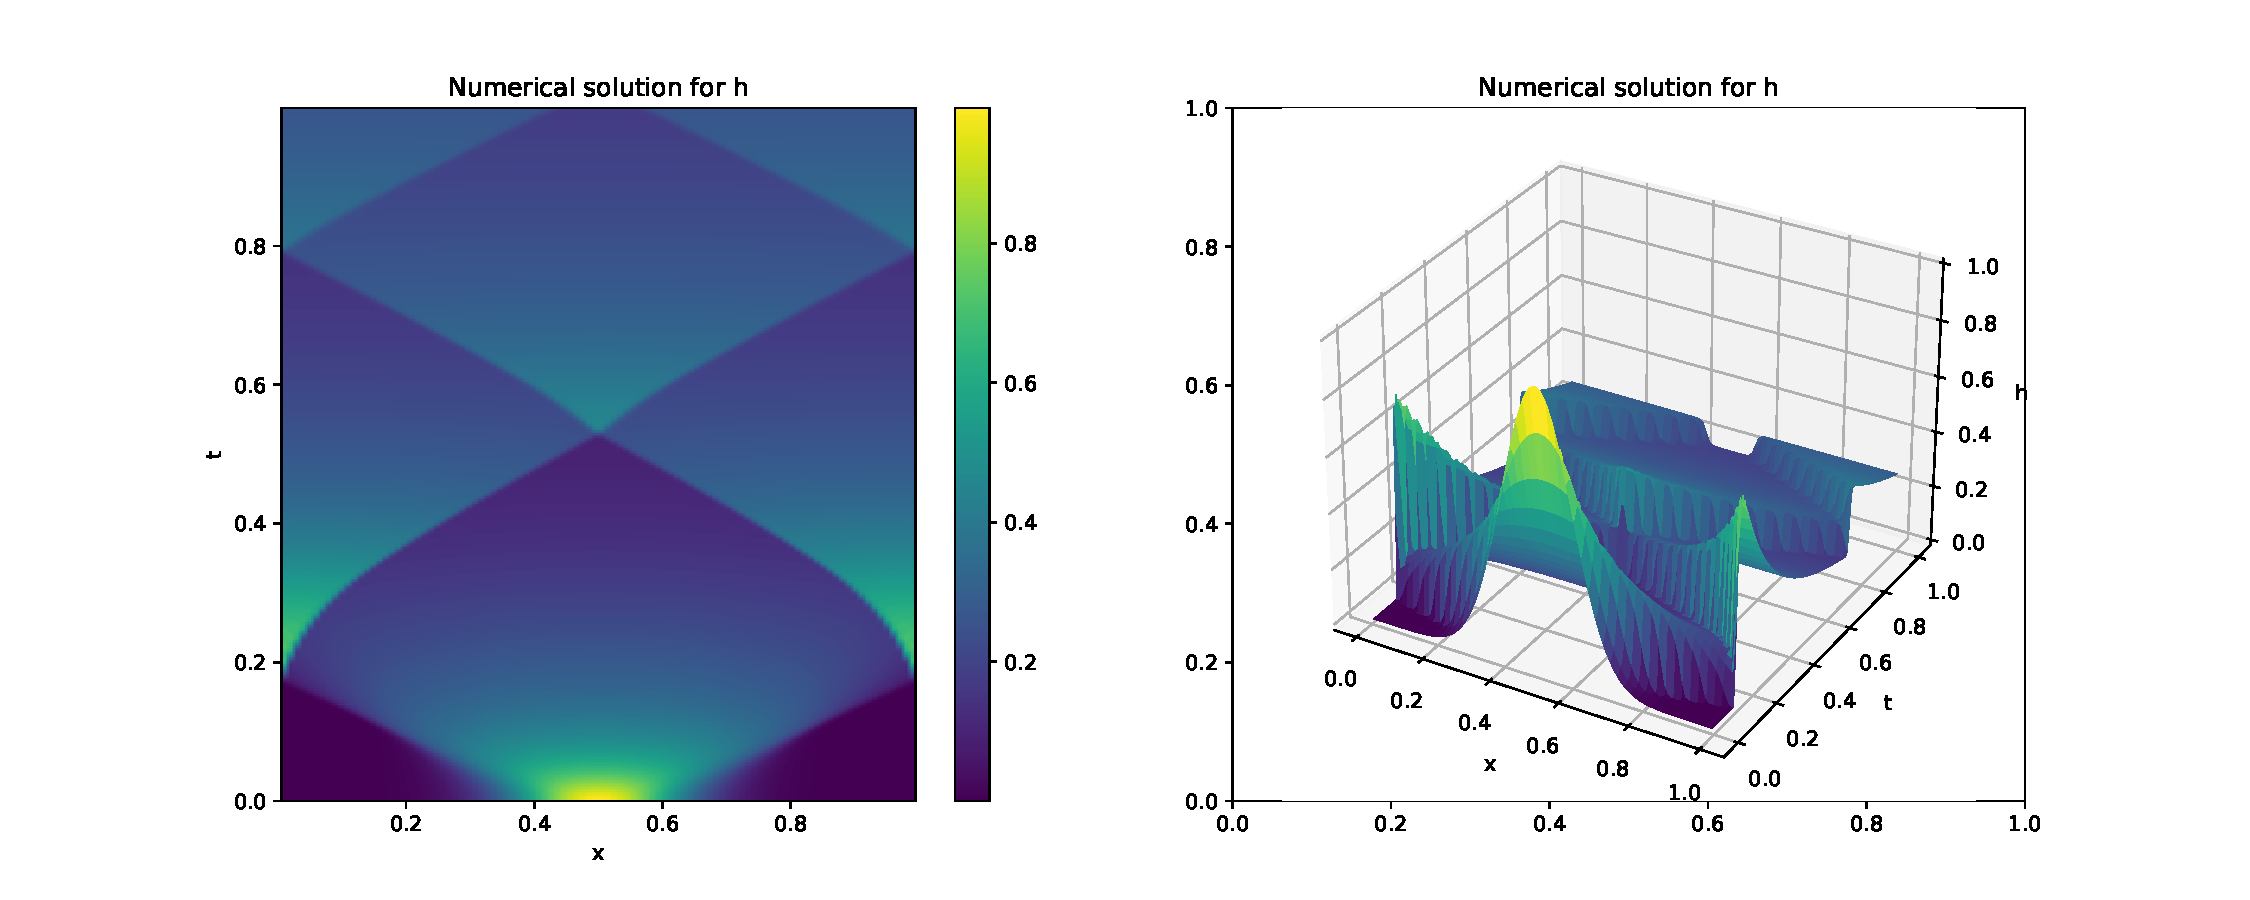
\includegraphics[width=0.7\textwidth]{C:/Users/Matteo/Shallow-Water-Equations/plots/NN_initial.pdf}
    \caption{Numerical solution of the shallow water equations with initial conditions~\eqref{eq:data-driven-initial-conditions-gauss}.}\label{fig:NN_initial}
\end{figure}


\subsection{RNN}
In the recurrent neural network, we train the model using the data generated by the numerical solution of the shallow water equations.
The model uses the data from the numerical solution to predict the solution at the next time step.
Meaning that the input and output data are the same, but shifted one time step.
This way, the model is supposed to learn the flowmap.
The RNN model consists of 4 layers.
%The neural network consists of the following layers: a input dense layer, three hidden dense layers with ReLU activation functions, a batch normalization layer for stability, a dropout layer to prevent overfitting, and an output dense layer.
The model has been trained using the Adam optimizer with a learning rate of $0.001$, a batch size of $32$ and a total of $500$ epochs.
We train the model on the data from $t = 0$ to $t = 0.8$, and test it on the data from $t = 0.8$ to $t = 1.0$.
The predictions of the model are shown in \autoref{fig:NN_predictions}.
\begin{figure}[H]
    \centering
    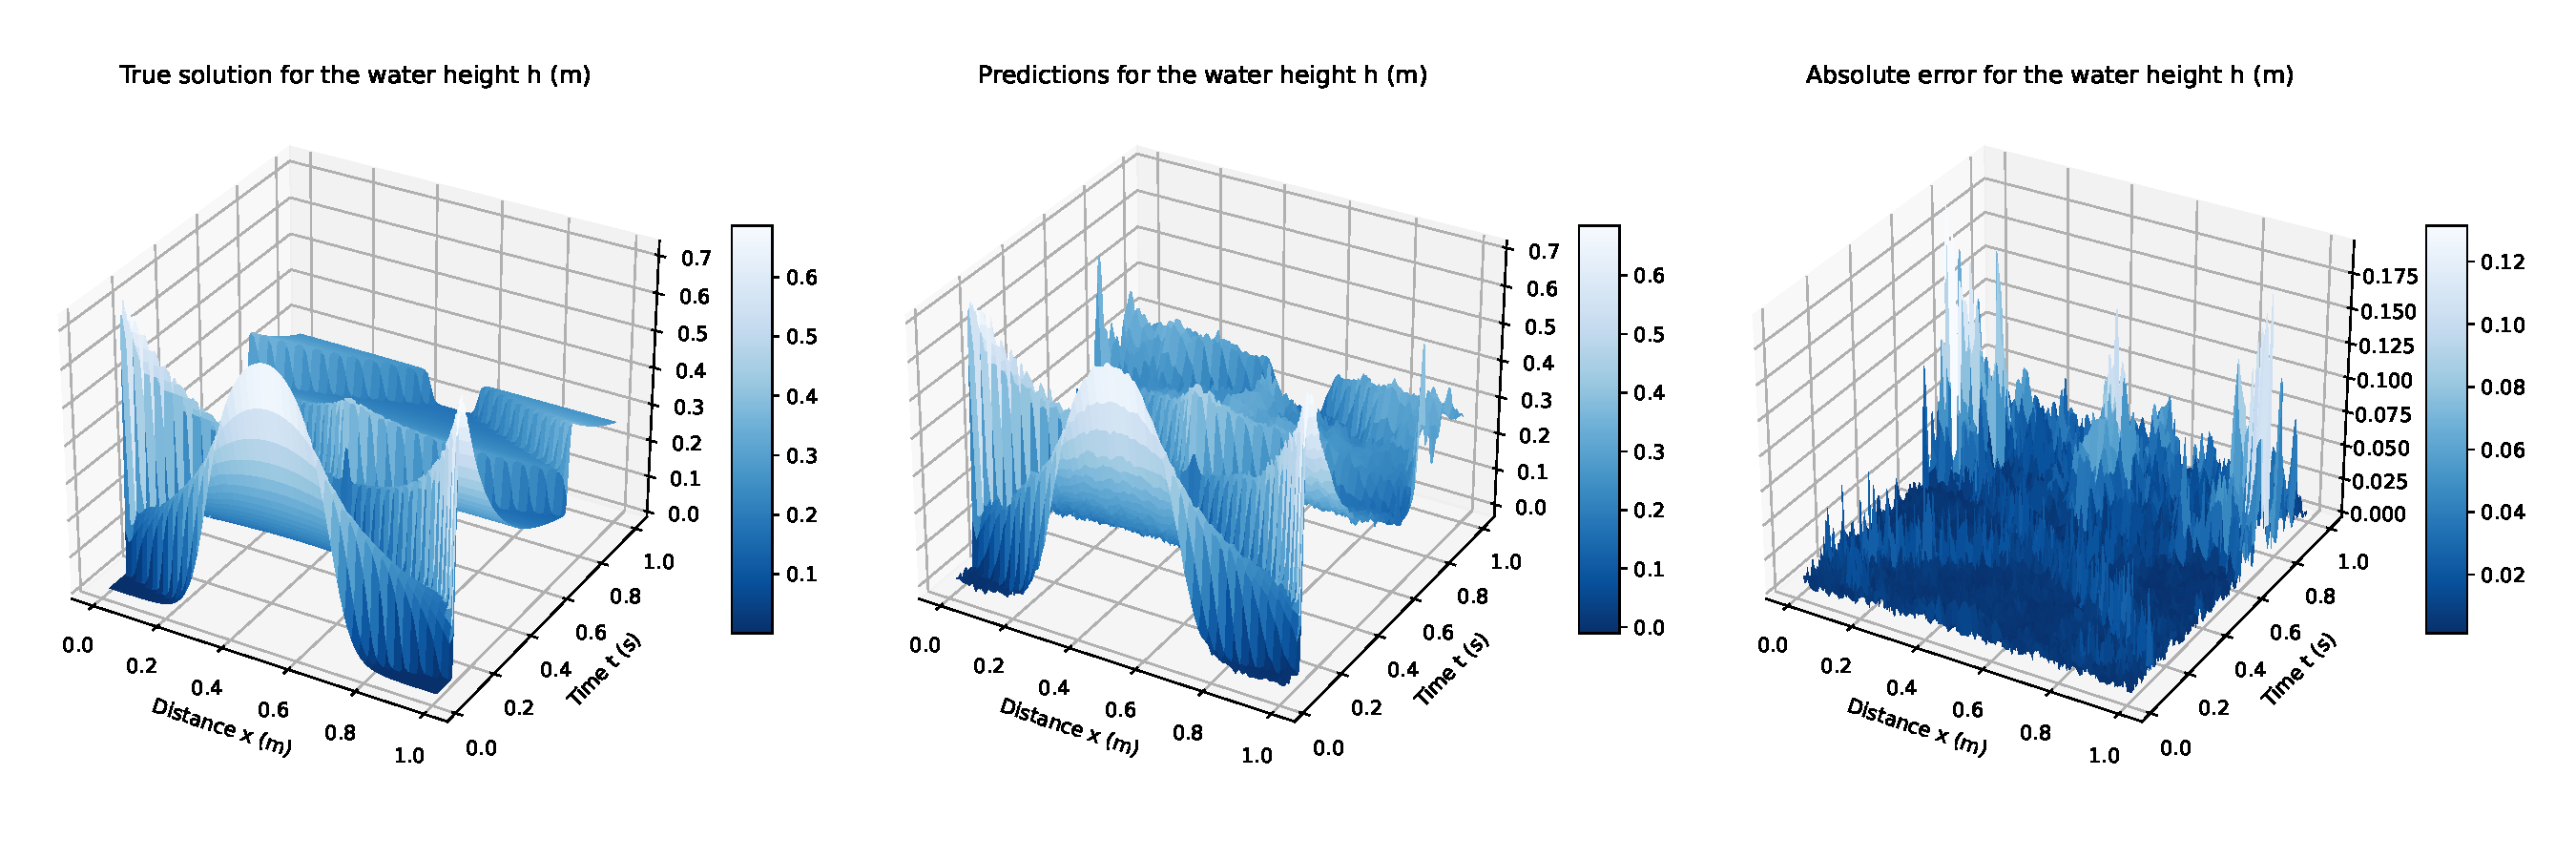
\includegraphics[width=0.99\textwidth]{C:/Users/Matteo/Shallow-Water-Equations/plots/NN_predictions.pdf}
    \caption{Predictions.}\label{fig:NN_predictions}
\end{figure}
From \autoref{fig:NN_predictions} we see that the neural network, is able to learn the dynamics of the solution, but the predictions are not accurate enough.
We also see that the highest absolute errors are located at the edges of the solution, which is expected, as the solution tends to be discontinuous.
We also see that the further we get in time, the worse the predictions become. This is also somehow expected, since we are outside the training data.
The training and validation loss is shown in \autoref{fig:NN_loss_train_val}.
\begin{figure}[H]
    \centering
    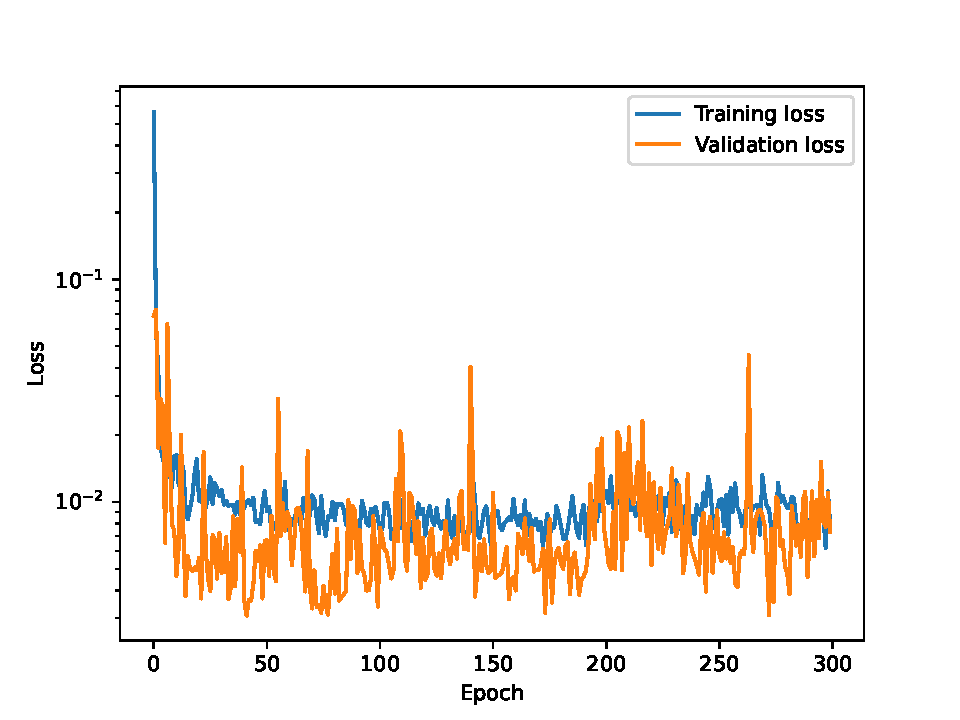
\includegraphics[width=0.6\textwidth]{C:/Users/Matteo/Shallow-Water-Equations/plots/NN_loss_train_val.pdf}
    \caption{Training and validation loss.}\label{fig:NN_loss_train_val}
\end{figure}
From \autoref{fig:NN_loss_train_val}, we see that a higher number of epochs, would probably not be beneficial, as the validation loss is increasing after a certain number of epochs.
Based on the training and validation loss, the model is overfitting the data. We see that as the training loss is decreasing, the validation loss is increasing.
This also means that the model is not able to generalize the data.
A possible solution could be to use more data.
To understand the performance of the model, we consider the predictions for some given time steps, shown in \autoref{fig:NN_predictions_time_steps}.
\begin{figure}[H]
    \centering
    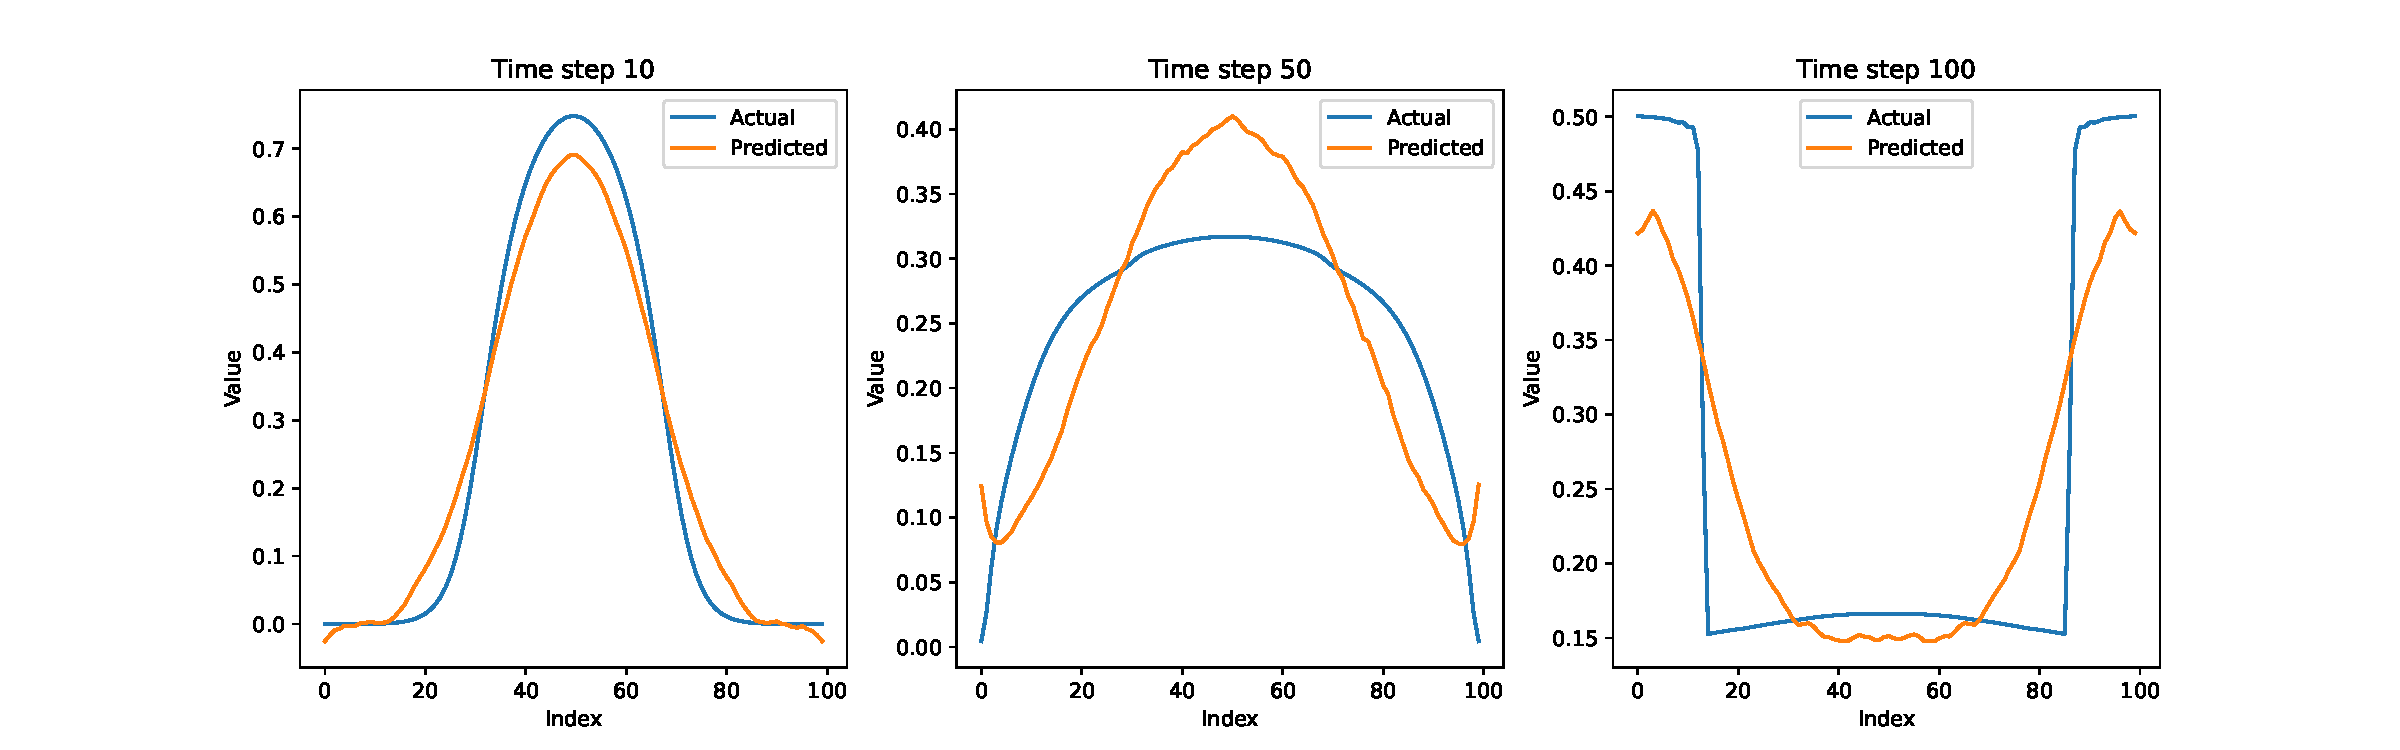
\includegraphics[width=0.95\textwidth]{C:/Users/Matteo/Shallow-Water-Equations/plots/NN_predictions_time_steps.pdf}
    \caption{Predictions for some given time steps.}\label{fig:NN_predictions_time_steps}
\end{figure}
Again, we see that the model finds some of the dynamics, but has many oscillations.
We have also trained a FNN model and a LSTM model, but the results are not shown here, as the performance is worse than the RNN model.


\subsection{FNO}
One of the main goals in this thesis is to use Fourier Neural Operators to solve the shallow water equations.
We define a FNO model, which consists of an input channel, 64 hidden channels and an output channel. We use a Fourier basis with 16 modes and a batch size of 32.
The model is trained using the Adam optimizer with a learning rate of $0.001$, a total of $1000$ epochs and the critera is to minimize the mean squared error (MSE).
The model is trained on the same data as the RNN model, and tested on the same data.
The results of the model are shown in \autoref{fig:FNO_predictions}.
\begin{figure}[H]
    \centering
    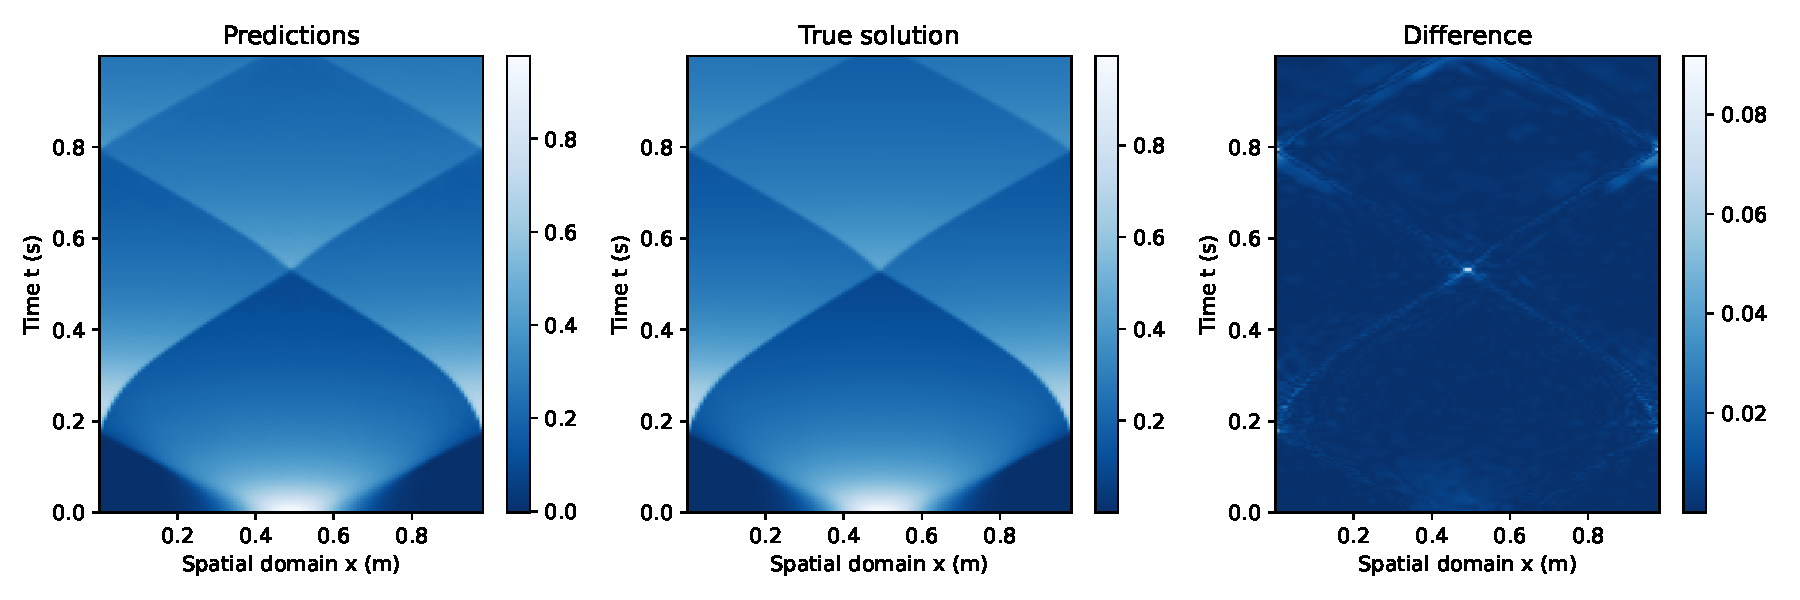
\includegraphics[width=0.9\textwidth]{C:/Users/Matteo/Shallow-Water-Equations/plots/pred_swe_epochs1000_channels64_lr_0.001.pdf}
    \caption{FNO predictions.}\label{fig:FNO_predictions}
\end{figure}
From \autoref{fig:FNO_predictions} we see that the FNO model is able to learn the dynamics of the solution, and it is able to predict the solution with high accuracy.
From the figure we also see that the error follows the edges of the solution, which is expected, as the solution tends to be discontinuous.
The loss for each iteration, which is epochs $\times$ batches, is shown in \autoref{fig:FNO_loss}.
\begin{figure}[H]
    \centering
    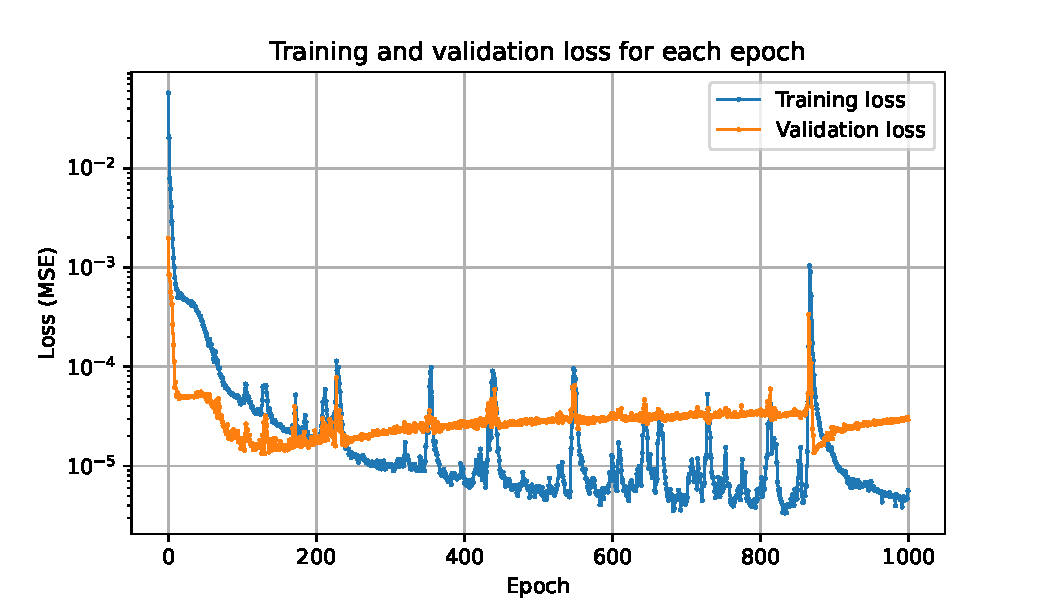
\includegraphics[width=0.7\textwidth]{C:/Users/Matteo/Shallow-Water-Equations/plots/loss_swe_epochs1000_channels64_lr_0.001.pdf}
    \caption{FNO loss.}\label{fig:FNO_loss}
\end{figure}
From \autoref{fig:FNO_loss} we see that the loss is decreasing for each iteration, and the model is able to learn the dynamics of the solution.
To get a deeper understanding of the performance of the model, we consider the predictions for some given time steps, shown in \autoref{fig:FNO_predictions_time_steps}.
\begin{figure}[H]
    \centering
    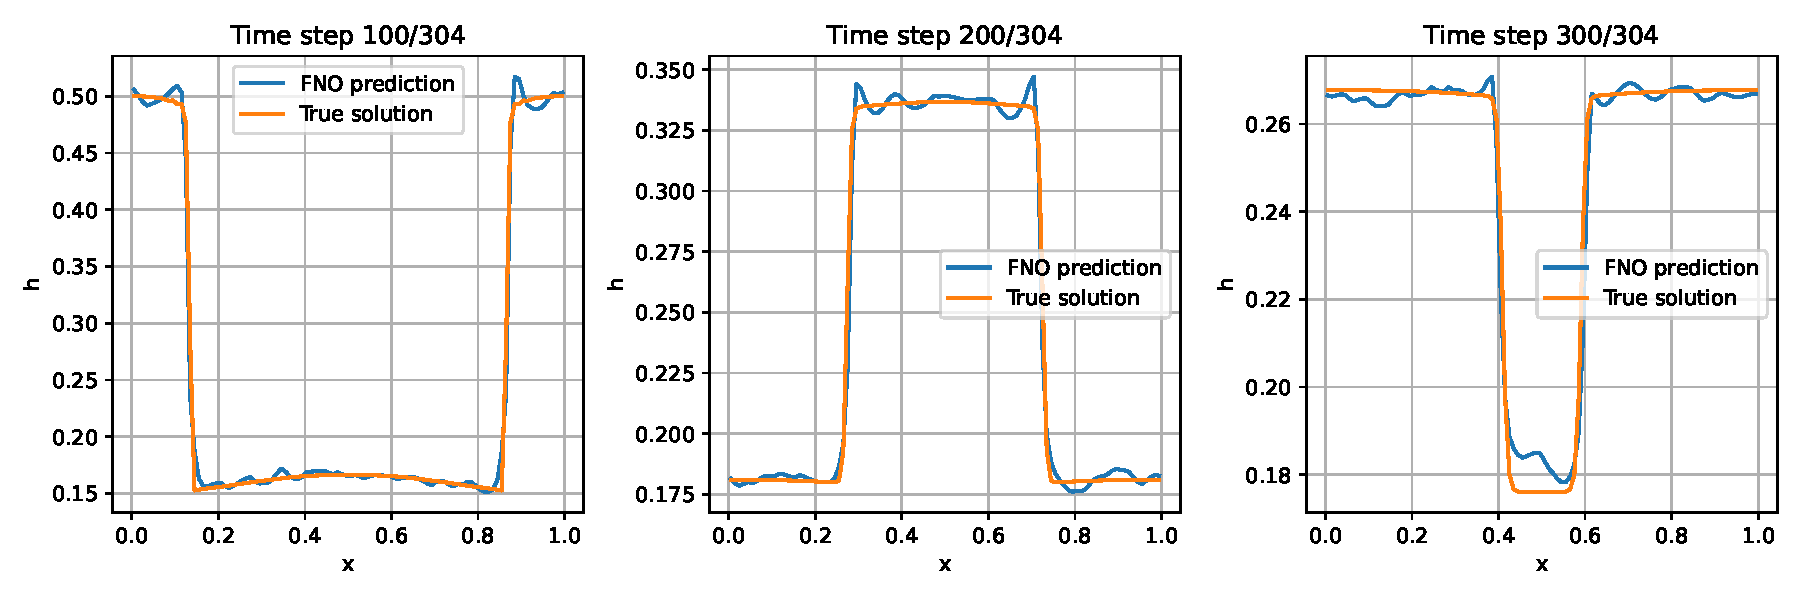
\includegraphics[width=0.9\textwidth]{C:/Users/Matteo/Shallow-Water-Equations/plots/pred_swe_epochs1000_channels64_lr_0.001_timesteps.pdf}
    \caption{FNO predictions timesteps.}\label{fig:FNO_predictions_time_steps}
\end{figure}
\autoref{fig:FNO_predictions_time_steps} demonstrates that the predictions effectively capture the solution's dynamics.
The RMSE for the predictions is shown in \autoref{fig:FNO_rmse}.
\begin{figure}[H]
    \centering
    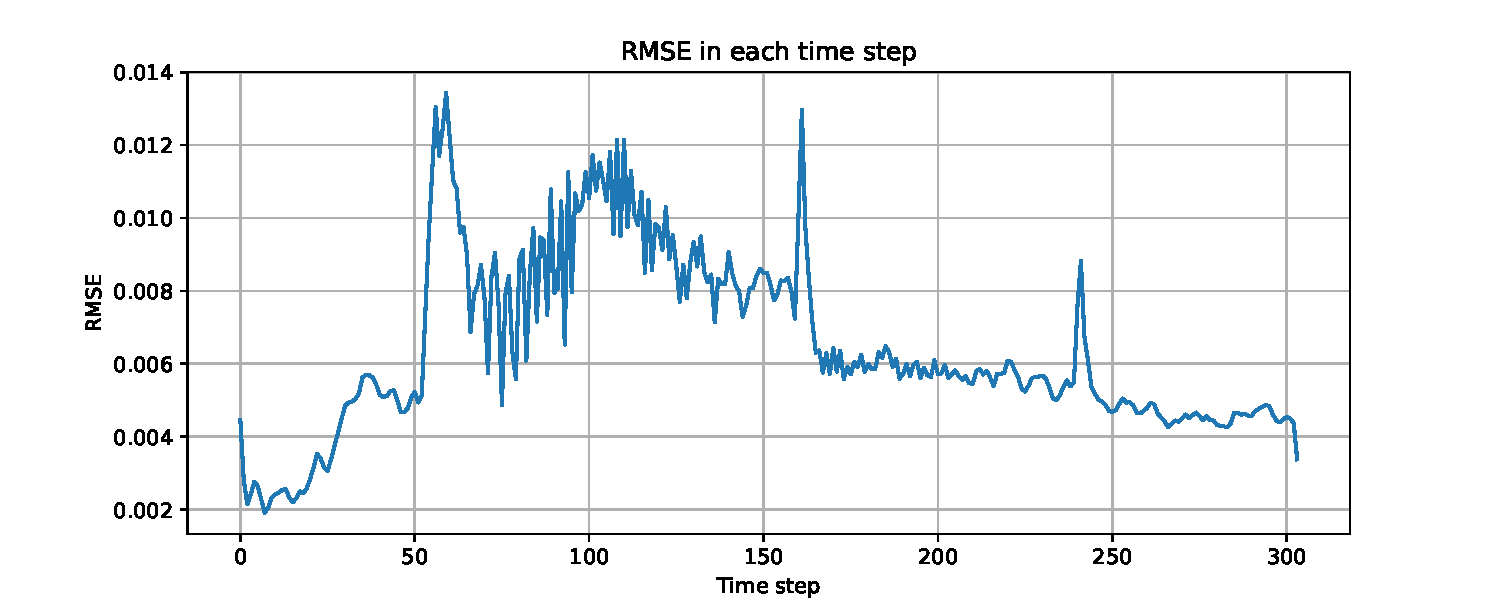
\includegraphics[width=0.7\textwidth]{C:/Users/Matteo/Shallow-Water-Equations/plots/rmse_swe_epochs1000_channels64_lr_0.001.pdf}
    \caption{FNO predictions RMSE.}\label{fig:FNO_rmse}
\end{figure}
From \autoref{fig:FNO_rmse} we see that the RMSE is not increasing for the predictions, which is a good sign.


\subsubsection{FNO Toro test 1}
To test the FNO model on a more challenging problem, we consider the Toro test case 1.
We use the same model as before, but we train it on the data from the Toro test case 1.
Again, we use the first $80\%$ of the data for training and the last $20\%$ for testing.
The results of the model are shown in \autoref{fig:FNO_Toro_test1_predictions_3D} and \autoref{fig:FNO_Toro_test1_predictions}.

\begin{figure}[H]
    \centering
    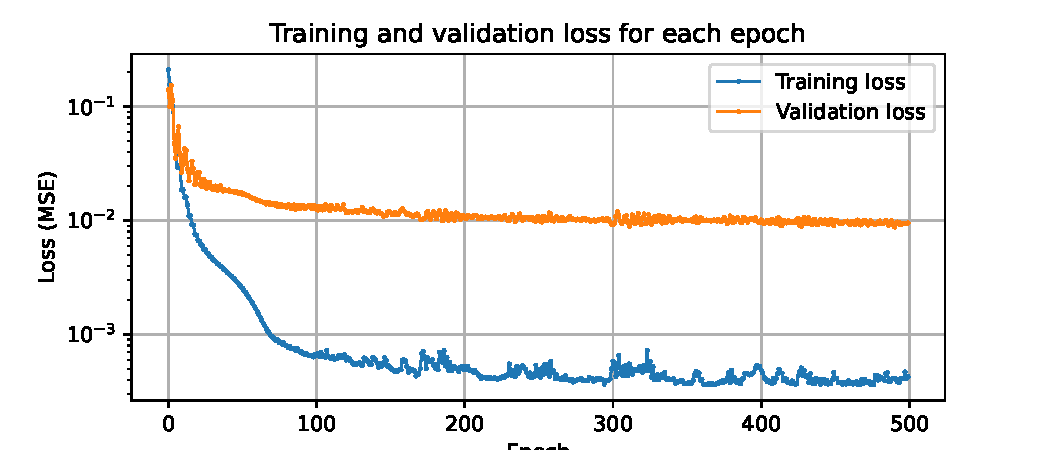
\includegraphics[width=0.7\textwidth]{C:/Users/Matteo/Shallow-Water-Equations/plots/torotest1_loss.pdf}
    \caption{FNO Toro test 1 loss.}\label{fig:FNO_Toro_test1_loss}
\end{figure}

\begin{figure}[H]
    \centering
    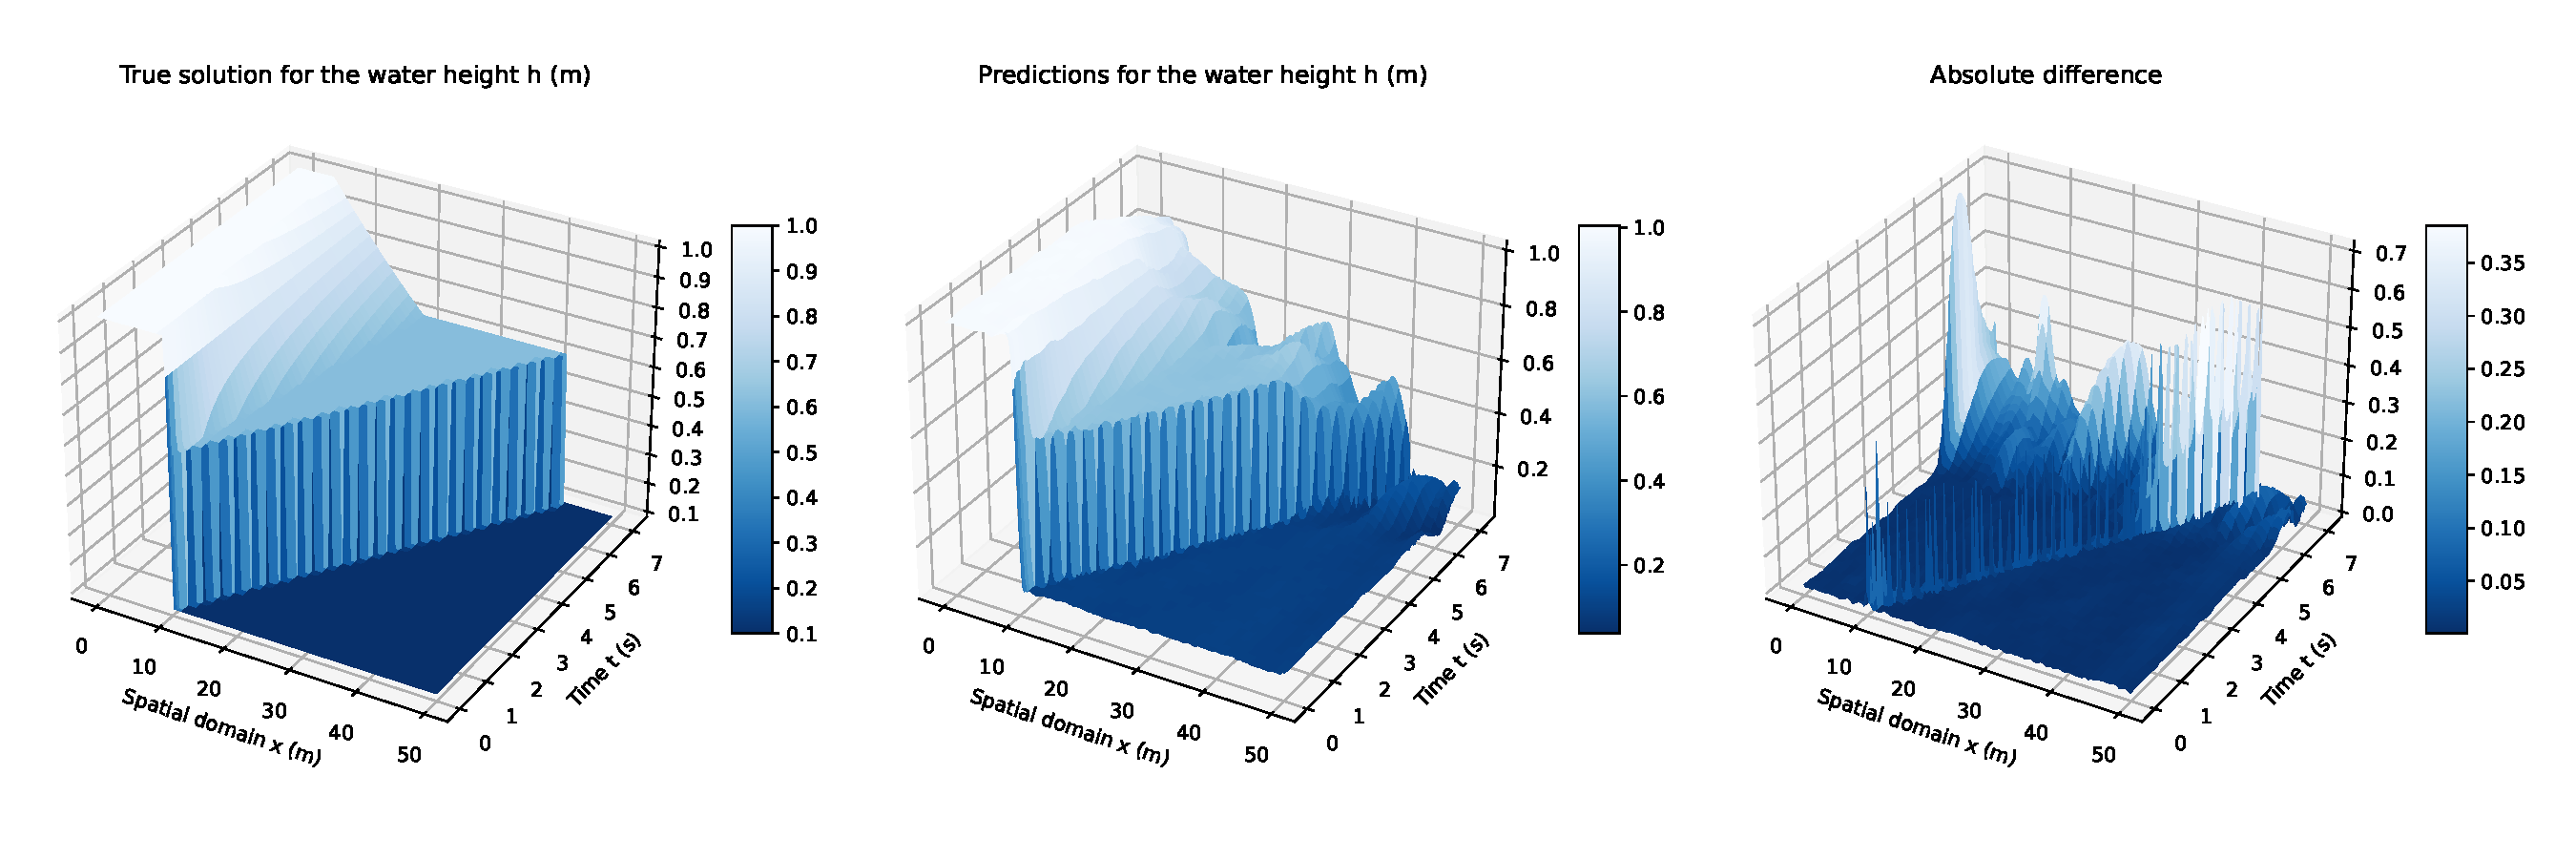
\includegraphics[width=0.9\textwidth]{C:/Users/Matteo/Shallow-Water-Equations/plots/torotest1_predictions_3D.pdf}
    \caption{FNO Toro test 1 predictions in 3d.}\label{fig:FNO_Toro_test1_predictions_3D}
\end{figure}


\begin{figure}[H]
    \centering
    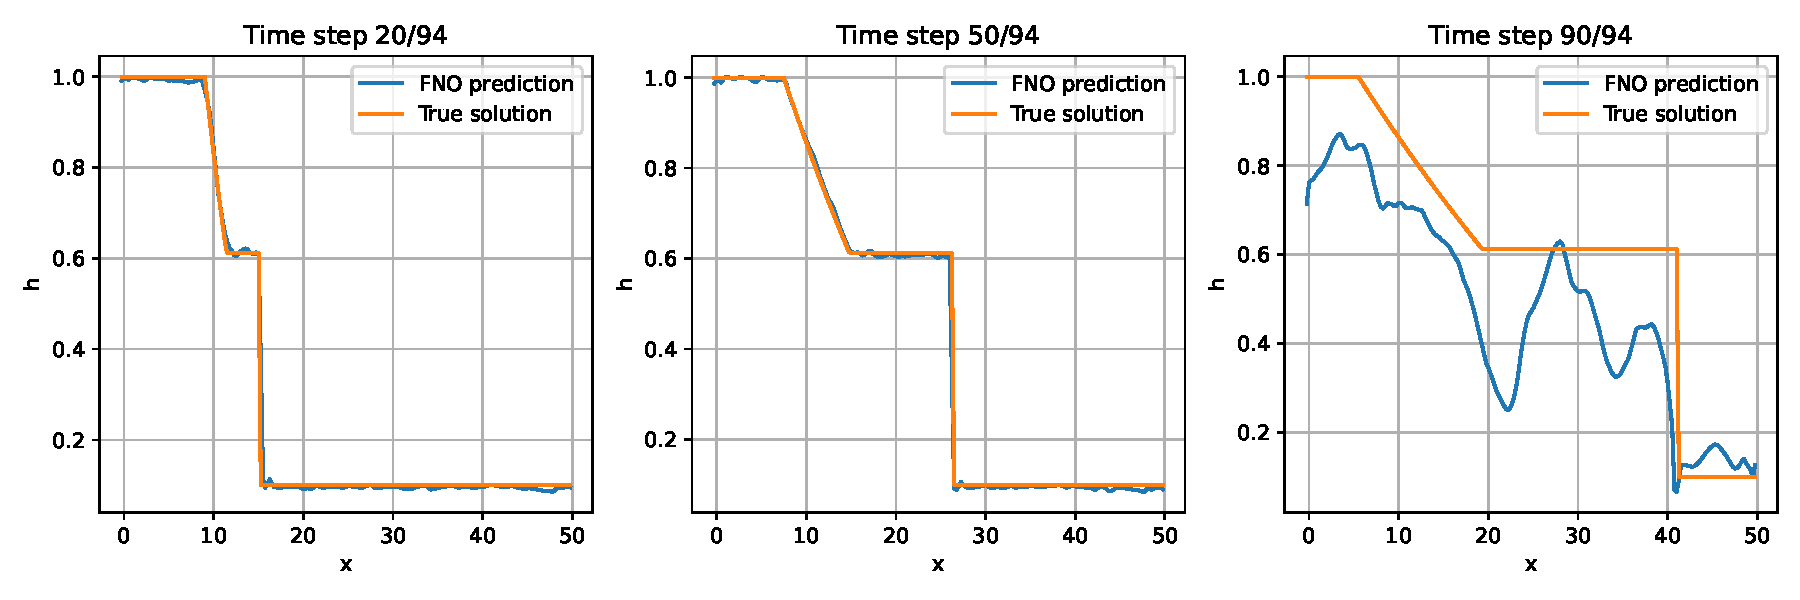
\includegraphics[width=0.9\textwidth]{C:/Users/Matteo/Shallow-Water-Equations/plots/torotest1_predictions_time_steps.pdf}
    \caption{FNO Toro test 1 predictions timesteps.}\label{fig:FNO_Toro_test1_predictions_time_steps}
\end{figure}


\begin{figure}[H]
    \centering
    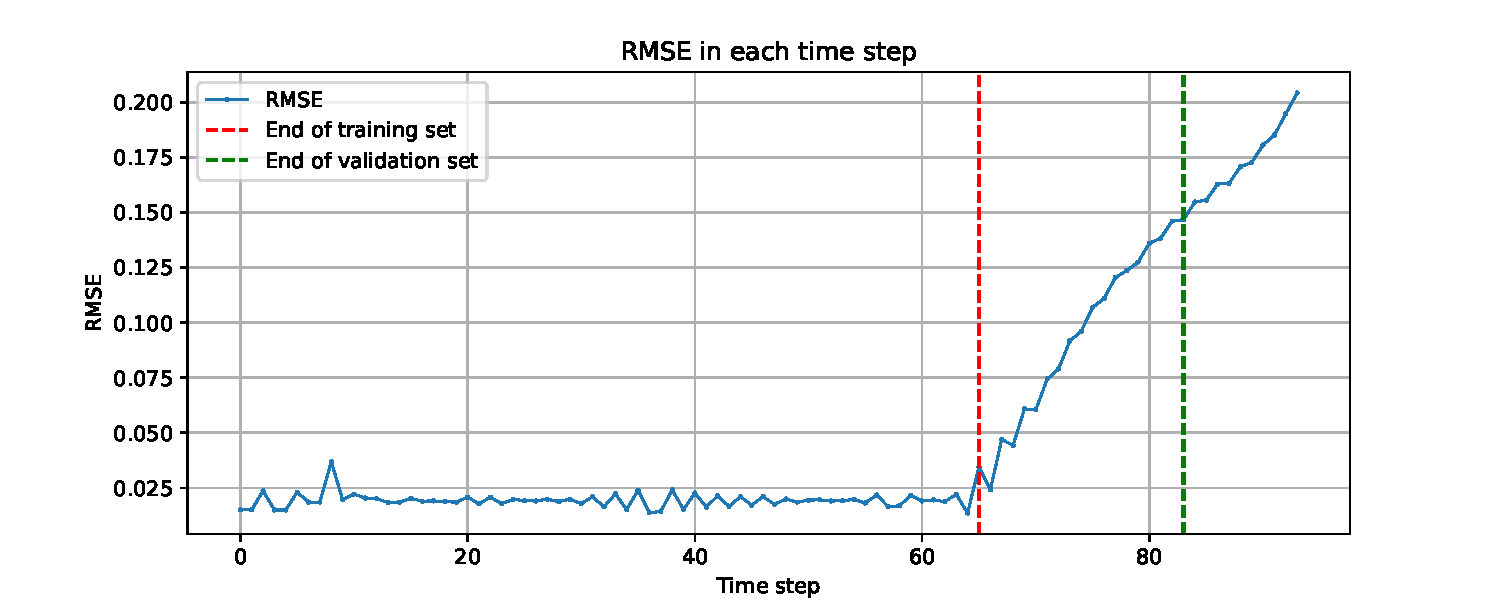
\includegraphics[width=0.7\textwidth]{C:/Users/Matteo/Shallow-Water-Equations/plots/torotest1_RMSE.pdf}
    \caption{FNO Toro test 1 predictions RMSE.}\label{fig:FNO_Toro_test1_rmse}
\end{figure}

\subsection{Spherical SWE in 1D}
We also consider the spherical shallow water equations in 1D.
Meaning we consider the linearized SWE on a circle.
The initial conditions can be seen in \autoref{fig:swe_spherical_1d_initial_conditions}.
\begin{figure}[H]
    \centering
    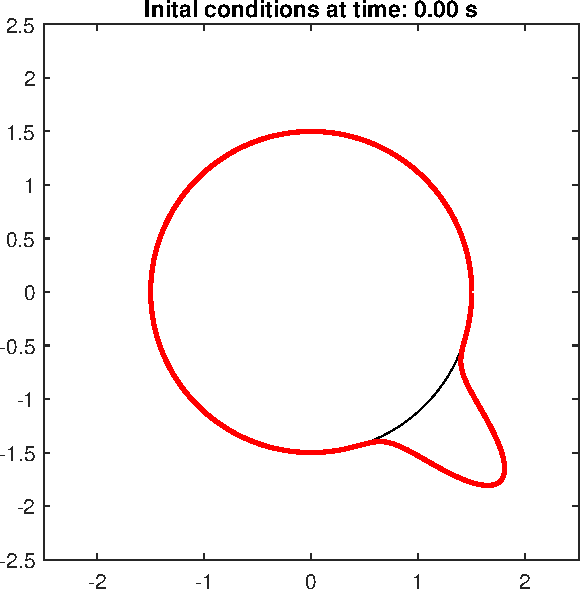
\includegraphics[width=0.4\textwidth]{C:/Users/Matteo/Shallow-Water-Equations/plots/SWE-spherical-1d-initial_conditions.pdf}
    \caption{Initial conditions for the 1D linearized shallow water equations in spherical coordinates.}\label{fig:swe_spherical_1d_initial_conditions}
\end{figure}
We have trained a FNO model on the data generated by the numerical solution of the SWE in 1D.
The numerical solution in the 




\begin{figure}[H]
    \centering
    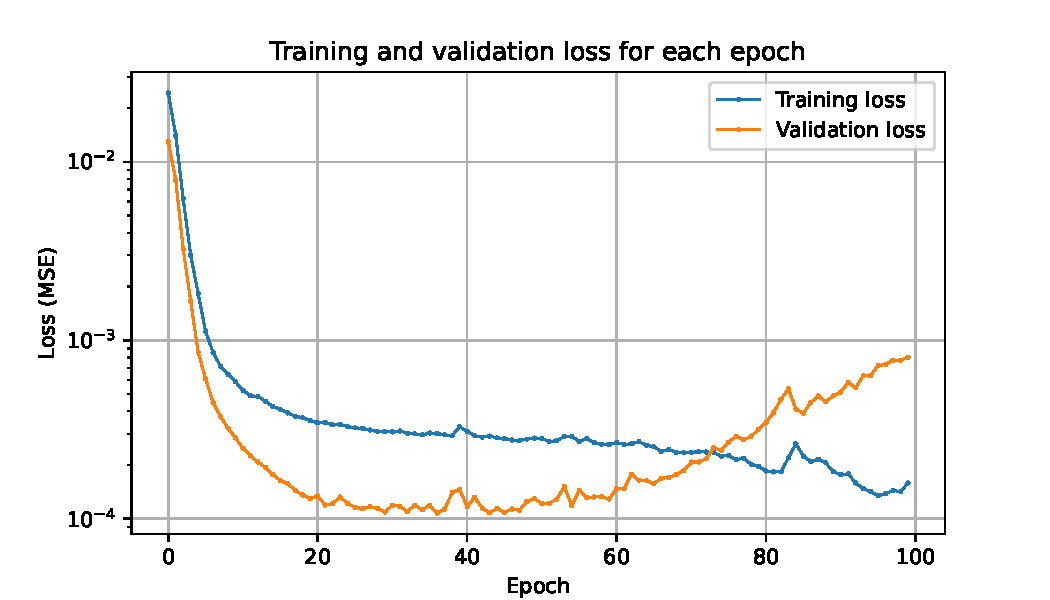
\includegraphics[width=0.7\textwidth]{C:/Users/Matteo/Shallow-Water-Equations/plots/Spherical_linear_1D_FNO.pdf}
    \caption{Numerical solution of the spherical shallow water equations in 1D.}\label{fig:Spherical_linear_1D}
\end{figure}

\begin{figure}[H]
    \centering
    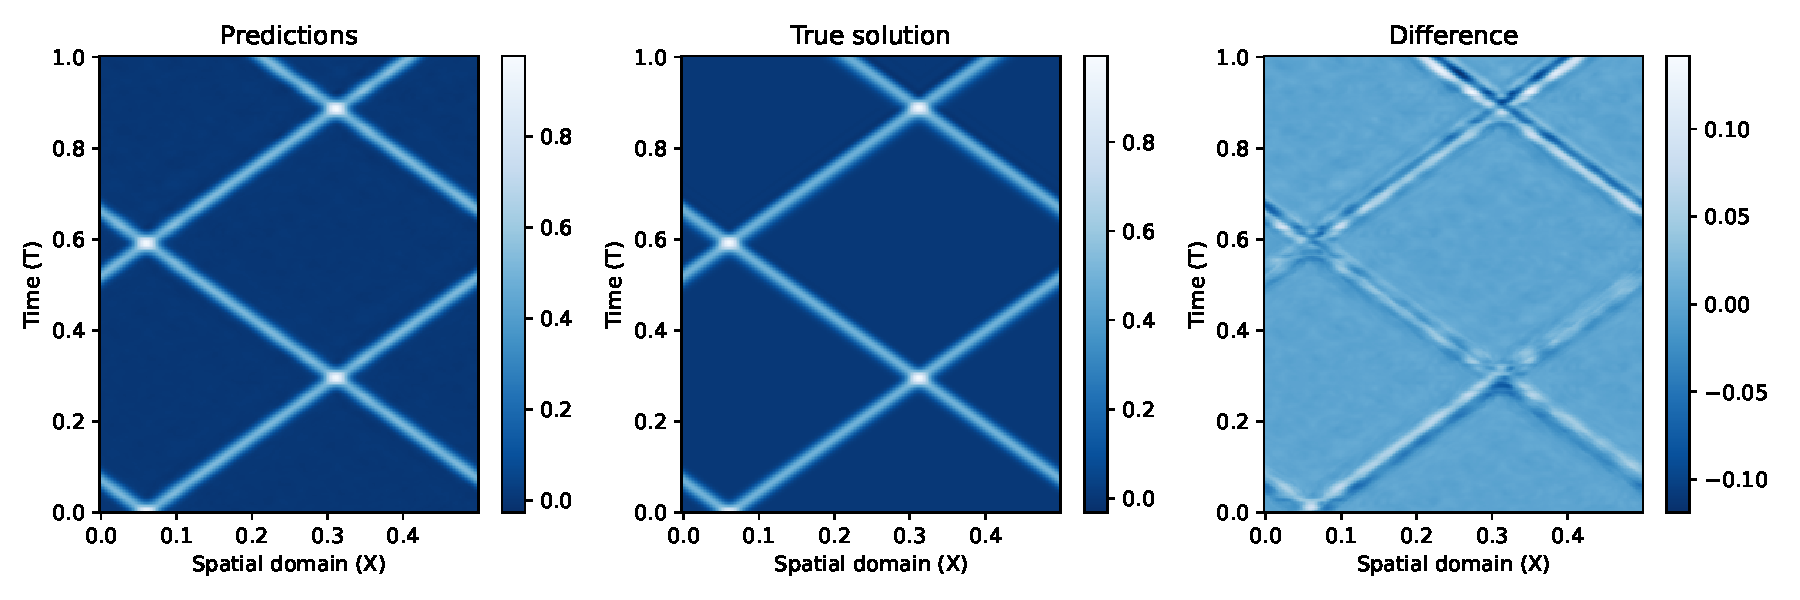
\includegraphics[width=0.7\textwidth]{C:/Users/Matteo/Shallow-Water-Equations/plots/Spherical_linear_1D_FNO_predictions.pdf}
    \caption{Predictions for the spherical shallow water equations in 1D.}\label{fig:Spherical_linear_1D_FNO_predictions}
\end{figure}

\begin{figure}[H]
    \centering
    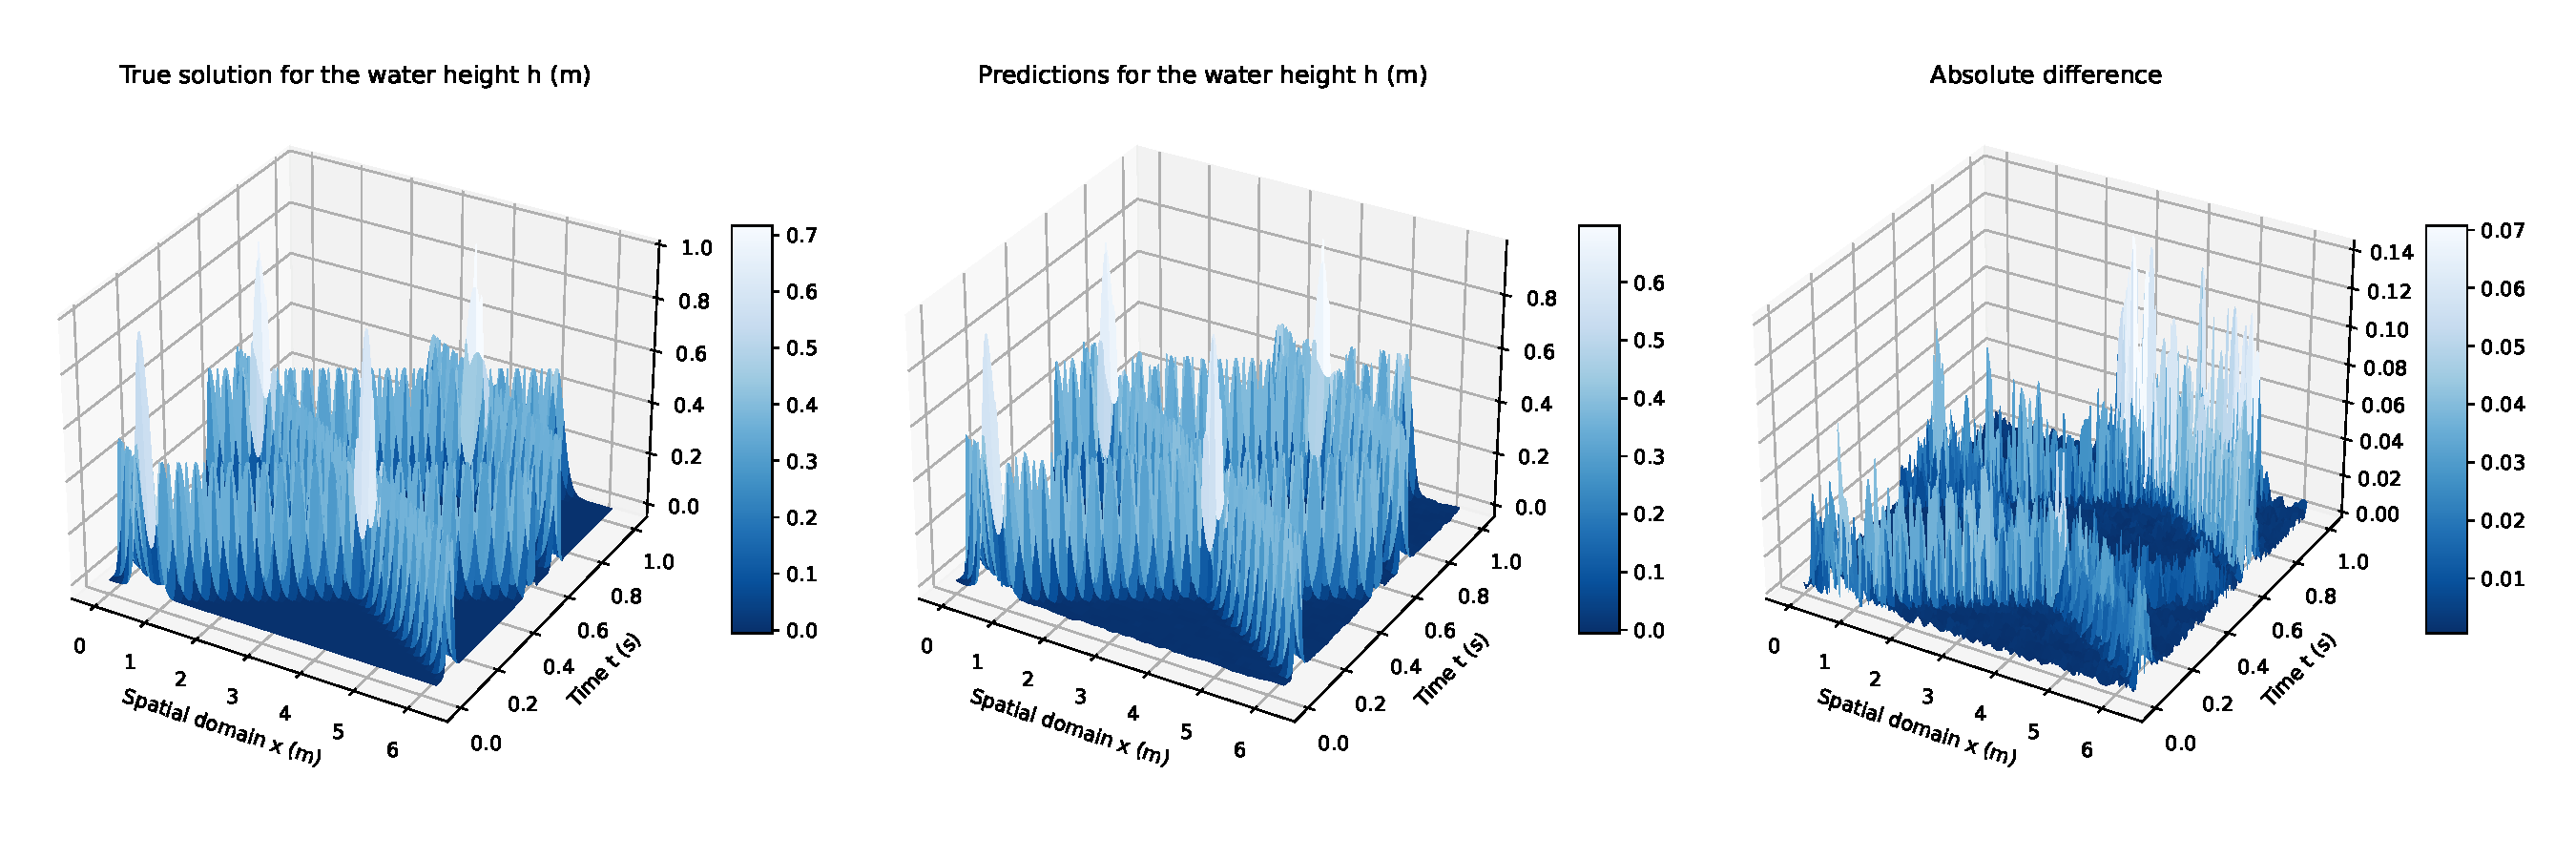
\includegraphics[width=0.7\textwidth]{C:/Users/Matteo/Shallow-Water-Equations/plots/Spherical_linear_1D_FNO_predictions_3D.pdf}
    \caption{Predictions for the spherical shallow water equations in 1D.}\label{fig:Spherical_linear_1D_FNO_predictions_3D}
\end{figure}

\begin{figure}[H]
    \centering
    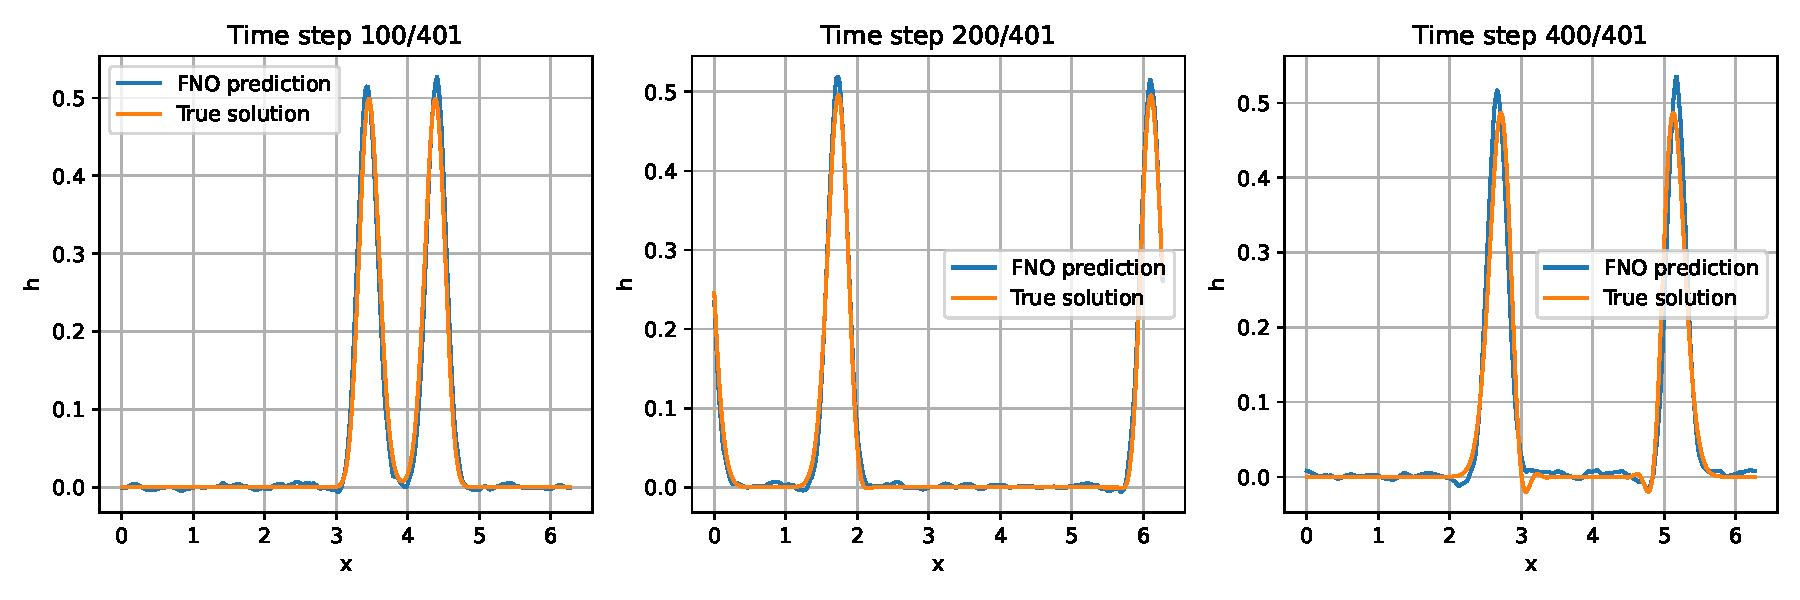
\includegraphics[width=0.7\textwidth]{C:/Users/Matteo/Shallow-Water-Equations/plots/Spherical_linear_1D_FNO_timesteps.pdf}
    \caption{Predictions for the spherical shallow water equations in 1D.}\label{fig:Spherical_linear_1D_FNO_predictions_timesteps}
\end{figure}


\begin{figure}[H]
    \centering
    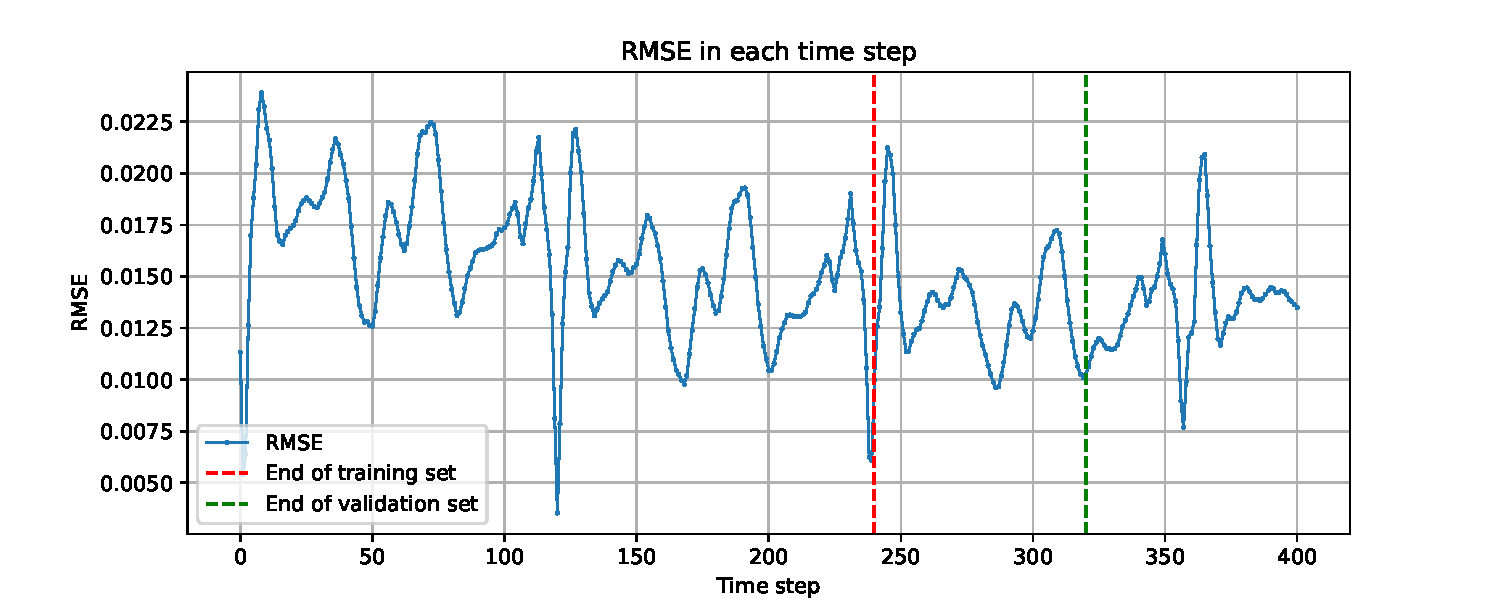
\includegraphics[width=0.7\textwidth]{C:/Users/Matteo/Shallow-Water-Equations/plots/Spherical_linear_1D_FNO_RMSE.pdf}
    \caption{RMSE for the predictions for the spherical shallow water equations in 1D.}\label{fig:Spherical_linear_1D_FNO_RMSE}
\end{figure}



\subsection{Comparison}
To get an overview of the performance of the different models, we consider the RMSE for the predictions for the smooth case.
We consider the MSE for the whole data set, and the time for training the model.
\begin{table}[H]
    \centering
    \begin{tabular}{c|c|c}
        \hline
        \text{Model} & \text{MSE} & \text{Time}\\
        \hline\hline
        \text{RNN} & $8.71 \cdot 10^{-4}$ &  464.13 s \\ 
        \hline
        \text{FNO} & $3.70 \cdot 10^{-6}$ & 383.60 s  \\
        \hline
    \end{tabular}
    \caption{MSE and time for training the models for the smooth case.}\label{tab:RMSE_smooth}
\end{table}

\begin{table}[H]
    \centering
    \begin{tabular}{c|c|c}
        \hline
        \text{Model} & \text{MSE} & \text{Eval time} \\
        \hline\hline
        \text{RNN} &  &  \\ 
        \hline
        \text{FNO} &  &  \\
        \hline
    \end{tabular}
    \caption{RMSE and evalutation time for the predictions for the Toro test case 1.}\label{tab:torotest1}
\end{table}










\section{2D Shallow Water Equations with Gaussian initial conditions}\label{sec:data-driven-results-2D}
In this section we present the results for the 2D SWE using data-driven models. 
The initial condition, a Gaussian function, is the same as in the 1D case but extended to two dimensions.
We solve the 2D SWE using both a CNN and and FNO model, comparing their performance in terms of run time and accuracy.
Additionally, we compare their run time to the FVM to evaluate whether the data-driven models can serve as a faster alternative.
We also assess the models' ability to transfer solutions across grids, by training the models on a coarse grid and making predictions on a finer grid.
Finally, we evaluate the models' capability to generalize further in time, testing their long-term predictive performance.

The initial condition for the 2D problem is a Gaussian function as given in~\eqref{eq:2D_swe_ic_gaussian}.
The initial condition is illustrated in \autoref{fig:2D_gauss_initial_condition}.
\begin{figure}[H]
    \centering
    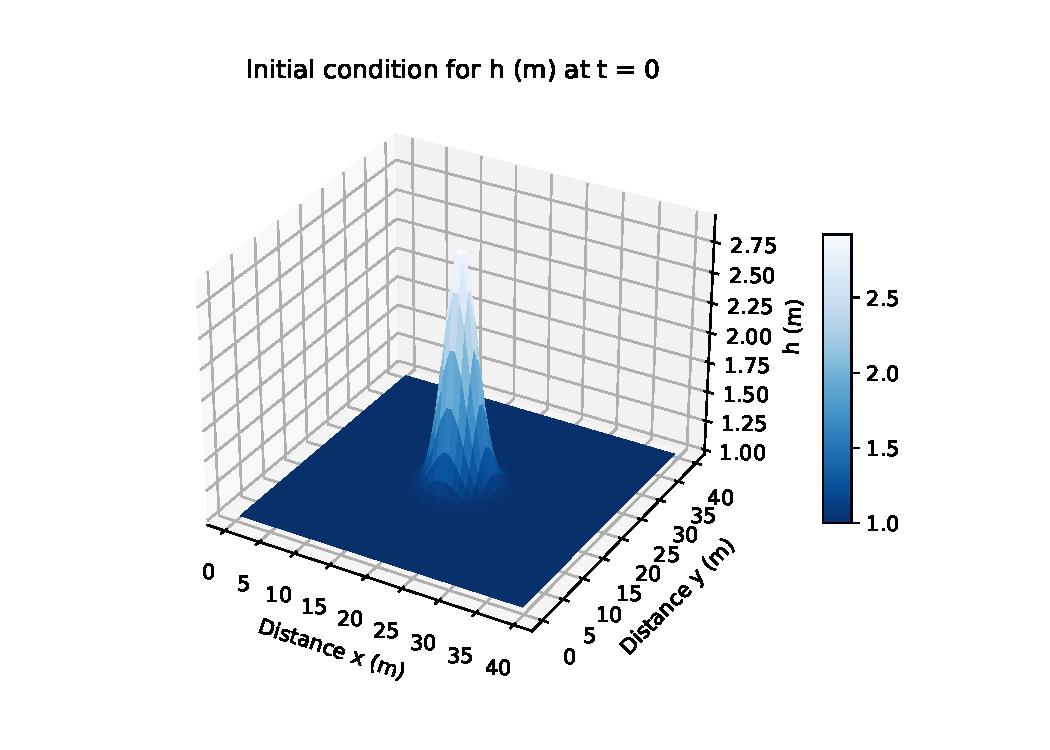
\includegraphics[width=0.6\textwidth]{C:/Users/Matteo/Shallow-Water-Equations/plots/2D_gauss_initial_condition.pdf}
    \caption{Initial condition for the 2D SWE.}\label{fig:2D_gauss_initial_condition}
\end{figure}
In \autoref{fig:2D_gauss_initial_condition} we see the initial condition for the 2D SWE problem, which is close to the 2D dam break problem, only here with a Gaussian function.
The solution is generated from $t = 0$ to $t = 5$ s.
Some information of the data used for the 2D SWE generated by the FVM can be found in \autoref{tab:data_2D_SWE}.
\begin{table}[H]
    \centering
    \begin{tabular}{c|ccccc}
        \textbf{Case} & \textbf{n\_train} & \textbf{n\_val} & \textbf{n\_test} & $\mathbf{\Delta x}$ & $\mathbf{\Delta t}$ \\
        \hline
        2D SWE, N = 64 & 48 & 16 & 17 & 0.625 m  & $[0.050 \text{ s}, 0.073 \text{ s}]$ \\
        2D SWE, N = 128 & 99 & 33 & 33 & 0.3125 m  & $[0.025 \text{ s}, 0.035 \text{ s}]$ \\
    \end{tabular}
    \caption{Details of the used data for the case with the 2D SWE for both a number of grid points $N=64$ and $N=128$.}\label{tab:data_2D_SWE}
\end{table}
In \autoref{tab:data_2D_SWE} we see that the train/validation/test data split is $60\%/20\%/20\%$ for both $N = 64$ and $N = 128$.
In the FVM we use a variable time step size $\Delta t$ to ensure stability, which is why the time step size varies.
We see that for $N = 64$ the time step size varies between $0.050$ s and $0.073$ s, while for $N = 128$ the time step size varies between $0.025$ s and $0.035$ s.
The time step size for the higher $N$ is in general smaller than for the lower $N$ to ensure stability.
This is also what gives more data points for $N = 128$ compared to $N = 64$.


\subsubsection*{CNN Model}
We train a CNN model with several convolutional layers and ReLU activation functions.
We use the Adam optimizer with a learning rate of $0.001$ and a batch size of $32$.
We make predictions from $t = 0$ to $t = 5$.
The model is trained for $500$ epochs.
The training and validation loss for the 2D CNN model can be seen in \autoref{fig:2D_CNN_loss}.
\begin{figure}[H]
    \centering
    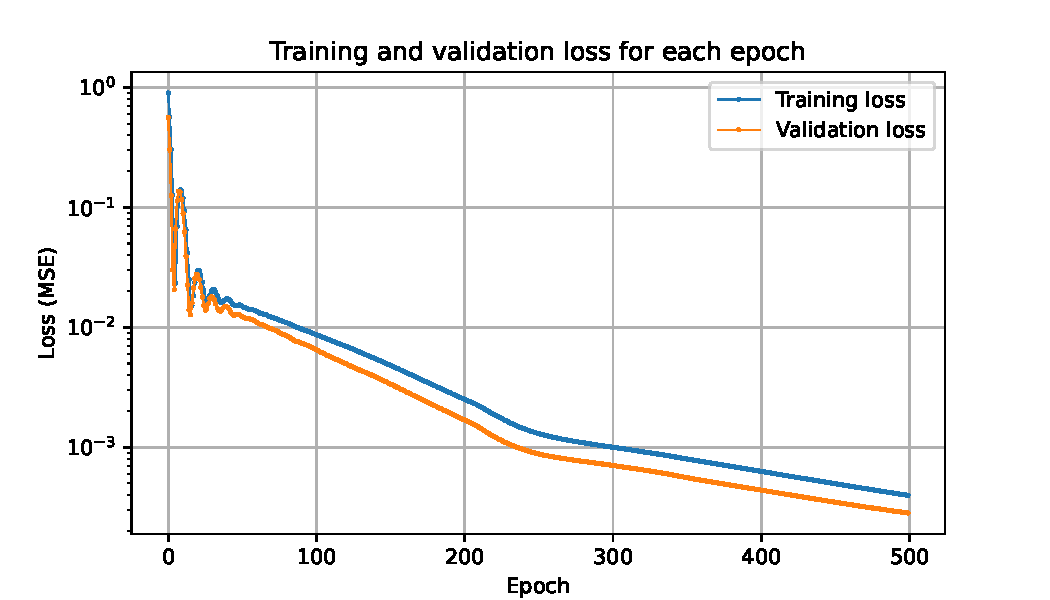
\includegraphics[width=0.7\textwidth]{C:/Users/Matteo/Shallow-Water-Equations/plots/2D_CNN_loss.pdf}
    \caption{Training and validation loss for the 2D CNN model.}\label{fig:2D_CNN_loss}
\end{figure}
\autoref{fig:2D_CNN_loss} shows that the training and validation loss are decreasing, as a function of the number of epochs.
The error plot for the last prediction for the 2D CNN can be seen in \autoref{fig:2D_CNN_error}.
\begin{figure}[H]
    \centering
    \includegraphics[width=0.95\textwidth]{C:/Users/Matteo/Shallow-Water-Equations/plots/2D_CNN_error.pdf}
    \caption{Error plot for the last prediction for the 2D CNN.}\label{fig:2D_CNN_error}
\end{figure}
From \autoref{fig:2D_CNN_error}, we see that overall the absolute error is small.
The error is largest at the boundaries of the domain. 
This may be due to the fact that in this case we are working with boundary conditions simulating a wall.
Hence, when the wave hits the wall, the wave is reflected, and the model has to learn the reflection of the wave.
This may also lead to discontinuities in the solution, which can be difficult for the model to handle.

\subsubsection*{FNO Model}
We train a FNO model with the same training/validation/testing split as for the CNN model.
The FNO model uses 8 Fourier modes, the Adam optimizer with a learning rate of $0.001$, and a batch size of $10$.
The model is trained for $500$ epochs.
The training and validation loss for the 2D FNO model can be seen in \autoref{fig:2D_FNO_loss}.
\begin{figure}[H]
    \centering
    \includegraphics[width=0.7\textwidth]{C:/Users/Matteo/Shallow-Water-Equations/plots/2D_FNO_loss.pdf}
    \caption{Training and validation loss for the 2D FNO model.}\label{fig:2D_FNO_loss}
\end{figure}
From \autoref{fig:2D_FNO_loss} we see that the training and validation loss are decreasing, and more or less stable with some fluctations. 
The plot suggests that the model has converged.
The error plot for the last prediction for the 2D FNO can be seen in \autoref{fig:2D_FNO_error}.
\begin{figure}[H]
    \centering
    \includegraphics[width=0.95\textwidth]{C:/Users/Matteo/Shallow-Water-Equations/plots/2D_FNO_error.pdf}
    \caption{Error plot for the last prediction for the 2D FNO.}\label{fig:2D_FNO_error}
\end{figure}
As for the CNN model, the error is largest at the boundaries.
However, we notice that the absolute error is smaller for the FNO model compared to the CNN model.

\subsubsection*{Comparison}
We compare the performance of the CNN and FNO models in terms of the MSE and MAE for the predictions.
We test for both $N = 64$ and $N = 128$ grid points in each direction.
The errors are calculated for the test data, i.e., the last $20\%$ of the time steps.
The results are summarized in \autoref{tab:results_2D_comparison}, together with the time for training the models.
\begin{table}[H]
    \centering
    \small % Reduce font size
    \begin{tabular}{c|cccc|cccc}
        Model & \multicolumn{4}{c|}{$N = 64$} & \multicolumn{4}{c}{$N = 128$} \\
        \cline{2-9}
        & Epochs & MSE & MAE & Time (s) & Epochs & MSE & MAE & Time (s) \\
        \hline
        CNN  &
        \input{C:/Users/Matteo/Shallow-Water-Equations/saved_results/2D_CNN_Nx=64_nepochs.txt} &
        \input{C:/Users/Matteo/Shallow-Water-Equations/saved_results/2D_CNN_Nx=64_MSE_test.txt} & 
        \input{C:/Users/Matteo/Shallow-Water-Equations/saved_results/2D_CNN_Nx=64_MAE_test.txt} &
        \input{C:/Users/Matteo/Shallow-Water-Equations/saved_results/2D_CNN_Nx=64_time.txt} &
        \input{C:/Users/Matteo/Shallow-Water-Equations/saved_results/2D_CNN_Nx=128_nepochs.txt} &
        \input{C:/Users/Matteo/Shallow-Water-Equations/saved_results/2D_CNN_Nx=128_MSE_test.txt} &
        \input{C:/Users/Matteo/Shallow-Water-Equations/saved_results/2D_CNN_Nx=128_MAE_test.txt} &
        \input{C:/Users/Matteo/Shallow-Water-Equations/saved_results/2D_CNN_Nx=128_time.txt} 
        \\
        \hline
        FNO  &
        \input{C:/Users/Matteo/Shallow-Water-Equations/saved_results/2D_FNO_Nx=64_nepochs.txt} &
        \input{C:/Users/Matteo/Shallow-Water-Equations/saved_results/2D_FNO_Nx=64_MSE_test.txt} &
        \input{C:/Users/Matteo/Shallow-Water-Equations/saved_results/2D_FNO_Nx=64_MAE_test.txt} &
        \input{C:/Users/Matteo/Shallow-Water-Equations/saved_results/2D_FNO_Nx=64_time.txt} &
        \input{C:/Users/Matteo/Shallow-Water-Equations/saved_results/2D_FNO_Nx=128_nepochs.txt} &
        \input{C:/Users/Matteo/Shallow-Water-Equations/saved_results/2D_FNO_Nx=128_MSE_test.txt} &
        \input{C:/Users/Matteo/Shallow-Water-Equations/saved_results/2D_FNO_Nx=128_MAE_test.txt} &
        \input{C:/Users/Matteo/Shallow-Water-Equations/saved_results/2D_FNO_Nx=128_time.txt}
        \\
        \hline
    \end{tabular}
    \caption{Test loss in terms of MSE and MAE, and time for training the models for the 2D SWE.}\label{tab:results_2D_comparison}
\end{table}
The errors are low and similar for both models.
However, we also observe that the FNO model generally requires more time to train.
Based on theory, FNOs have demonstrated potential in transferring solutions across grids.
To test this, we train the models on a coarse grid and then make predictions on a finer grid.
The table below presents the results when the models are trained on a grid with $N = 64$ and subsequently used to make predictions on finer grids with $N = 128$ and $N = 256$.
\begin{table}[H]
    \centering
    \begin{tabular}{c|ccc|ccc}
        Model & \multicolumn{3}{c}{$N = 128$} & \multicolumn{3}{c}{$N = 256$} \\
        \cline{2-7}
        & MSE & MAE & Prediction time [s] & MSE & MAE & Prediction time [s] \\
        \hline
        CNN &
        \input{C:/Users/Matteo/Shallow-Water-Equations/saved_results/2D_CNN_train_Nx=64_test_N=128_MSE_test.txt} &
        \input{C:/Users/Matteo/Shallow-Water-Equations/saved_results/2D_CNN_train_Nx=64_test_N=128_MAE_test.txt} &
        \input{C:/Users/Matteo/Shallow-Water-Equations/saved_results/2D_CNN_train_Nx=64_test_N=128_time.txt} &
        \input{C:/Users/Matteo/Shallow-Water-Equations/saved_results/2D_CNN_train_Nx=64_test_N=256_MSE_test.txt} &
        \input{C:/Users/Matteo/Shallow-Water-Equations/saved_results/2D_CNN_train_Nx=64_test_N=256_MAE_test.txt} &
        \input{C:/Users/Matteo/Shallow-Water-Equations/saved_results/2D_CNN_train_Nx=64_test_N=256_time.txt} \\ \hline
        FNO  &
        \input{C:/Users/Matteo/Shallow-Water-Equations/saved_results/2D_FNO_train_Nx=64_test_N=128_MSE_test.txt} &
        \input{C:/Users/Matteo/Shallow-Water-Equations/saved_results/2D_FNO_train_Nx=64_test_N=128_MAE_test.txt} &
        \input{C:/Users/Matteo/Shallow-Water-Equations/saved_results/2D_FNO_train_Nx=64_test_N=128_time.txt} &
        \input{C:/Users/Matteo/Shallow-Water-Equations/saved_results/2D_FNO_train_Nx=64_test_N=256_MSE_test.txt} &
        \input{C:/Users/Matteo/Shallow-Water-Equations/saved_results/2D_FNO_train_Nx=64_test_N=256_MAE_test.txt} &
        \input{C:/Users/Matteo/Shallow-Water-Equations/saved_results/2D_FNO_train_Nx=64_test_N=256_time.txt} \\
    \end{tabular}
    \caption{Test loss in terms of MSE and MAE, and time for training the FNO model on a grid with $N = 64$ and then making predictions on a grid with $N = 128$ and $N=256$.}\label{tab:results_2D_train_64_test_128_256}
\end{table}
From the results in \autoref{tab:results_2D_train_64_test_128_256} we see that FNO model achieves small errors both for $N = 128$ and $N = 256$, indicating its ability to generalize to a finer grid.
The CNN model shows higher errors, but might still be accurate enough depending on the application.
This ability to train the FNO model (and partially, also the CNN model) on a coarse grid and make predictions on a finer grid is a significant advantage.
In htis study, it is particularly useful for solving the SWE numerically, as solving the SWE on a fine grid using the FVM is computationally expensive.
By comparing to the run time of the FVM, shown in \autoref{tab:scalability}, we see that the data-driven models are much faster, and thus, might provide an alternative to the FVM, depending on the specific application.
This approach could help the address the scalability challenges faced when solving the SWE numerically.

\subsection{Long-term predictions for the 2D Shallow Water Equations}
In this section, we evaluate the models' ability to generalize to longer time horizons.
The previous models were trained on data generated using the FVM with vairable time step sizes.
To control the specific time points for long-term predictions, a fixed time step size is required.
Consequenlty, we have generated data for the 2D SWE using $N = 64$ points in each spatial direction and a fixed time step size of $\Delta t = 0.025$ s.
To facilitate testing long-term predictions, the data set spans a longer time interval, covering $t = 0$ s to $t = 15$ s.
The models are trained on the data from $t = 0$ s to $t = 8$ s, validated on the data from $t = 8$ s to $t = 10$ s, and tested for long-term prediction capability using data from $t = 10$ s to $t = 15$ s.
Information of the data used for the 2D SWE with a fixed time step size can be found in \autoref{tab:data_2D_SWE_fixed_time_step}.
\begin{table}[H]
    \centering
    \begin{tabular}{c|ccccc}
        \textbf{Case} & \textbf{n\_train} & \textbf{n\_val} & \textbf{n\_predictions} & $\mathbf{\Delta x}$ & $\mathbf{\Delta t}$ \\
        \hline
        2D SWE & 480 & 120 & 200 & 0.625 m  & $0.025$ \\
    \end{tabular}
    \caption{Details of the used data for the case with the 2D SWE with a fixed time step size.}\label{tab:data_2D_SWE_fixed_time_step}
\end{table}
We generate predictions for up to $n = 200$ time steps into the future, corresponding to the interval from $t = 10$ s to $t = 15$ s.
The validation data points are crucial for selecting the best model for long-term predictions and prevent overfitting.
Initially, we adopted an iterative approach, where the model made a prediction for the next time step and used that prediction as input for the next time step.
While this approach produces acceptable results for the inital time steps, the error increases as we make predictions further in time, probably due to accumulating errors.
To address this issue, we implemented an alternative approach by creating sequences of data and training the model to predict the next time step based on the entire sequence.
In this method, the most recent prediction becomes part of a sequence, distributing the influence across subsequent predictions, rather than heavily impacting the next prediction alone.
This approach aims to stabilize long-term predictions.

\subsubsection*{CNN Model}
We train the CNN model on the described data set for $100$ epochs.
The model consists of several convolutional layers with ReLU activation functions.
The sequence length is set to $50$ and the model is trained using the Adam optimizer with a learning rate of $0.001$ and a batch size of $16$.
We make predictions for up to $n = 200$ time steps into the future, and the error plot for the prediction after $n = 20$ time steps, corresponding to $0.5$ s, can be seen in \autoref{fig:2D_CNN_long_term_error}.
\begin{figure}[H]
    \centering
    \includegraphics[width=\textwidth]{C:/Users/Matteo/Shallow-Water-Equations/plots/2D_CNN_long_term_predictions_error_Ntrain=64_Npred=64_idx=20.pdf}
    \caption{Error plot for the long-term prediction for the 2D CNN model.}\label{fig:2D_CNN_long_term_error}
\end{figure}
In \autoref{fig:2D_CNN_long_term_error} we see that the error is more equally distributed over the domain compared to the short-term predictions in \autoref{fig:2D_CNN_error}.
The prediction, together with the numerical solution can be seen in \autoref{fig:2D_CNN_long_term_predictions} in Appendix \autoref{app:2D_SWE_long_term_prediction}.


\subsubsection*{FNO Model}
We run the same test for the FNO model, training it on the same data set as the CNN model, and also for $100$ epochs.
The model has 12 Fourier modes and is trained using the Adam optimizer with a learning rate of $0.001$ and a batch size of $16$.
The sequence length is set to $50$.
The error plots of the long-term predictions from the FNO model after 20 time steps, equivalent to $0.5$ s, can be seen in \autoref{fig:2D_FNO_long_term_error}.
\begin{figure}[H]
    \centering
    \includegraphics[width=\textwidth]{C:/Users/Matteo/Shallow-Water-Equations/plots/2D_FNO_long_term_predictions_error_Ntrain=64_Npred=64_idx=20.pdf}
    \caption{Error plot for the long-term prediction for the 2D FNO model.}\label{fig:2D_FNO_long_term_error}
\end{figure}
From the error plot in \autoref{fig:2D_FNO_long_term_error}, we see that the error is bigger than for the short-term predictions in \autoref{fig:2D_FNO_error}, but for many applications still acceptable.
We also see that error for the FNO model is smaller than for the CNN model, indicating that the FNO model is better able to generalize further in time and make long-term predictions.
A plot of the predictions and the ground truth can be found in \autoref{fig:2D_FNO_long_term_predictions} in Appendix \autoref{app:2D_SWE_long_term_prediction}, where we see that the FNO model is able to capture the dynamics of the solution well.

\subsubsection*{Comparison}
To assess the models performance over time, we plot the error at each time step for long-term predictions up to $n = 200$ time steps into the future.
Then CNN and FNO models are compared in terms of MSE, MAE and the absolute max error for long-term predictions, as shown in \autoref{fig:2D_CNN_FNO_mse_mae_max_error}.
\begin{figure}[H]
    \centering
    \includegraphics[width=0.99\textwidth]{C:/Users/Matteo/Shallow-Water-Equations/plots/2D_CNN_FNO_mse_mae_max_error.pdf}
    \caption{MSE, MAE and max error for the long-term predictions for the 2D CNN and FNO models.}\label{fig:2D_CNN_FNO_mse_mae_max_error}
\end{figure}
When making predictions, it is essential to consider the physical properties of the system, rather than relying solely on the loss functions.
The choice of error metric should align with the goals of the predictions.
For instance, it may be more important to minimize the MSE or the maximum absolute error, depending on the physical properties of the system.
This raises a key question: is it better to have one large error or many small errors?

As shown in \autoref{fig:2D_CNN_FNO_mse_mae_max_error}, the error increases as we make predictions further in time.
Overall, the FNO model demonstrates lower errors compared to the CNN model, indicating it may offer more accurate long-term predictions.






\newpage
\chapter{Discussion}\label{ch:discussion}
This chapter discusses the results presented and the methods used in this thesis, focusing on their advantages and limitations.
The discussion is structured around key aspects of the FVM, data-driven approaches and their potential applications in solving the SWE.

Based on the test cases in \autoref{ch:numerical_results}, the FVM implemented in this thesis has proven to be a reliable method for solving the SWE.
When solving PDEs, numerical methods in general have the advantage of being able to control errors.
By refining the grid size or time step, it is possible to estimate and reduce errors, ensuring high accuracy in the solution.
This capability is crucial for applications requiring precise simulations.
For some cases of modelling flood dynamics or tsunamis, where the accuracy of the simulation is crucial, the FVM is a suitable method.
However, the reliance on fine grid resolutions for higher accuracy comes at the cost of increased computational time.
This limitation makes numerical methods, and in this case the FVM, less suitable for scenarios demanding rapid simulations, such as real-time flood forecasting, neccesary for decision-making in emergency situations.

The data-driven methods investigated in this thesis, namely the CNN and the FNO, demonstrated in \autoref{ch:data-driven-results} their ability to solve the SWE.
While the accuracy of these models was lower compared to the FVM, this can be attributed to the small training data set and the limited number of epochs used in training.
Training on a larger data set and for more epochs would likely improve the performance of the data-driven methods, but at the cost of additional computational time during training.
A limitation of the data-driven methods is that we do not have the same control over errors as with numerical methods.
It is difficult to estimate errors for data-driven methods, as they do not have the same transparency as numerical methods.
For some applications, this also makes it difficult to let the data-driven methods stand alone.
This lack of transparency makes it challenging to assess the reliability of the data-driven methods and the accuracy of their predictions.
A good understanding of the data-driven methods is essential to determine when they can be used in real-world applications.
In this thesis, the models were trained by minimizing the loss function for the validation data, with the test data reserved for the final evaluation of the models.
By computing the loss on test data, we gain insight into the accuracy of the models.
However, this approach relies on the availability of data for evaluation.
For applications like forecasting future events, where data is naturally unavailable at prediction time, evaluating model performance or estimating errors becomes significantly more challenging.
This lack of transparency is a significant drawback, as it makes it difficult to assess the reliability of the data-driven methods and the accuracy of their predictions.
One way to address this issue is to use Physics-Informed Neural Networks (PINNs), which incorporate the physics of the problem into the neural network, making the model more transparent and interpretable.

A significant advantage of the data-driven methods is their ability to generalize to unseen data.
This was demonstrated in the 1D SWE case, where both the CNN and FNO successfully predicted solutions for new initial conditions in less than one second.
The FNO maintained high accuracy, while the CNN experienced a slight drop in precision.
This capability makes data-driven methods particularly valuable for applications requiring rapid predictions.
Another area where the data-driven methods excel is in transferring solutions across grids, meaning the models can be trained on one grid size and used to predict solutions on another grid size.
Both the CNN and FNO models maintained accuracy when transtioning solutions from a coarse grid to a fine grid, with the FNO outperforming the CNN in terms of MSE and MAE.
This ability to transfer solutions across grids is a promising feature of data-driven methods, as it can help address scalability issues associated with numerical methods.
By training and saving a model for use across various grid sizes, data-driven methods offer a practical alternative to numerical methods when speed is a priority.
Additionally, their shorter computation time is a sustainability aspect, as it reduces the energy consumption of the computations.
From the literature, it is also suggested that grid transferability is one of the most notable strengts of FNOs.

The literature highlights the strong potential of FNOs for long-term predictions, and this study demonstrated promising results in this area.
By training an FNO model on just 8 seconds of data, the model was able to predict solutions up to 5 seconds into the future while maintaining accuracy.
This capability is particularly valuable for applications requiring long-term predictions, such as flood forecasting or climate modelling.
The CNN model also achieved acceptable results for long-term predictions, but its accuracy decreased at longer time horizons.
This increasing error highlights a limitation of the CNN model for long-time forecasts compared to the FNO model.
The potential of the FNO model is definitely interesting to explore further, as it could be a valuable tool for long-term predictions in various applications.
The FNO model could for instance be tested across diverse applications and problems, to determine whether it can offer advantages in scenarios beyond those explored in this study.
Such further testing could reveal new insights into the model's robustness and effectiveness in different domains, such as weather forecasting or climate modelling.

Once trained and saved, both models can generate predictions rapidly, offering practical alternatives to numerical methods when speed is a priority.
Nevertheless, numerical methods retain the advantage of higher accuracy, particularly for applications requiring precise simulations.

Another crucial aspect to consider is the quality of the data used to train the models.
Data-driven methods are only as good as the data they are trained on, and their performance depends on the quality and variety of the data.
When training data-driven models on FVM-generated data, we risk accumulating errors that could affect the accuracy of the predictions.
To address this issue, we tested the truncation error in \autoref{sec:data_generation_fvm} and found that the error was very small.
The data generated from the FVM is clean and accurate, but it may not fully represent the complexity of real-world scenarios.
While it solves the SWE effectively, real-world applications may involve additional factors that influence water height and velocity, such as wind direction and velocity, which the SWE do not account for.
This highlights a limitation of the SWE when applied to real-world scenarios.
A notable advantage of data-driven methods is that they do not require the PDE to solve the system, only the data itself.
This makes them useful for applications where we do not have a PDE to solve the system or where the PDE is unknown.
However, the lack of transparency and interpretability of data-driven methods can be a drawback, as it makes it challenging to understand how the models arrive at their predictions.

When dealing with real-world data, additional challenges arise, including the presence of noise, which can impact the accuracy of the models.
Moreover, for these methods to perform effectively, they must be trained on sufficiently large data data sets of high-quality data.
This emphasizes the importance of adressing these challenges when applying data-driven methods to real-world problems.



\newpage
\chapter{Conclusion}\label{ch:conclusion}
This concludes the study on exploring to which extent data-driven models can be a valuable addition to, or even replacement of, already existing numerical methods.
The focus has been on solving the SWE, which model water dynamics in areas like coastal regions, using the FVM and data-driven methods such as CNNs and FNOs.

In this thesis, we have derived the shallow water equations, and explored the underlying theory and assumptions behind the equations.
We have researched and implemented the FVM for solving the SWE in 1D and 2D, and validated the implementation against known test cases.
We extended the FVM approach to solve the 1D LSWE on a sphere, employing the ERK4 time-stepping method to obtain high-accuracy solutions.
The FVM proved to be a reliable method for solving the SWE, offering high accuracy.

We have also investigated data-driven approaches, specifically CNNs and FNOs, to evalutate their potential as more efficient alternatives to the FVM.
Both models were trained to solve the SWE in 1D and 2D scenarios, using the data generated by the FVM.
For the 1D case, both models performed well, with the CNN achieving a lower overall error and shorter training time.
When tested with new initial conditions, the FNO maintained accuracy compared to the original training data, while the CNN experienced a slight drop in precision.
For the 1D LSWE on a sphere, both models again yielded good results, with the CNN outperforming the FNO in terms of accuracy and training time.
However, for the steepest initial condition, the accuracy of the two models was nearly identical.
In terms of run time for the 1D cases, the FVM was the fastest method, completing simularions significantly faster than both the data-driven models.

In the 2D case, the FNO demonstrated higher accuracy than the CNN, but the CNN was significantly faster.
When evaluating grid transferability, both models maintained accuracy in transitioning solutions from a coarse grid to a fine grid.
However, the FNO outperformed the CNN in terms of the MSE and the MAE.
When analysing run times, we found that for smaller grid sizes, the FVM is the fastest method.
Yet, for larger grids, where the FVM becomes computationally expensive, data-driven methods are more efficient.
Leveraging grid transferability, these models are much faster than the FVM while maintaining accuracy.
The CNN model is over 60 times faster, and the FNO model is over 7 times faster, including training time.
Besides, the data-driven methods have the clear advantage that they only need to be trained once.
Once trained, they can also predict efficiently for new initial conditions, addressing scalability issues in solving the SWE numerically.

Regarding long-term predictions, both models produced good results within the first time steps, but as time progressed, the error increased for the CNN model.
The FNO model maintained accuracy for longer time horizons, demonstrating its potential for long-term predictions, an outcome that aligns well with the literature.

The choice of method ultimately depends on the application.
For scenarios requiring precise simulations and where time is not a critical factor, numerical methods remain the most accurate and reliable option.
However, its computational expence and reliance on fine grid resolutions make it less suitable for rapid simulations, such as real-time flood forecasting.
Conversely, data-driven methods have proven highly effective for fast simulations, meeting the growing demand for computationally efficient models across various fields.
Among these, the FNO model has demonstrated particular promise for grid transferability and long-term predictions, making it a practical alternative to the FVM when speed is a priority and accuracy can be slightly compromised.
This is especially valuable in emergency situations, where rapid predictions are crucial for decision-making.

This study highlights the potential of training and saving data-driven models.
Once trained, these models can quickly generate predictions for new initial conditions and grid sizes, offering a flexible and efficient approach to simulation.
Additionally, they can aid in generating more data to a better understanding of water dynamics, ultimately leading to new knowledge and insights.
A natural extension of this work could be to explore hybrid methods that combine the strengths of both numerical and data-driven approaches, offering a more comprehensive and efficient solution to SWE.
This approach could help overcome the limitations of each method, and provide more robust solutions for real-world applications.
Another interesting extension is to implement the FVM to solve the SWE in spherical coordinates on a planetary scale.
This could be used to generate data for training data-driven models.
The literature suggests promising results for the spherical Fourier neural operator (SFNO) in forecasting applications.

In a world facing an increasing frequency of extreme weather events, the need for rapid and accurate simulations is more important than ever.
The integration of data-driven methods with numerical techniques could play a vital role in addressing these challenges, ensuring better preparedness and response to natural disasters. 

\chapter{Further work}
In this project, we have implemented a Finite Volume Method to solve the shallow water equations in 1D, succesfully simulating the dam break problem.
Although we attempted to extend this method to 2D, time constraints prevented us from completing it.
We also began adapting the 1D method to accommodate a curved bottom surface instead of a flat one but couldn't finish this implementation either.
Both extensions are promising, and it would be interesting to observe how the model performs with a curved bottom.
Another interesting extension is to implement the FVM in 3D and use it to solve the SWE in spherical coordinates.


%\newpage
%\section{Metod of manufactured solutions}
Method of manufactured solutions (MMS) was used to verify the implementation.
We use a manufactured solution for $h(x,t)$ and $u(x,t)$.
Choose a simple sine wave function for the water height $h$ and a corresponding $u$ that satisfies the shallow water equations.
Consider
\begin{align*}
    h(x,t) &= h_0 + A \cos(\omega t - kx), \\
    u(x,t) &= \frac{ A \omega }{k h_0}  \cos(\omega t - kx),
\end{align*} 
where $h_0$ is the constant base depth, $A$ is the amplitude of the wave, $k$ is the wave number, and $\omega$ is the angular frequency.

We begin by computing the source terms $S_h$ and $S_u$.
First we compute the partial derivatives
\begin{align*}
    h_t &= ,\\
    u_t &=  \\
\end{align*}
which gives (using the chain rule)
\begin{align*}
    {(hu)}_x &= h_x u + h u_x \\
    &= 
\end{align*}


\newpage
\lhead{\rightmark}
\rhead{ }
\bibliography{bibl}{}
\bibliographystyle{unsrt}

% Add bibliography to the Table of Contents
\addcontentsline{toc}{chapter}{Bibliography}

\newpage
\appendix
\chapter{Appendix}
The code can be found at: \url{https://github.com/MelissaJessen/Shallow-Water-Equations}.


\section{Additional figures from 1D SWE spherical CNN and FNO}\label{app:1D_SWE_spherical_CNN_FNO}
Results for the other sigma values.

CNN, $\sigma = \frac{\pi}{8}$.
\begin{figure}[H]
    \centering
    \includegraphics[width=\textwidth]{C:/Users/Matteo/Shallow-Water-Equations/plots/1D_CNN_sphere_error_sigma=1.pdf}
    \caption{Error for the 1D SWE spherical CNN with $\sigma = \frac{\pi}{8}$.}
\end{figure}

\begin{figure}[H]
    \centering
    \includegraphics[width=\textwidth]{C:/Users/Matteo/Shallow-Water-Equations/plots/1D_CNN_sphere_pred_timesteps_sigma=1.pdf}
    \caption{Results for the 1D SWE spherical CNN with $\sigma = \frac{\pi}{8}$.}
\end{figure}

FNO, $\sigma = \frac{\pi}{8}$.
\begin{figure}[H]
    \centering
    \includegraphics[width=\textwidth]{C:/Users/Matteo/Shallow-Water-Equations/plots/1D_FNO_sphere_error_sigma=1.pdf}
    \caption{Error for the 1D SWE spherical FNO with $\sigma = \frac{\pi}{8}$.}
\end{figure}

\begin{figure}[H]
    \centering
    \includegraphics[width=\textwidth]{C:/Users/Matteo/Shallow-Water-Equations/plots/1D_FNO_sphere_pred_timesteps_sigma=1.pdf}
    \caption{Results for the 1D SWE spherical FNO with $\sigma = \frac{\pi}{8}$.}
\end{figure}

CNN $\sigma = \frac{\pi}{32}$.
\begin{figure}[H]
    \centering
    \includegraphics[width=\textwidth]{C:/Users/Matteo/Shallow-Water-Equations/plots/1D_CNN_sphere_error_sigma=3.pdf}
    \caption{Error for the 1D SWE spherical CNN with $\sigma = \frac{\pi}{32}$.}
\end{figure}

\begin{figure}[H]
    \centering
    \includegraphics[width=\textwidth]{C:/Users/Matteo/Shallow-Water-Equations/plots/1D_CNN_sphere_pred_timesteps_sigma=3.pdf}
    \caption{Results for the 1D SWE spherical CNN with $\sigma = \frac{\pi}{32}$.}
\end{figure}


FNO $\sigma = \frac{\pi}{32}$.
\begin{figure}[H]
    \centering
    \includegraphics[width=\textwidth]{C:/Users/Matteo/Shallow-Water-Equations/plots/1D_FNO_sphere_error_sigma=3.pdf}
    \caption{Error for the 1D SWE spherical FNO with $\sigma = \frac{\pi}{32}$.}
\end{figure}

\begin{figure}[H]
    \centering
    \includegraphics[width=\textwidth]{C:/Users/Matteo/Shallow-Water-Equations/plots/1D_FNO_sphere_pred_timesteps_sigma=3.pdf}
    \caption{Results for the 1D SWE spherical FNO with $\sigma = \frac{\pi}{32}$.}
\end{figure}




\section{2D SWE long term prediction}\label{app:2D_SWE_long_term_prediction}
The results for the long-term predictions for the CNN model can be seen in \autoref{fig:2D_CNN_long_term_predictions}.
\begin{figure}[H]
    \centering
    \includegraphics[width=\textwidth]{C:/Users/Matteo/Shallow-Water-Equations/plots/2D_CNN_long_term_predictions_Ntrain=64_Npred=64_idx=20.pdf}
    \caption{Long-term prediction for the 2D CNN model.}\label{fig:2D_CNN_long_term_predictions}
\end{figure}

The results for the long-term predictions for the FNO model can be seen in \autoref{fig:2D_FNO_long_term_predictions}.
\begin{figure}[H]
    \centering
    \includegraphics[width=\textwidth]{C:/Users/Matteo/Shallow-Water-Equations/plots/2D_FNO_long_term_predictions_Ntrain=64_Npred=64_idx=20.pdf}
    \caption{Long-term prediction for the 2D FNO model.}\label{fig:2D_FNO_long_term_predictions}
\end{figure}


%\includepdf[pages=-]{SW-notebook.pdf}


\end{document}









